\documentclass[12pt,a4paper,oneside]{report}

% ---------------------------------------------------------------------------
%  Encodage, police, langue
% ---------------------------------------------------------------------------
\usepackage[utf8]{inputenc}
\usepackage[T1]{fontenc}
\usepackage{times}
\usepackage[french]{babel}
\usepackage{csquotes}

% ---------------------------------------------------------------------------
%  Mise en page
% ---------------------------------------------------------------------------
\usepackage{geometry}
\geometry{left=2.5cm,right=2.5cm,top=3.2cm,bottom=3.0cm}
\usepackage{setspace}
\setstretch{1.15}
\usepackage{microtype}
\usepackage{fancyhdr}
\usepackage{titlesec}
\usepackage{chngcntr}
\usepackage{eso-pic}
\usepackage{indentfirst}
\setlength{\parindent}{1.2em}

% ---------------------------------------------------------------------------
%  Figures et tableaux
% ---------------------------------------------------------------------------
\usepackage{graphicx}
\usepackage{float}
\usepackage{caption}
\usepackage{subcaption}
\usepackage{booktabs}
\usepackage{array}
\usepackage{multirow}
\usepackage{longtable}
\usepackage{colortbl}
\usepackage{tabularx}
\usepackage{enumitem}

% ---------------------------------------------------------------------------
%  Mathematiques et unites
% ---------------------------------------------------------------------------
\usepackage{amsmath,amssymb}
\usepackage{siunitx}
\sisetup{
  output-decimal-marker = {,},
  group-separator       = {\,},
  group-minimum-digits  = 4,
  detect-weight         = true,
  detect-family         = true,
}
\DeclareSIUnit{\octet}{o}

% ---------------------------------------------------------------------------
%  Dessins
% ---------------------------------------------------------------------------
\usepackage{xcolor}
\usepackage{tikz}
\usetikzlibrary{shapes,arrows,arrows.meta,positioning,calc,fit,backgrounds,
                decorations.pathmorphing}
\usepackage{pgfgantt}
\usepackage{pgf-umlsd}

% ---------------------------------------------------------------------------
%  Code source
% ---------------------------------------------------------------------------
\usepackage{listings}

% ---------------------------------------------------------------------------
%  Acronymes et bibliographie
% ---------------------------------------------------------------------------
\usepackage[nohyperlinks]{acronym}
\usepackage[backend=biber,style=numeric-comp,sorting=none,maxbibnames=3,
            giveninits=true]{biblatex}
\addbibresource{references.bib}

% ---------------------------------------------------------------------------
%  Hyperliens (a charger en dernier)
% ---------------------------------------------------------------------------
\usepackage{hyperref}
\hypersetup{
  colorlinks = true,
  linkcolor  = black,
  citecolor  = teal,
  urlcolor   = teal,
  pdftitle   = {Systeme intelligent de classification des stades du sommeil avec IA explicable},
  pdfauthor  = {Aymen Ftita},
}

% ===========================================================================
%  Palette de travail (schemas techniques)
% ===========================================================================
\definecolor{hypnoblue}{HTML}{2B4C7E}
\definecolor{hypnored}{HTML}{B3382C}
\definecolor{hypnogray}{HTML}{5A5A6E}
\definecolor{hypnolight}{HTML}{EFEFF5}
\definecolor{stWake}{HTML}{C0392B}
\definecolor{stN1}{HTML}{D68910}
\definecolor{stN2}{HTML}{2E86C1}
\definecolor{stN3}{HTML}{6C3483}
\definecolor{stREM}{HTML}{148F77}

% -- Style des listings -----------------------------------------------------
\definecolor{codegreen}{rgb}{0,0.6,0}
\definecolor{codegray}{rgb}{0.5,0.5,0.5}
\definecolor{codepurple}{rgb}{0.58,0,0.82}
\definecolor{backcolour}{rgb}{0.96,0.96,0.94}
\lstdefinestyle{mystyle}{
    backgroundcolor  = \color{backcolour},
    commentstyle     = \color{codegreen},
    keywordstyle     = \color{hypnored},
    numberstyle      = \tiny\color{codegray},
    stringstyle      = \color{codepurple},
    basicstyle       = \ttfamily\footnotesize,
    breaklines       = true,
    captionpos       = b,
    keepspaces       = true,
    numbers          = left,
    numbersep        = 5pt,
    showstringspaces = false,
    frame            = single,
    rulecolor        = \color{codegray!40},
    tabsize          = 2,
}
\lstset{style=mystyle}

% -- Raccourcis -------------------------------------------------------------
\newcommand{\hypnoria}{\textsc{Hypnoria}}
\newcolumntype{L}[1]{>{\raggedright\arraybackslash}p{#1}}
\newcolumntype{C}[1]{>{\centering\arraybackslash}p{#1}}

% -- Logo d'editeur : insere si le fichier existe, cadre d'attente sinon ----
\newcommand{\logoedit}[1]{%
  \IfFileExists{images/logos/#1.png}%
    {\raisebox{-0.30\height}{\includegraphics[width=2.0cm,height=9mm,
       keepaspectratio]{images/logos/#1.png}}}%
    {\setlength{\fboxrule}{0.6pt}\setlength{\fboxsep}{1pt}%
     \textcolor{hypnogray!40}{\fbox{\parbox[c][8mm][c]{1.9cm}{\centering
       \color{hypnogray}\tiny\itshape logo\\[1pt]\tiny\ttfamily #1.png}}}}}

% -- Capture d'ecran : inseree si le fichier existe, cadre d'attente sinon ---
\newcommand{\capturefig}[4]{%
  \begin{figure}[H]
  \centering
  \IfFileExists{images/captures/#1.png}%
    {\includegraphics[width=#2\textwidth]{images/captures/#1.png}}%
    {\setlength{\fboxrule}{0.8pt}\setlength{\fboxsep}{0pt}%
     \textcolor{hypnogray!45}{\fbox{\parbox[c][4.6cm][c]{#2\textwidth}{\centering
       \color{hypnogray}\small\itshape Capture d'\'ecran \`a ins\'erer\\[5pt]
       \ttfamily\footnotesize images/captures/#1.png\\[9pt]
       \upshape\rmfamily\scriptsize
       \parbox{0.78\linewidth}{\centering #3}}}}}%
  \caption{#3}
  \label{#4}
  \end{figure}}

% -- Habillage graphique ESPRIT ---------------------------------------------
% =============================================================================
%  esprit-style.tex — Habillage graphique du gabarit ESPRIT
%  Chargé par main.tex après les paquets.
% =============================================================================

% ── Palette ESPRIT ───────────────────────────────────────────────────────────
\definecolor{espritred}{HTML}{CE1126}
\definecolor{espritdark}{HTML}{3C3C3B}
\definecolor{espritgrey}{HTML}{9C9B9B}
\definecolor{espritlight}{HTML}{D9D9D9}
\definecolor{esprittable}{HTML}{1F3864}   % bandeau d'en-tete des tableaux
\definecolor{espritband}{HTML}{C00000}

% ── Motif de triangles : coin superieur droit ────────────────────────────────
\newcommand{\espritTrianglesHaut}{%
  \begin{tikzpicture}[x=1mm,y=1mm]
    % rangee de petits triangles, du plus clair au plus sature
    \fill[espritlight]  (0,0)   -- (5,0)   -- (2.5,4.5)  -- cycle;
    \fill[espritgrey]   (6,1)   -- (12,1)  -- (9,6)      -- cycle;
    \fill[espritred]    (13,0)  -- (20,0)  -- (16.5,6)   -- cycle;
    \fill[espritlight]  (21,2)  -- (26,2)  -- (23.5,6.5) -- cycle;
    \fill[espritdark]   (27,0)  -- (34,0)  -- (30.5,6)   -- cycle;
    \fill[espritgrey]   (35,1)  -- (40,1)  -- (37.5,5.5) -- cycle;
    \fill[espritred]    (41,0)  -- (49,0)  -- (45,7)     -- cycle;
    \fill[espritdark]   (50,2)  -- (56,2)  -- (53,7)     -- cycle;
    \fill[espritgrey]   (57,0)  -- (64,0)  -- (60.5,6)   -- cycle;
    % seconde rangee, decalee
    \fill[espritred]    (10,7)  -- (15,7)  -- (12.5,11)  -- cycle;
    \fill[espritlight]  (30,8)  -- (35,8)  -- (32.5,12)  -- cycle;
    \fill[espritdark]   (44,8)  -- (50,8)  -- (47,13)    -- cycle;
    \fill[espritgrey]   (56,7)  -- (62,7)  -- (59,12)    -- cycle;
  \end{tikzpicture}}

% ── Motif de triangles : bas de page ─────────────────────────────────────────
\newcommand{\espritTrianglesBas}{%
  \begin{tikzpicture}[x=1mm,y=1mm]
    \fill[espritred] (0,0)  -- (18,0) -- (9,13)  -- cycle;
    \fill[espritred] (34,0) -- (50,0) -- (42,12) -- cycle;
    \fill[espritred] (66,0) -- (82,0) -- (74,12) -- cycle;
  \end{tikzpicture}}

% ── Fond de page applique a toutes les pages du corps ────────────────────────
\newcommand{\espritHabillage}{%
  \AddToShipoutPictureBG{%
    % logo en haut a gauche
    \AtPageUpperLeft{\raisebox{-16mm}{\hspace*{14mm}%
      
\includegraphics[height=9mm]{images/logo_esprit.png}}}%
    % triangles en haut a droite
    \AtPageUpperLeft{\raisebox{-20mm}{\hspace*{110mm}\espritTrianglesHaut}}%
    % triangles en bas
    \AtPageLowerLeft{\raisebox{4mm}{\hspace*{18mm}\espritTrianglesBas}}%
  }}

% ── Page de garde ────────────────────────────────────────────────────────────
\newcommand{\espritPageDeGarde}[7]{%
  % #1 annee  #2 specialite  #3 nom du produit  #4 sous-titre
  % #5 etudiant  #6 encadrant esprit  #7 encadrants entreprise
  \begin{titlepage}
  \thispagestyle{empty}
  \AddToShipoutPictureFG*{%
    % bande laterale gauche : triangles decoratifs
    \AtPageLowerLeft{\begin{tikzpicture}[x=1mm,y=1mm,remember picture,overlay]
      \fill[espritlight] (6,250)  -- (30,250) -- (18,228) -- cycle;
      \fill[espritred]   (10,262) -- (26,262) -- (18,248) -- cycle;
      \fill[espritgrey]  (2,215)  -- (22,215) -- (12,197) -- cycle;
      \fill[espritdark]  (14,190) -- (34,190) -- (24,172) -- cycle;
      \fill[espritlight] (4,160)  -- (26,160) -- (15,140) -- cycle;
      \fill[espritred]   (8,120)  -- (30,120) -- (19,100) -- cycle;
      \fill[espritgrey]  (2,84)   -- (20,84)  -- (11,68)  -- cycle;
      \fill[espritdark]  (16,60)  -- (36,60)  -- (26,42)  -- cycle;
      \fill[espritlight] (6,34)   -- (24,34)  -- (15,18)  -- cycle;
      % triangles disperses a droite
      \fill[espritlight] (150,240) -- (168,240) -- (159,224) -- cycle;
      \fill[espritgrey]  (172,214) -- (188,214) -- (180,200) -- cycle;
      \fill[espritlight] (140,120) -- (162,120) -- (151,100) -- cycle;
      \fill[espritgrey]  (176,86)  -- (192,86)  -- (184,72)  -- cycle;
    \end{tikzpicture}}}

  \centering
  \vspace*{4mm}
  
\includegraphics[width=0.42\textwidth]{images/logo_esprit.png}\\[6mm]

  {\LARGE\bfseries\color{espritred} #1}\\[3mm]
  {\Huge\bfseries\color{espritdark} PROJET DE FIN D'ÉTUDES}\\[6mm]

  \colorbox{espritband}{\parbox{0.96\textwidth}{\centering\vspace{2mm}
    {\LARGE\bfseries\color{white} DIPLÔME NATIONAL D'INGÉNIEUR}\vspace{2mm}}}\\[8mm]

  {\large\bfseries\color{espritdark} SPÉCIALITÉ : #2}\\[10mm]

  {\Huge\bfseries #3}\\[5mm]
  {\large\itshape #4}\\[16mm]

  \begin{minipage}{0.82\textwidth}
    \raggedright\large
    \textbf{Réalisé par :} #5\\[2mm]
    \textbf{Encadrant ESPRIT :} #6\\[2mm]
    \textbf{Encadrants entreprise :} #7
  \end{minipage}\\[10mm]

  
\includegraphics[width=0.16\textwidth]{images/cni_logo.jpg}

  \vfill
  {\color{espritgrey}\rule{0.9\textwidth}{0.6pt}}\\[3mm]
  {\footnotesize\color{espritgrey} Centre National de l'Informatique --- Tunis}
  \end{titlepage}
  \clearpage}

% ── Style des titres ─────────────────────────────────────────────────────────
\titleformat{\chapter}[hang]
  {\Large\bfseries}
  {\thechapter}{1em}{}
  [\vspace{-4pt}{\color{espritdark}\rule{\textwidth}{0.8pt}}]
\titlespacing*{\chapter}{0pt}{6pt}{18pt}

\titleformat{name=\chapter,numberless}[hang]
  {\Large\bfseries}{}{0pt}{}
  [\vspace{-4pt}{\color{espritdark}\rule{\textwidth}{0.8pt}}]

\titleformat{\section}{\large\bfseries}{\thesection}{0.8em}{}
\titlespacing*{\section}{0pt}{14pt}{6pt}

\titleformat{\subsection}{\normalsize\bfseries}{\thesubsection}{0.7em}{}
\titlespacing*{\subsection}{0pt}{11pt}{4pt}

\titleformat{\subsubsection}{\small\bfseries}{\thesubsubsection}{0.6em}{}
\titlespacing*{\subsubsection}{0pt}{9pt}{3pt}

% Intertitres des chapitres de release, a la taille du texte courant :
% \paragraph donne un titre detache non numerote, \subparagraph un titre en ligne
\titleformat{\paragraph}[hang]{\normalfont\bfseries\itshape}{}{0pt}{}
\titlespacing*{\paragraph}{0pt}{8pt}{3pt}

\titleformat{\subparagraph}[runin]{\normalfont\bfseries}{}{0pt}{}
\titlespacing*{\subparagraph}{0pt}{6pt}{0.5em}

% Titre de section non numerote employe en ouverture et en cloture des chapitres
\newcommand{\sectionsansnum}[1]{%
  \par\vspace{12pt}\noindent{\large\bfseries #1}\par\vspace{5pt}}

% ── Numerotation continue des figures et tableaux ────────────────────────────
\counterwithout{figure}{chapter}
\counterwithout{table}{chapter}

% ── Legendes ─────────────────────────────────────────────────────────────────
\captionsetup[figure]{
  labelfont     = {it,small},
  textfont      = {it,small},
  labelsep      = space,
  justification = centering,
  skip          = 4pt,
}
\captionsetup[table]{
  labelfont     = {small},
  textfont      = {small},
  labelsep      = space,
  justification = centering,
  position      = below,
  skip          = 4pt,
}
\captionsetup[subfigure]{labelfont={it,footnotesize},textfont={it,footnotesize}}

% ── Tableaux : bandeau d'en-tete bleu fonce, texte blanc ─────────────────────
\newcommand{\entete}[1]{\textcolor{white}{\textbf{#1}}}
\newcommand{\ligneentete}{\rowcolor{esprittable}}

% Tableau de description textuelle d'un cas d'utilisation
\newcommand{\legendecasu}{}
\newenvironment{casutilisation}[1]
  {\renewcommand{\legendecasu}{#1}%
   \begin{table}[H]\centering\small
   \renewcommand{\arraystretch}{1.25}
   \begin{tabular}{@{}>{\columncolor{esprittable}\color{white}\bfseries}p{3.3cm}
                     |p{10.4cm}@{}}
   \hline}
  {\\\hline\end{tabular}\par\vspace{2pt}\caption{\legendecasu}\end{table}}

% ── Boite « en cours de redaction » ──────────────────────────────────────────
\newcommand{\enattente}[1]{%
  \begin{center}
  \setlength{\fboxrule}{0.7pt}\setlength{\fboxsep}{8pt}%
  \fcolorbox{espritgrey}{white}{\parbox{0.84\textwidth}{\centering
    \color{espritdark}\small\itshape Section en cours de rédaction\\[5pt]
    \upshape\footnotesize #1}}%
  \end{center}}

% Ligne d'intitule d'epic dans le tableau du backlog
\newcommand{\epictitre}[1]{%
  \midrule
  \multicolumn{5}{@{}l}{\cellcolor{hypnolight}\textbf{#1}}\\
  \midrule}


\setcounter{secnumdepth}{3}
\setcounter{tocdepth}{3}
\frenchbsetup{StandardLayout=true}

% -- En-tetes et pieds de page ----------------------------------------------
\pagestyle{fancy}
\fancyhf{}
\fancyfoot[R]{\thepage}
\renewcommand{\headrulewidth}{0pt}
\renewcommand{\footrulewidth}{0pt}
\fancypagestyle{plain}{\fancyhf{}\fancyfoot[R]{\thepage}%
  \renewcommand{\headrulewidth}{0pt}}

% ===========================================================================
\begin{document}

% ---------------------------------------------------------------------------
%  Page de garde
% ---------------------------------------------------------------------------
\espritPageDeGarde
  {2025 -- 2026}
  {ArcTic}
  {\hypnoria{}}
  {Syst\`eme intelligent de classification des stades du sommeil avec IA
   explicable, appliqu\'e \`a la pr\'ediction expliqu\'ee de la s\'ev\'erit\'e du
   syndrome d'apn\'ees obstructives du sommeil}
  {Aymen Ftita}
  {M\textsuperscript{me} Ines Chouchane}
  {M. Abdelouaheb Dahmeni et M\textsuperscript{me} Hajer Dahmeni}

% A partir d'ici, toutes les pages portent l'habillage graphique
\espritHabillage

% ---------------------------------------------------------------------------
%  Pages liminaires
% ---------------------------------------------------------------------------
\pagenumbering{arabic}
\setcounter{page}{2}

\chapter*{}
\thispagestyle{plain}
\vspace*{-0.8cm}

\noindent Je valide le dépôt du rapport de projet de fin d'études relatif à
l'étudiant nommé ci-dessous :

\medskip
\noindent\hspace{1em}$\bullet$\quad \textbf{Nom \& Prénom :} Aymen Ftita

\vspace{1.2cm}

\begin{center}
\setlength{\fboxrule}{0.6pt}\setlength{\fboxsep}{10pt}

\fbox{\parbox{0.86\textwidth}{\centering
  \textbf{Encadrants entreprise}\par\vspace{12pt}
  $\bullet$\quad \textbf{Nom \& Prénom :}
  \textcolor{espritred}{M. Abdelouaheb Dahmeni}\par\vspace{5pt}
  $\bullet$\quad \textbf{Nom \& Prénom :}
  \textcolor{espritred}{M\textsuperscript{me} Hajer Dahmeni}
  \par\vspace{18pt}
  \textbf{Cachet \& Signature}\par\vspace{38pt}}}

\vspace{14pt}

\fbox{\parbox{0.86\textwidth}{\centering
  \textbf{Encadrante académique}\par\vspace{12pt}
  $\bullet$\quad \textbf{Nom \& Prénom :}
  \textcolor{espritred}{M\textsuperscript{me} Ines Chouchane}
  \par\vspace{18pt}
  \textbf{Signature}\par\vspace{38pt}}}

\end{center}

\vspace{0.9cm}
\noindent\footnotesize
Ce formulaire doit être rempli, signé et \underline{scanné}.

\noindent\footnotesize
Ce formulaire doit être introduit après la page de garde.

\chapter*{Dédicaces}
\addcontentsline{toc}{chapter}{Dédicaces}

\vspace{0.8cm}

À mes parents, dont le soutien n'a jamais faibli et dont les encouragements m'ont porté
jusqu'ici.

À ma famille, pour sa présence constante et pour la confiance qu'elle m'a accordée
tout au long de ce parcours.

À mes amis, qui ont su être présents dans les moments d'effort comme dans ceux de
doute.

À mes enseignants d'ESPRIT, pour la formation qu'ils m'ont transmise et pour
l'exigence qu'ils m'ont appris à m'imposer.

Cette réalisation est le fruit de l'engagement et du soutien de chacun d'entre vous.
Je vous en suis profondément reconnaissant.

\vspace{1.4cm}
\begin{flushright}
\textbf{Aymen Ftita}
\end{flushright}

\chapter*{Remerciements}
\addcontentsline{toc}{chapter}{Remerciements}
\markboth{Remerciements}{Remerciements}

Je tiens à exprimer ma profonde gratitude à toutes les personnes qui ont rendu ce
projet de fin d'études possible.

Je remercie tout particulièrement \textbf{M. Abdelouaheb Dahmeni} et
\textbf{M\textsuperscript{me} Hajer Dahmeni}, mes encadrants au Centre National de
l'Informatique, pour leur disponibilité constante, la pertinence de leurs conseils et
la rigueur de leur suivi tout au long de ces six mois. Leur confiance m'a laissé la
liberté d'explorer, et leurs remarques m'ont évité bien des impasses.

J'adresse mes remerciements à \textbf{M\textsuperscript{me} Ines Chouchane}, mon
encadrante académique à ESPRIT, pour ses orientations méthodologiques et son
accompagnement pédagogique, qui ont structuré ce travail autant que son rendu écrit.

Je remercie l'ensemble du personnel du Centre National de l'Informatique pour son
accueil et son aide, en particulier au sein du département où s'est déroulé mon stage.

Mes remerciements vont également aux membres du jury, qui me font l'honneur d'évaluer
ce travail, ainsi qu'à l'ensemble du corps enseignant d'ESPRIT pour la formation reçue
durant ces années.

Je remercie enfin ma famille et mes amis, qui m'ont supporté pendant ces six mois.

\vspace{1cm}


\tableofcontents
\clearpage

\listoffigures
\clearpage

\listoftables
\clearpage

\chapter*{Liste des acronymes}
\addcontentsline{toc}{chapter}{Liste des acronymes}
\markboth{Liste des acronymes}{Liste des acronymes}

\begin{acronym}[TIMESTAMP]\itemsep2pt

\acro{AASM}{\emph{American Academy of Sleep Medicine} --- société savante dont le
manuel constitue le référentiel international de scorage du sommeil}

\acro{API}{\emph{Application Programming Interface} --- interface de programmation
applicative}

\acro{AUC}{\emph{Area Under the Curve} --- aire sous la courbe ROC}

\acro{CNI}{Centre National de l'Informatique}

\acro{CNN}{\emph{Convolutional Neural Network} --- réseau de neurones convolutif}

\acro{CPAP}{\emph{Continuous Positive Airway Pressure} --- pression positive continue}

\acro{CSV}{\emph{Comma-Separated Values} --- format tabulaire à valeurs séparées}

\acro{ECG}{Électrocardiogramme}

\acro{EDF}{\emph{European Data Format} --- format standard d'échange des signaux
physiologiques}

\acro{EEG}{Électroencéphalogramme}

\acro{EMG}{Électromyogramme}

\acro{EOG}{Électro-oculogramme}

\acro{IAH}{Index d'Apnées-Hypopnées --- nombre moyen d'événements respiratoires par
heure de sommeil}

\acro{JWT}{\emph{JSON Web Token} --- jeton d'authentification signé}

\acro{LSTM}{\emph{Long Short-Term Memory} --- réseau récurrent à mémoire longue}

\acro{MESA}{\emph{Multi-Ethnic Study of Atherosclerosis} --- cohorte
épidémiologique diffusée par le NSRR}

\acro{MLOps}{\emph{Machine Learning Operations} --- industrialisation du cycle de vie
des modèles}

\acro{NREM}{\emph{Non-Rapid Eye Movement} --- sommeil sans mouvements oculaires
rapides}

\acro{NSRR}{\emph{National Sleep Research Resource} --- plateforme de diffusion des
cohortes de recherche sur le sommeil}

\acro{ORM}{\emph{Object-Relational Mapping} --- correspondance objet-relationnel}

\acro{PSG}{Polysomnographie --- enregistrement nocturne multi-signaux de référence}

\acro{RAM}{\emph{Random Access Memory} --- mémoire vive}

\acro{RBAC}{\emph{Role-Based Access Control} --- contrôle d'accès fondé sur les rôles}

\acro{RDI}{\emph{Respiratory Disturbance Index} --- index de perturbation respiratoire}

\acro{REM}{\emph{Rapid Eye Movement} --- sommeil paradoxal}

\acro{REST}{\emph{Representational State Transfer} --- style d'architecture pour les
services web}

\acro{RGPD}{Règlement Général sur la Protection des Données}

\acro{ROC}{\emph{Receiver Operating Characteristic} --- courbe de performance d'un
classifieur binaire}

\acro{SAOS}{Syndrome d'Apnées Obstructives du Sommeil}

\acro{SE}{\emph{Sleep Efficiency} --- efficacité du sommeil, rapport du temps de
sommeil au temps passé au lit}

\acro{SHAP}{\emph{SHapley Additive exPlanations} --- méthode d'explication fondée sur
les valeurs de Shapley}

\acro{SHHS}{\emph{Sleep Heart Health Study} --- cohorte multicentrique américaine
d'étude du sommeil et du risque cardiovasculaire}

\acro{SOL}{\emph{Sleep Onset Latency} --- latence d'endormissement}

\acro{SPT}{\emph{Sleep Period Time} --- durée de la période de sommeil}

\acro{TIB}{\emph{Time In Bed} --- temps passé au lit}

\acro{TST}{\emph{Total Sleep Time} --- temps de sommeil total}

\acro{VRAM}{\emph{Video Random Access Memory} --- mémoire du processeur graphique}

\acro{WASO}{\emph{Wake After Sleep Onset} --- durée d'éveil intra-sommeil}

\acro{XAI}{\emph{eXplainable Artificial Intelligence} --- intelligence artificielle
explicable}

\acro{XML}{\emph{eXtensible Markup Language} --- langage de balisage extensible}

\end{acronym}


% ---------------------------------------------------------------------------
%  Corps du memoire
% ---------------------------------------------------------------------------
\chapter*{Introduction générale}
\addcontentsline{toc}{chapter}{Introduction générale}
\markboth{Introduction générale}{Introduction générale}

Les troubles du sommeil constituent un problème de santé publique dont l'ampleur reste
largement sous-estimée. Le syndrome d'apnées obstructives du sommeil, à lui seul,
concernerait près d'un milliard d'adultes dans le monde, dont une large majorité n'a
jamais été diagnostiquée. Son examen de référence, la polysomnographie, enregistre une
nuit complète de signaux physiologiques ; son interprétation impose ensuite à un
technicien qualifié de classer manuellement un millier de fenêtres de trente secondes,
puis de caractériser les événements respiratoires. Ce goulet d'étranglement humain,
davantage que la capacité d'enregistrement, limite aujourd'hui l'accès au diagnostic.

L'apprentissage profond a apporté une réponse crédible au premier problème. Depuis
2017, plusieurs architectures atteignent sur les bases publiques un niveau de
concordance comparable à celui observé entre deux experts humains. Leur adoption
clinique demeure pourtant marginale, faute de transparence.
Un réseau de neurones profond restitue une classe sans énoncer ce qui l'a
déterminée, alors que le praticien engage sa responsabilité sur le compte rendu qu'il
signe. Sans justification intelligible, une prédiction ne peut être ni validée ni
contestée.

Le présent projet de fin d'études, mené au sein du Centre National de l'Informatique,
répond à cette double exigence de performance et de transparence. Il aboutit à
\hypnoria{}, une plateforme web d'aide à l'interprétation polysomnographique organisée
autour de deux étages d'apprentissage. Le premier classe automatiquement les stades du
sommeil à partir d'un enregistrement brut, en combinant par empilement trois familles
d'architectures : convolutive, récurrente et attentionnelle. Le second exploite
l'hypnogramme ainsi produit pour prédire la classe de sévérité du syndrome d'apnées,
et accompagne chaque prédiction de la décomposition des facteurs qui l'ont déterminée.
Autour de ces modèles, la plateforme fournit la chaîne applicative complète attendue en
contexte clinique : dossier patient, archivage sécurisé, annotation, compte rendu
exportable, collaboration entre praticiens et traçabilité des actions.

Ce mémoire rend compte de l'ensemble de ces travaux, organisés selon les releases
successives du produit. Le chapitre~\ref{chap:presentation} pose le cadre du projet :
l'organisme d'accueil, les notions médicales indispensables, la problématique, l'étude de
l'existant et la méthodologie Scrum retenue. Le chapitre~\ref{chap:analyse} formalise les
besoins, présente le \emph{Product Backlog} et l'architecture globale, puis planifie le
projet en trois releases de deux sprints chacune. Les trois chapitres suivants sont
consacrés chacun à une release, détaillée sprint par sprint. Le
chapitre~\ref{chap:release1} livre le moteur de classification des stades, de la
préparation du corpus à l'entraînement des modèles. Le chapitre~\ref{chap:release2} en
fait un diagnostic expliqué accessible au praticien, par la combinaison des modèles, la
prédiction de la sévérité et la construction du poste de travail. Le
chapitre~\ref{chap:release3} complète la plateforme clinique : dossier patient,
gouvernance, collaboration, restitution et industrialisation. Une conclusion générale
dresse enfin le bilan des objectifs atteints et ouvre sur les perspectives.


\chapter{Présentation générale}
\label{chap:presentation}

\sectionsansnum{Introduction}

Ce premier chapitre situe le projet dans son double contexte : celui de l'organisme
qui l'a accueilli et celui de la médecine du sommeil. Nous présentons le cadre du
stage, l'organisme d'accueil et son activité, puis les notions médicales
indispensables à la compréhension du mémoire. De ce contexte émerge une problématique
que nous confrontons aux solutions existantes, avant d'en déduire le périmètre de la
solution proposée et la méthodologie retenue pour la construire.

\section{Cadre général du stage}

Ce projet de fin d'études s'est déroulé du 26 janvier au 26 juillet 2026,
soit six mois, au sein du Centre National de l'Informatique à Tunis. Il a été
encadré côté entreprise par M. Abdelouaheb Dahmeni et M\textsuperscript{me} Hajer
Dahmeni, et côté académique par M\textsuperscript{me} Ines Chouchane.

Le projet consiste à concevoir et réaliser \hypnoria{}, une plateforme web d'aide à
l'interprétation des enregistrements polysomnographiques. Il couvre l'ensemble du
cycle de développement : constitution du corpus de données, entraînement et évaluation
de modèles d'apprentissage, conception et développement de l'application, puis
conteneurisation et automatisation du déploiement.

\section{Présentation de l'organisme d'accueil}

\subsection{Le Centre National de l'Informatique}

Le Centre National de l'Informatique (CNI) est un établissement public à caractère non
administratif, doté de la personnalité civile et de l'autonomie financière. Il a été
créé par la loi n\textsuperscript{o} 75-83 du 30 décembre 1975, dont les articles 35 à
42 fixent son statut et ses attributions. Placé sous la tutelle du ministère chargé des
technologies de la communication, il est certifié ISO 9001 version 2015.

Le CNI constitue le principal appui technique des structures publiques tunisiennes pour
la conception, le déploiement et l'exploitation de leurs systèmes d'information. Il
intervient aussi bien en maîtrise d'ouvrage déléguée qu'en réalisation directe, et
opère une infrastructure d'hébergement mutualisée au service de l'administration.

Le CNI a accompagné toutes les vagues d'informatisation de l'administration tunisienne,
depuis les traitements centralisés des années 1970 jusqu'aux services numériques
contemporains. La figure~\ref{fig:cni-timeline} en retrace les principaux jalons.

\begin{figure}[H]
\centering
\begin{tikzpicture}[x=1cm,y=1cm,
    jalon/.style   = {align=center,font=\scriptsize,text width=2.6cm},
    millesime/.style = {font=\footnotesize\bfseries,text=hypnoblue},
  ]

  % Axe temporel
  \draw[line width=1.1pt,hypnoblue,-{Latex[length=3mm]}] (-0.4,0) -- (15,0);

  % Jalons portés au-dessus de l'axe
  \foreach \px/\yr/\txt in {
      0/1975/{Création du CNI\\par la loi 75-83},
      6/1992/{Élargissement de\\l'offre de formation},
      12/2007/{Réseau national,\\e-gouvernement, backup}}
  {
    \draw[line width=1pt,hypnoblue] (\px,-0.18) -- (\px,0.18);
    \fill[hypnored] (\px,0) circle (2.4pt);
    \node[jalon,anchor=south]     at (\px, 0.62) {\txt};
    \node[millesime,anchor=north] at (\px,-0.24) {\yr};
  }

  % Jalons portés sous l'axe
  \foreach \px/\yr/\txt in {
      3/1978/{Prise en charge de la\\formation en informatique},
      9/1997/{Reclassement en\\établissement public},
      14.4/{Auj.}/{Pôle d'excellence\\des TIC publiques}}
  {
    \draw[line width=1pt,hypnoblue] (\px,-0.18) -- (\px,0.18);
    \fill[hypnored] (\px,0) circle (2.4pt);
    \node[jalon,anchor=north]     at (\px,-0.62) {\txt};
    \node[millesime,anchor=south] at (\px, 0.24) {\yr};
  }

\end{tikzpicture}
\caption[Chronologie du Centre National de l'Informatique]%
        {Principaux jalons de l'évolution du Centre National de l'Informatique.}
\label{fig:cni-timeline}
\end{figure}

\subsection{Services proposés par le CNI}

Les missions du CNI couvrent l'ensemble du cycle de vie d'un système d'information
public :

\begin{itemize}[itemsep=2pt,topsep=4pt]
  \item \textbf{Maîtrise d'ouvrage déléguée} : pilotage de projets pour le compte
        des administrations bénéficiaires.
  \item \textbf{Études et conseil} : audits, études d'opportunité, schémas
        directeurs, rédaction de cahiers des charges, conseil en réseaux et en sécurité
        des systèmes d'information.
  \item \textbf{Développement} : conception, réalisation et maintenance applicative,
        accompagnée de la formation des utilisateurs aux systèmes livrés.
  \item \textbf{Hébergement} : exploitation de serveurs, d'applications et de données
        pour le compte des organismes publics.
  \item \textbf{Continuité d'activité} : solutions de sauvegarde, plans de reprise
        après sinistre et plans de continuité.
  \item \textbf{Formation et certification} : formations continues et certifiantes,
        séminaires techniques.
  \item \textbf{Déploiement et assistance} : mise en production des applications,
        support sur site ou à distance.
\end{itemize}

\subsection{Intégration du projet au sein du CNI}

Le projet \hypnoria{} s'inscrit dans les axes « Études et conseil » et
« Développement » du CNI. Il relève d'une démarche exploratoire : appliquer les
techniques d'apprentissage automatique récentes à l'aide au diagnostic médical, domaine
où l'administration tunisienne dispose de gisements de données mais de peu d'outils
d'exploitation.

Trois caractéristiques du contexte CNI ont orienté les choix techniques du projet :

\begin{itemize}[itemsep=2pt,topsep=4pt]
  \item \textbf{La souveraineté des données.} Les données de santé sont sensibles.
        L'architecture retenue sépare strictement les métadonnées cliniques, stockées
        dans une base relationnelle maîtrisée, des fichiers volumineux, confiés à un
        stockage objet dont l'accès n'est possible que par des liens signés à durée
        limitée.
  \item \textbf{La reproductibilité du déploiement.} Le CNI exploite des systèmes sur
        une longue durée. L'ensemble de la plateforme est donc conteneurisé et
        démarrable en une seule commande.
  \item \textbf{La traçabilité.} Toute action sensible est journalisée avec son auteur,
        son horodatage et son adresse d'origine, et le journal est exportable en vue
        d'un contrôle de conformité.
\end{itemize}

\section{Présentation du projet}

\subsection{Le sommeil et sa structure}

Le sommeil n'est pas un état homogène de repos mais une succession organisée d'états
physiologiques distincts, qui se répètent au cours de la nuit selon des cycles d'une
durée moyenne de 90 minutes. On distingue le sommeil sans mouvements oculaires rapides,
ou \emph{NREM}, subdivisé en stades de profondeur croissante, et le sommeil paradoxal,
ou \emph{REM}, caractérisé par une activité cérébrale proche de l'éveil associée à une
atonie musculaire complète.

La classification de référence est celle de l'\emph{American Academy of Sleep
Medicine}~\cite{aasm2020}, qui a succédé en 2007 aux règles de Rechtschaffen et
Kales~\cite{rechtschaffen1968}. Elle définit cinq états, décrits au
tableau~\ref{tab:stades}, et impose que le scorage se fasse par fenêtres, ou
\emph{époques}, de 30 secondes.

\begin{table}[H]
\centering

\small
\begin{tabular}{@{}lL{4.6cm}L{5.4cm}c@{}}
\toprule
\textbf{Stade} & \textbf{Signature électrophysiologique} & \textbf{Éléments
caractéristiques} & \textbf{Part typique} \\
\midrule
W (éveil) & Rythme alpha postérieur, activité bêta, tonus musculaire élevé &
Mouvements oculaires volontaires et clignements & --- \\
\addlinespace[2pt]
N1 & Ralentissement du rythme de fond, ondes thêta & Mouvements oculaires lents,
transition instable & \SI{5}{\percent} \\
\addlinespace[2pt]
N2 & Activité thêta dominante & Fuseaux du sommeil et complexes K & \SI{45}{\percent}
à \SI{55}{\percent} \\
\addlinespace[2pt]
N3 & Ondes lentes de grande amplitude, sur plus de \SI{20}{\percent} de l'époque &
Sommeil profond, seuil d'éveil élevé & \SI{15}{\percent} à \SI{25}{\percent} \\
\addlinespace[2pt]
REM & Rythme rapide et désynchronisé, proche de l'éveil & Mouvements oculaires
rapides, atonie musculaire & \SI{20}{\percent} à \SI{25}{\percent} \\
\bottomrule
\end{tabular}
\caption{Les cinq états de vigilance définis par le référentiel AASM}
\label{tab:stades}
\end{table}

Deux points conditionnent la difficulté de la tâche d'automatisation. D'une part, la
distribution des stades est fortement déséquilibrée : le N2 représente à lui seul
environ la moitié d'une nuit, tandis que le N1 en occupe à peine un vingtième. D'autre
part, le stade N1 est un état de transition sans marqueur graphique propre : il se
définit par la disparition du rythme alpha et l'absence des fuseaux du N2, c'est-à-dire
négativement. C'est la classe sur laquelle les experts humains eux-mêmes s'accordent le
moins.

La succession des stades attribués aux époques successives constitue
l'\emph{hypnogramme} (figure~\ref{fig:hypnogramme}), document de référence du médecin
du sommeil : il condense environ mille décisions élémentaires en une seule courbe.

\begin{figure}[H]
\centering
\begin{tikzpicture}[x=1.02cm,y=1cm,
    annot/.style = {font=\scriptsize,align=center},
    fleche/.style= {-{Latex[length=2mm]},line width=0.55pt},
  ]

  % ── Bandes signalant les épisodes de sommeil paradoxal ────────────────────
  \begin{scope}[on background layer]
    \foreach \a/\b in {2.25/2.625, 4.5/5.025, 7.125/7.875, 9.0/9.9, 10.95/12.0}
      \fill[stREM!14] (\a,-3.95) rectangle (\b,0.30);
  \end{scope}

  % ── Lignes de niveau ──────────────────────────────────────────────────────
  \foreach \y in {0,-0.9,-1.8,-2.7,-3.6}
    \draw[hypnogray!22,line width=0.4pt] (0,\y) -- (12.3,\y);

  % ── Étiquettes des stades ─────────────────────────────────────────────────
  \node[left,font=\scriptsize\bfseries,text=stWake] at (-0.12,0)    {W};
  \node[left,font=\scriptsize\bfseries,text=stREM]  at (-0.12,-0.9) {REM};
  \node[left,font=\scriptsize\bfseries,text=stN1]   at (-0.12,-1.8) {N1};
  \node[left,font=\scriptsize\bfseries,text=stN2]   at (-0.12,-2.7) {N2};
  \node[left,font=\scriptsize\bfseries,text=stN3]   at (-0.12,-3.6) {N3};

  % ── Tracé ─────────────────────────────────────────────────────────────────
  \draw[line width=1.15pt,hypnoblue]
    (0,0) -- (0.45,0) -- (0.45,-1.8) -- (0.675,-1.8) -- (0.675,-2.7) --
    (1.275,-2.7) -- (1.275,-3.6) -- (1.95,-3.6) -- (1.95,-2.7) --
    (2.25,-2.7) -- (2.25,-0.9) -- (2.625,-0.9) -- (2.625,-1.8) --
    (2.775,-1.8) -- (2.775,-2.7) -- (3.45,-2.7) -- (3.45,-3.6) --
    (4.2,-3.6) -- (4.2,-2.7) -- (4.5,-2.7) -- (4.5,-0.9) --
    (5.025,-0.9) -- (5.025,0) -- (5.175,0) -- (5.175,-1.8) --
    (5.325,-1.8) -- (5.325,-2.7) -- (6.3,-2.7) -- (6.3,-3.6) --
    (6.75,-3.6) -- (6.75,-2.7) -- (7.125,-2.7) -- (7.125,-0.9) --
    (7.875,-0.9) -- (7.875,0) -- (8.025,0) -- (8.025,-1.8) --
    (8.175,-1.8) -- (8.175,-2.7) -- (9.0,-2.7) -- (9.0,-0.9) --
    (9.9,-0.9) -- (9.9,0) -- (10.125,0) -- (10.125,-1.8) --
    (10.35,-1.8) -- (10.35,-2.7) -- (10.95,-2.7) -- (10.95,-0.9) --
    (12.0,-0.9) -- (12.0,0) -- (12.3,0);

  % ── Axe des temps ─────────────────────────────────────────────────────────
  \draw[hypnogray,line width=0.6pt] (0,-4.05) -- (12.3,-4.05);
  \foreach \h in {0,1,2,3,4,5,6,7,8} {
    \pgfmathsetmacro{\xx}{\h*1.5}
    \draw[hypnogray,line width=0.5pt] (\xx,-4.05) -- (\xx,-4.22);
    \node[below,font=\scriptsize,text=hypnogray,inner sep=1.5pt] at (\xx,-4.22) {\h\,h};
  }

  % ── Annotation : sommeil profond ──────────────────────────────────────────
  \node[annot,text=hypnored,text width=3.9cm,anchor=north] at (2.6,-4.85)
       {sommeil profond concentré\\dans le premier tiers de la nuit};
  \draw[fleche,hypnored] (1.75,-4.80) -- (1.62,-3.72);

  % ── Annotation : sommeil paradoxal ────────────────────────────────────────
  \node[annot,text=stREM,text width=4.3cm,anchor=south] at (9.7,1.05)
       {épisodes de sommeil paradoxal\\de plus en plus longs};
  \draw[fleche,stREM] (10.75,1.00) -- (11.45,-0.78);

\end{tikzpicture}
\vspace{0.35cm}
\caption[Hypnogramme d'une nuit physiologique]%
        {Hypnogramme schématique d'une nuit physiologique de huit heures. Les bandes
         vertes signalent les épisodes de sommeil paradoxal.}
\label{fig:hypnogramme}
\end{figure}

\subsection{La polysomnographie}

L'hypnogramme n'est pas une mesure directe mais une interprétation. Il découle d'un
examen appelé polysomnographie, qui enregistre simultanément plusieurs signaux
physiologiques pendant une nuit complète. La figure~\ref{fig:psg-epoque} en montre une
époque de 30 secondes, l'unité élémentaire sur laquelle porte le scorage. Le
tableau~\ref{tab:derivations} décrit les dérivations minimales requises pour établir ce
scorage, qui sont précisément celles exploitées dans ce travail.

\begin{figure}[H]
\centering
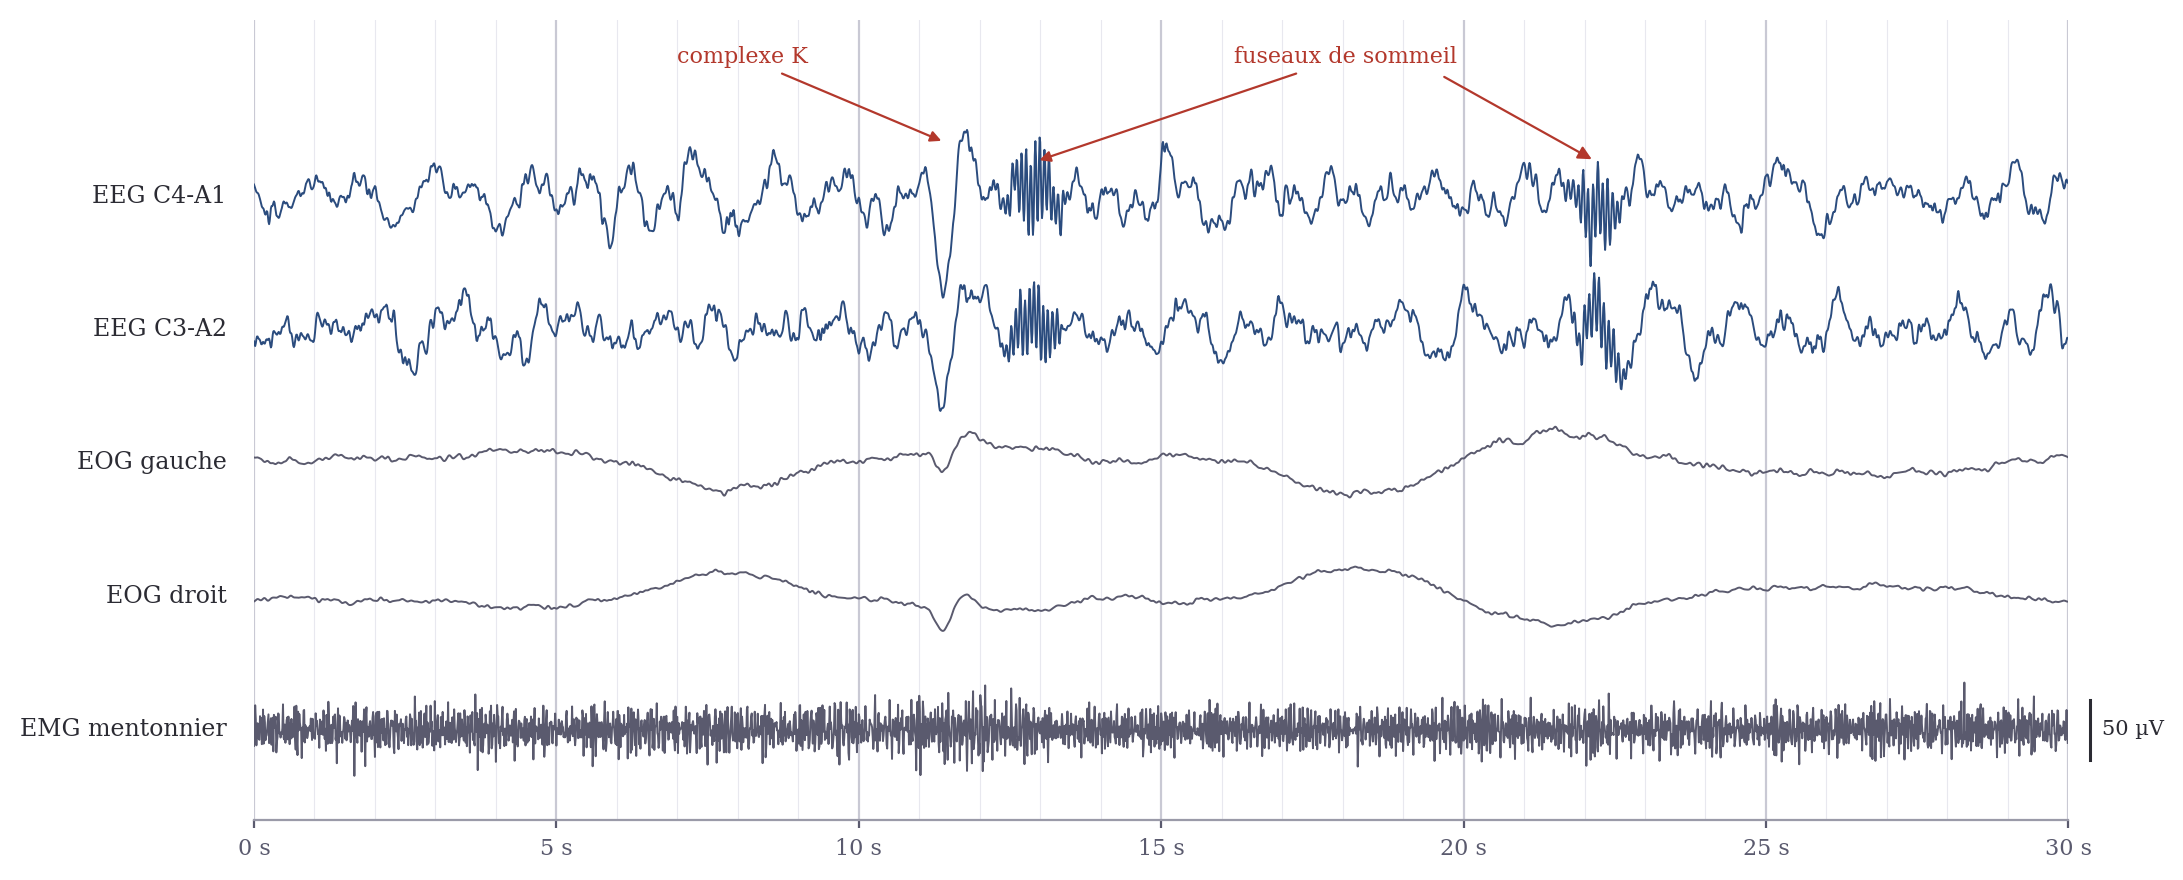
\includegraphics[width=\textwidth]{images/polysomnogramme.png}
\caption[Époque polysomnographique de 30 secondes]%
        {Tracé illustratif d'une époque de 30 secondes en stade N2. Le complexe K et les
         deux fuseaux portés par les dérivations centrales sont les grapho-éléments qui
         définissent ce stade ; l'électro-oculogramme ne montre aucun mouvement rapide
         et l'électromyogramme mentonnier garde un tonus de fond.}
\label{fig:psg-epoque}
\end{figure}

\begin{table}[H]
\centering

\small
\begin{tabular}{@{}llL{7.2cm}@{}}
\toprule
\textbf{Signal} & \textbf{Nombre} & \textbf{Apport au scorage} \\
\midrule
Électroencéphalogramme (EEG) & 2 & Rythme de fond, fuseaux, complexes K et ondes
lentes : c'est le signal qui porte la décision \\
\addlinespace[2pt]
Électro-oculogramme (EOG) & 2 & Distingue les mouvements oculaires lents de
l'endormissement des mouvements rapides du sommeil paradoxal \\
\addlinespace[2pt]
Électromyogramme (EMG) mentonnier & 1 & Le tonus musculaire sépare le sommeil
paradoxal du sommeil lent : son effondrement signe le REM \\
\bottomrule
\end{tabular}
\caption{Dérivations minimales d'un montage polysomnographique de scorage}
\label{tab:derivations}
\end{table}

Un montage complet comporte en pratique d'autres capteurs (flux nasal, sangles
thoraciques, oxymétrie de pouls, électrocardiogramme) destinés à la caractérisation
des événements respiratoires. Le scorage des stades, lui, ne requiert que les cinq
dérivations ci-dessus. Cette distinction a une conséquence pratique : elle rend
possible un système compatible avec des montages allégés, et nous évaluerons d'ailleurs une configuration
réduite à deux dérivations.

\subsection{Le syndrome d'apnées obstructives du sommeil}

Le syndrome d'apnées obstructives du sommeil (SAOS) résulte d'obstructions répétées des
voies aériennes supérieures pendant le sommeil. Chaque obstruction provoque une
désaturation en oxygène et un micro-éveil, invisible pour le patient mais destructeur
pour l'architecture du sommeil.

Sa prévalence est élevée : une analyse publiée en 2019 estime à environ
936 millions le nombre d'adultes de 30 à 69 ans présentant un SAOS léger à sévère dans
le monde, dont près de 425 millions sous une forme modérée à
sévère~\cite{benjafield2019}. Non traité, le syndrome est associé à une surmorbidité
cardiovasculaire documentée~\cite{marin2005}, et il reste largement
sous-diagnostiqué~\cite{young1997}.

La sévérité s'exprime par l'index d'apnées-hypopnées, nombre moyen d'événements
respiratoires par heure de sommeil. Le référentiel AASM~\cite{kapur2017} en définit
quatre classes, reprises au tableau~\ref{tab:iah}, qui constituent les classes cibles
du second modèle développé dans ce mémoire.

\begin{table}[H]
\centering

\small
\begin{tabular}{@{}lcL{7.4cm}@{}}
\toprule
\textbf{Classe} & \textbf{IAH (évén./h)} & \textbf{Conduite habituelle} \\
\midrule
Normal   & $< 5$          & Pas de traitement spécifique \\
Léger    & $5$ à $< 15$   & Mesures hygiéno-diététiques, surveillance \\
Modéré   & $15$ à $< 30$  & Traitement discuté selon la symptomatologie \\
Sévère   & $\geq 30$      & Traitement par pression positive continue indiqué \\
\bottomrule
\end{tabular}
\caption{Classes de sévérité du SAOS selon l'index d'apnées-hypopnées}
\label{tab:iah}
\end{table}

Au-delà des événements respiratoires qu'il provoque, le SAOS déforme l'architecture du
sommeil.
Les micro-éveils répétés fragmentent la nuit, suppriment le sommeil profond et
raccourcissent les épisodes paradoxaux. Cette empreinte est mesurable sur le seul
hypnogramme, indépendamment des capteurs respiratoires, hypothèse sur laquelle repose
le second volet du projet.

\subsection{Objectif général du projet}

\hypnoria{} est une plateforme web d'aide à l'interprétation polysomnographique
destinée aux médecins du sommeil. Elle poursuit quatre objectifs :

\begin{enumerate}[itemsep=3pt,topsep=4pt]
  \item \textbf{Automatiser le scorage des stades} à partir d'un fichier
        d'enregistrement brut au format EDF, avec une exactitude comparable à l'accord
        inter-expert.
  \item \textbf{Prédire la sévérité du SAOS} à partir de l'architecture du sommeil et
        de marqueurs cliniques, sans exiger l'annotation manuelle des événements
        respiratoires.
  \item \textbf{Expliquer chaque prédiction} en exposant les facteurs qui l'ont
        déterminée, afin que le praticien puisse la valider ou la contester.
  \item \textbf{Fournir la chaîne applicative complète} : dossier patient, archivage
        sécurisé, annotation, compte rendu exportable, collaboration et administration
        multi-établissements.
\end{enumerate}

\subsection{Problématique}

Trois constats fondent ce projet.

\subsubsection{Le coût du scorage manuel}

Une nuit d'enregistrement de huit heures produit environ un millier d'époques de
30 secondes. Chacune doit être examinée, comparée à ses voisines et classée par un
technicien qualifié. L'opération représente plusieurs heures de travail expert par
patient, auxquelles s'ajoutent l'analyse des événements respiratoires et la rédaction du
compte rendu. Dans un service saturé, le facteur limitant n'est plus le nombre de lits
d'enregistrement mais le temps d'expertise disponible pour interpréter ce qu'ils
produisent.

\subsubsection{La variabilité inter-scoreur}

Le scorage manuel est en outre imparfaitement reproductible. Le programme de fiabilité
inter-scoreurs de l'AASM mesure un accord
global de l'ordre de \SI{83}{\percent}~\cite{rosenberg2013}, avec des écarts marqués
selon le stade~\cite{danker2009}.

Deux conséquences en découlent. La première est méthodologique : les annotations de
référence ne sont pas une vérité absolue mais l'opinion d'un scoreur, et l'accord
inter-expert constitue donc un plafond de performance réaliste. La seconde est
clinique : elle légitime l'automatisation, car un modèle présente au moins la propriété
d'être parfaitement reproductible.

\subsubsection{L'opacité des modèles d'apprentissage profond}

Depuis 2017, les réseaux de neurones profonds atteignent sur les bases publiques des
performances comparables à celles d'un scoreur humain~\cite{supratak2017,perslev2021}.
Le verrou s'est donc déplacé de la précision vers l'adoption.

Un modèle d'apprentissage profond fonctionne comme une boîte noire : il produit une
classe sans énoncer ce qui l'a déterminée. Or le praticien engage sa responsabilité sur
le diagnostic qu'il signe, et ne peut ni valider ni contester une décision dont il
ignore les motifs. À ce frein pratique s'ajoute un cadre réglementaire européen qui
reconnaît un droit à l'explication pour les décisions automatisées~\cite{goodman2017}.

\medskip
\noindent
Ces trois constats convergent : la médecine du sommeil a besoin d'un système qui soit à
la fois rapide, pour absorber le volume d'examens, reproductible,
pour lever la variabilité inter-scoreur, et transparent, pour que le praticien
puisse s'en porter garant.

\section{Étude préalable}

\subsection{Étude de l'existant}

\subsubsection{Les solutions commerciales}

Le marché de l'analyse polysomnographique est dominé par des logiciels propriétaires
adossés à du matériel d'acquisition : \emph{Noxturnal} de Nox Medical, \emph{Sleepware
G3} de Philips Respironics, \emph{ProFusion PSG} de Compumedics ou encore
\emph{SleepWorks} de Natus. Une seconde génération d'acteurs, dont \emph{EnsoSleep}
d'EnsoData, propose un scorage automatique fondé sur l'apprentissage profond.

Le tableau~\ref{tab:commerciales} récapitule ces cinq suites.

\begin{table}[H]
\centering

\small
\begin{tabular}{@{}cL{2.1cm}L{2.5cm}L{2.6cm}L{2.5cm}@{}}
\toprule
& \textbf{Solution} & \textbf{Éditeur} & \textbf{Matériel associé} &
\textbf{Scorage automatique} \\
\midrule
\logoedit{noxturnal} & Noxturnal & Nox Medical, Islande & enregistreurs Nox A1 et T3 &
assisté, règles paramétrables \\
\addlinespace[3pt]
\logoedit{sleepware} & Sleepware G3 & Philips Respironics, Pays-Bas & systèmes Alice &
assisté \\
\addlinespace[3pt]
\logoedit{profusion} & ProFusion PSG & Compumedics, Australie & systèmes Grael et
Siesta & assisté \\
\addlinespace[3pt]
\logoedit{sleepworks} & SleepWorks & Natus Medical, États-Unis & plateformes Embla &
assisté \\
\addlinespace[3pt]
\logoedit{ensosleep} & EnsoSleep & EnsoData, États-Unis & indépendant du constructeur &
apprentissage profond \\
\bottomrule
\end{tabular}
\caption{Principales suites commerciales d'analyse polysomnographique}
\label{tab:commerciales}
\end{table}

En Tunisie, les laboratoires du sommeil s'appuient sur ces mêmes suites, acquises avec
le matériel d'enregistrement. Le coût de licence et l'adhérence au matériel du
constructeur en limitent la diffusion, et aucune solution nationale d'analyse
automatique n'est à notre connaissance disponible.

\subsubsection{Les travaux académiques}

La littérature scientifique a produit une succession d'architectures de plus en plus
performantes, résumées au tableau~\ref{tab:etat-art-staging}.
\emph{DeepSleepNet}~\cite{supratak2017} combine une extraction convolutive
multi-échelle et une modélisation séquentielle récurrente sur un unique canal.
\emph{TinySleepNet}~\cite{supratak2020} en propose une version allégée.
\emph{U-Sleep}~\cite{perslev2021} montre une robustesse au montage et à
la cohorte. \emph{SleepTransformer}~\cite{phan2022} introduit un mécanisme
d'auto-attention ainsi qu'une forme d'interprétabilité par les poids d'attention.
\emph{XSleepNet}~\cite{phan2021} exploite conjointement la représentation temporelle
brute et la représentation temps-fréquence.

\begin{table}[H]
\centering

\small
\begin{tabular}{@{}L{3.3cm}cL{4.4cm}L{2.2cm}c@{}}
\toprule
\textbf{Travail} & \textbf{Année} & \textbf{Approche} & \textbf{Évaluation} &
\textbf{Exactitude} \\
\midrule
Fraiwan \emph{et al.}~\cite{fraiwan2012} & 2012 & Temps-fréquence + forêt aléatoire &
jeu propriétaire & $\approx$ \SI{83}{\percent} \\
\addlinespace[2pt]
Tsinalis \emph{et al.}~\cite{tsinalis2016} & 2016 & CNN sur EEG brut & Sleep-EDF &
$\approx$ \SI{82}{\percent} \\
\addlinespace[2pt]
DeepSleepNet~\cite{supratak2017} & 2017 & CNN multi-échelle + BiLSTM & Sleep-EDF &
$\approx$ \SI{82}{\percent} \\
\addlinespace[2pt]
Chambon \emph{et al.}~\cite{chambon2018} & 2018 & CNN multivarié (EEG, EOG, EMG) &
MASS & $\approx$ \SI{83}{\percent} \\
\addlinespace[2pt]
SleepEEGNet~\cite{mousavi2019} & 2019 & CNN + séquence à séquence & Sleep-EDF &
$\approx$ \SI{84}{\percent} \\
\addlinespace[2pt]
TinySleepNet~\cite{supratak2020} & 2020 & CNN + LSTM allégés & Sleep-EDF &
$\approx$ \SI{85}{\percent} \\
\addlinespace[2pt]
AttnSleep~\cite{eldele2021} & 2021 & Multi-résolution + auto-attention & Sleep-EDF &
$\approx$ \SI{84}{\percent} \\
\addlinespace[2pt]
U-Sleep~\cite{perslev2021} & 2021 & Entièrement convolutif & 15 cohortes &
F1 macro $\approx$ 0,79 \\
\addlinespace[2pt]
SleepTransformer~\cite{phan2022} & 2022 & Transformer hiérarchique & SHHS &
$\approx$ \SI{88}{\percent} \\
\addlinespace[2pt]
XSleepNet~\cite{phan2021} & 2022 & Fusion brut + temps-fréquence & SHHS &
$\approx$ \SI{89}{\percent} \\
\bottomrule
\end{tabular}
\caption{Principaux travaux de classification automatique des stades du sommeil}
\label{tab:etat-art-staging}
\end{table}

\subsection{Critique de l'existant}

Les suites commerciales sont matures et validées cliniquement, mais présentent quatre
limites au regard de notre problématique. L'adhérence matérielle contraint les
laboratoires disposant d'un parc hétérogène. Le coût de licence, calibré pour
des structures hospitalières occidentales, reste hors de portée de nombreux centres.
L'installation locale est peu compatible avec le travail à distance et la
collaboration entre praticiens de sites différents. Enfin, lorsqu'un scorage
automatique est proposé, il l'est sans explication des facteurs qui l'ont
produit.

Les travaux académiques, de leur côté, visent la performance de classification évaluée
sur des jeux publics et s'arrêtent au modèle. Aucun ne livre la chaîne applicative qui
permettrait à un praticien d'en faire usage : gestion des patients, archivage des
examens, production d'un compte rendu, collaboration.

Le tableau~\ref{tab:existant} confronte les suites commerciales aux besoins identifiés.

\begin{table}[H]
\centering

\small
\begin{tabular}{@{}L{6.0cm}cc@{}}
\toprule
\textbf{Critère} & \textbf{Suites commerciales} & \textbf{\hypnoria{}} \\
\midrule
Scorage automatique                & partiel   & oui \\
Indépendance au matériel           & faible    & oui \\
Explicabilité des décisions        & non       & oui \\
Prédiction de la sévérité SAOS     & indirecte & oui \\
Application web multi-utilisateurs & non       & oui \\
Dossier patient et historique      & oui       & oui \\
Collaboration entre praticiens     & non       & oui \\
Traçabilité et audit               & partielle & oui \\
Coût d'acquisition                 & élevé     & nul \\
\bottomrule
\end{tabular}
\caption{Positionnement de \hypnoria{} face aux suites commerciales}
\label{tab:existant}
\end{table}

\subsection{Solution proposée}

Il ressort de cette analyse un espace non couvert, à l'intersection des deux familles :
une plateforme applicative complète, indépendante du matériel d'acquisition, qui intègre
des modèles de l'état de l'art \emph{et} les explique. C'est cet espace que le projet
occupe.

Le système s'articule autour de deux étages d'apprentissage successifs et d'une
plateforme qui les met à disposition. Le premier étage assure la classification
des stades : trois familles d'architectures (convolutive, récurrente et
attentionnelle) sont entraînées séparément puis combinées par un méta-apprenant. Deux
configurations de montage et deux granularités de sortie sont proposées, afin de couvrir
aussi bien l'enregistrement de laboratoire que le dispositif ambulatoire. Le second
étage assure la prédiction de la sévérité : il extrait de l'hypnogramme
produit une vingtaine de marqueurs d'architecture du sommeil, les complète de données
cliniques et oxymétriques, et prédit la classe de sévérité en accompagnant chaque
prédiction de sa décomposition en contributions par variable.

\section{Méthodologie de travail}

\subsection{Choix du cadre Scrum}

Le projet présentait deux sources d'incertitude difficilement compatibles avec une
planification linéaire. La première tenait aux données : l'accès aux cohortes cliniques
est soumis à une autorisation dont le délai d'instruction n'était pas connu à l'avance.
La seconde tenait aux modèles : rien ne garantissait \emph{a priori} qu'une
architecture donnée atteindrait le niveau de performance visé, ni que l'empilement
apporterait un gain.

Une démarche séquentielle aurait figé des décisions avant de disposer des éléments
permettant de les prendre. Nous avons donc retenu le cadre Scrum~\cite{schwaber2020},
dont le principe est d'avancer par incréments courts et d'ajuster la suite à ce que
chaque incrément a révélé.

\subsection{Les rôles dans la méthodologie Scrum}

Scrum définit trois rôles. Le \emph{Product Owner} porte la vision du produit, arbitre
les priorités du backlog et valide la valeur livrée. Le \emph{Scrum Master} garantit le
respect du cadre, anime les cérémonies et lève les obstacles. L'\emph{équipe de
développement} réalise l'incrément.

Le projet étant mené par une seule personne, ces rôles ont été redistribués sans être
dénaturés : la fonction de Product Owner a été portée par l'encadrement professionnel du
CNI, celle de Scrum Master par l'encadrement académique lors des points de suivi, et
celle d'équipe de développement par l'étudiant.

\subsection{Adaptation au projet}

La durée d'itération a été portée à quatre semaines plutôt que deux. Ce choix est
directement lié à la nature du travail : l'entraînement d'un modèle profond sur près de
deux cent mille exemples se compte en heures de calcul, et douze variantes devaient être
produites. Une itération de deux semaines n'aurait pas permis de livrer un incrément
évaluable pendant la phase de modélisation.

Trois artefacts ont été tenus à jour : le \emph{Product Backlog}, liste priorisée des
fonctionnalités attendues ; le \emph{Sprint Backlog}, sous-ensemble sélectionné pour
l'itération en cours ; et l'\emph{incrément}, version fonctionnelle livrée en fin de
sprint. Les cérémonies ont été condensées : une réunion de planification en début de
sprint, un point hebdomadaire avec l'encadrement en substitution de la mêlée
quotidienne, une revue de sprint sous forme de démonstration et une rétrospective
écrite.

\subsection{Organisation en releases}

Au-dessus du sprint, un second niveau de planification a été retenu : la
release, version livrable du produit qui regroupe plusieurs sprints autour d'un
objectif de valeur commun. Ce niveau répond à une réalité du projet : un sprint isolé,
comme celui consacré à l'entraînement des modèles, ne produit pas toujours à lui seul une
version exploitable, alors que deux sprints consécutifs orientés vers un même objectif le
peuvent.

Le projet a ainsi été planifié en trois releases de deux sprints chacune. Chaque
release s'ouvre par la constitution de son backlog, sous-ensemble du \emph{Product Backlog}
qu'elle s'engage à livrer, et se clôt par une revue au cours de laquelle l'incrément est
démontré dans son ensemble, suivie d'une rétrospective qui oriente la release suivante
(figure~\ref{fig:scrum}). Ce découpage structure les chapitres de réalisation du présent
mémoire : chacun est consacré à une release.

\begin{figure}[H]
\centering
\begin{tikzpicture}[
    box/.style   = {rectangle,rounded corners=2pt,draw=hypnoblue!55,fill=hypnolight,
                    align=center,font=\scriptsize,minimum height=1.15cm,text width=1.95cm},
    dark/.style  = {rectangle,rounded corners=2pt,draw=hypnored!70,fill=hypnored!8,
                    align=center,font=\scriptsize,minimum height=1.15cm,text width=1.95cm},
    fl/.style    = {-{Latex[length=2.2mm]},hypnoblue!70,line width=0.8pt},
    lab/.style   = {font=\scriptsize\itshape,text=hypnogray},
  ]

  \node[box]  (backlog) at (0,0)     {\textbf{Product\\ Backlog}\\[1pt] 60 récits};
  \node[box]  (prel)    at (2.6,0)   {\textbf{Planification\\ de release}\\[1pt] backlog
                                      de release};
  \node[box]  (psp)     at (5.35,0)  {\textbf{Planification\\ du sprint}\\[1pt] sélection
                                      et estimation};
  \node[dark] (sprint)  at (7.95,0)  {\textbf{Sprint}\\[1pt] 4 semaines};
  \node[box]  (rsp)     at (10.55,0) {\textbf{Revue et\\ rétrospective}\\[1pt] du sprint};
  \node[box]  (rrel)    at (13.3,0)  {\textbf{Revue de\\ release}\\[1pt] incrément
                                      livrable};

  % Boucle des sprints d'une release
  \draw[hypnored!55,dashed,rounded corners=4pt,line width=0.6pt]
       (4.1,-0.8) rectangle (11.8,1.55);
  \node[lab,text=hypnored!85,anchor=south east] at (11.8,1.58)
       {deux sprints par release};

  \draw[fl] (backlog) -- (prel);
  \draw[fl] (prel)    -- (psp);
  \draw[fl] (psp)     -- (sprint);
  \draw[fl] (sprint)  -- (rsp);
  \draw[fl] (rsp)     -- (rrel);

  \draw[fl] (rsp.north) -- ++(0,0.55) -- node[lab,below,pos=0.5] {sprint suivant}
        ++(-5.2,0) -- (psp.north);

  % Boucle des releases
  \draw[fl] (rrel.south) -- ++(0,-0.75) -- node[lab,below,pos=0.5]
        {release suivante : réalimentation du backlog} ++(-13.3,0) -- (backlog.south);

\end{tikzpicture}
\vspace{0.4cm}
\caption[Cycle Scrum adapté au projet]%
        {Cycle Scrum adapté à un projet individuel de six mois, organisé en releases de
         deux sprints.}
\label{fig:scrum}
\end{figure}

\sectionsansnum{Conclusion}

Ce chapitre a posé le cadre du projet. Nous avons présenté le Centre National de
l'Informatique et montré comment trois de ses contraintes structurantes ont orienté les
choix techniques. Nous avons ensuite introduit les notions médicales nécessaires : les
cinq stades du référentiel AASM, l'hypnogramme, le montage polysomnographique et les
classes de sévérité du SAOS.

De ce contexte se dégage une problématique à trois volets : le coût du scorage manuel,
sa variabilité entre experts et l'opacité des modèles qui prétendent l'automatiser.
L'étude de l'existant a montré que les suites commerciales et les travaux académiques
traitent chacun une partie du problème sans le couvrir entièrement, laissant ouvert
l'espace qu'occupe \hypnoria{}.

Le chapitre suivant traduit ces intentions en une spécification vérifiable : acteurs,
besoins fonctionnels et non fonctionnels, backlog du produit, modèle de données,
architecture globale et planification des releases.
    % Presentation generale
\chapter{Analyse et spécification des besoins}
\label{chap:analyse}

\sectionsansnum{Introduction}

Le chapitre précédent a établi ce qu'il fallait construire et pourquoi. Celui-ci
formalise la commande. Nous identifions d'abord les acteurs du système et leurs
responsabilités, puis nous exprimons les besoins fonctionnels et non fonctionnels. Ces
besoins sont ensuite traduits en un \emph{Product Backlog} de soixante récits
utilisateur, priorisés et estimés. Nous présentons enfin le modèle de données,
l'environnement de travail, l'architecture globale et la planification du backlog en trois
releases de deux sprints chacune, qui structure les trois chapitres suivants.

\section{Identification des acteurs}

Un acteur désigne toute entité qui interagit avec le système sans en faire partie. On
distingue les acteurs \emph{principaux}, qui déclenchent les cas d'utilisation pour en
retirer une valeur, des acteurs \emph{secondaires}, sollicités par le système pour
mener une opération à bien. Le tableau~\ref{tab:acteurs} recense les quatre acteurs de
\hypnoria{}.

\begin{table}[H]
\centering

\small
\begin{tabular}{@{}L{3.0cm}cL{8.2cm}@{}}
\toprule
\textbf{Acteur} & \textbf{Type} & \textbf{Responsabilités} \\
\midrule
Médecin du sommeil & principal &
Constituer et suivre son registre de patients, lancer l'analyse d'un enregistrement,
interpréter l'hypnogramme et la prédiction de sévérité, annoter, produire le compte
rendu, solliciter un confrère \\
\addlinespace[3pt]
Administrateur & principal &
Créer et administrer les comptes médecins, gérer les échéances de licence, rattacher
les praticiens à un établissement, superviser l'activité et consulter le journal
d'audit \\
\addlinespace[3pt]
Moteur d'inférence & secondaire &
Charger les modèles, prétraiter le signal, produire la séquence de stades, calculer
les métriques et les attributions d'explication \\
\addlinespace[3pt]
Service de stockage & secondaire &
Recevoir les fichiers volumineux, les conserver de façon durable et délivrer des liens
d'accès temporaires \\
\bottomrule
\end{tabular}
\caption{Acteurs du système et leurs responsabilités}
\label{tab:acteurs}
\end{table}

Deux remarques sur ce découpage. Le moteur d'inférence est modélisé comme un
acteur distinct bien qu'il réside dans le même processus que l'interface applicative :
ce choix matérialise le fait qu'il pourrait être déporté sur une machine dédiée sans
modifier les cas d'utilisation. Le service de stockage, lui, est réellement
externe.

\section{Étude des besoins}

\subsection{Les besoins fonctionnels}

Les besoins fonctionnels ont été organisés en neuf \emph{épics}, regroupements
thématiques de fonctionnalités partageant un même objectif métier. Cette structure,
présentée au tableau~\ref{tab:epics}, sert de colonne vertébrale au backlog. Les épics
y sont rangés dans l'ordre où ils ont été traités : les deux étages d'apprentissage
d'abord, puis la restitution au praticien, et enfin la plateforme, sa gouvernance et son
déploiement.

\begin{table}[H]
\centering

\small
\begin{tabular}{@{}clL{7.4cm}cc@{}}
\toprule
\textbf{Épic} & \textbf{Intitulé} & \textbf{Portée} & \textbf{Récits} &
\textbf{Points} \\
\midrule
E1 & Classification & Lecture EDF, prétraitement, modèles de base, métriques AASM
& 12 & 95 \\
\addlinespace[2pt]
E2 & Sévérité du SAOS & Empilement, extraction de marqueurs, prédiction, explications
& 8 & 65 \\
\addlinespace[2pt]
E3 & Visualisation & Hypnogramme, oxymétrie, annotation, normes de référence & 5 & 28 \\
\addlinespace[2pt]
E4 & Authentification & Connexion, jetons, hachage, contrôle des rôles, application des
licences & 5 & 18 \\
\addlinespace[2pt]
E5 & Dossier patient & Registre des patients, examens, historique, tableau de bord
& 6 & 24 \\
\addlinespace[2pt]
E6 & Archivage et export & Stockage cloud, liens signés, compte rendu, exports
& 6 & 36 \\
\addlinespace[2pt]
E7 & Administration & Comptes médecins, cycle de vie, établissements, audit,
statistiques & 10 & 45 \\
\addlinespace[2pt]
E8 & Collaboration & Discussions rattachées à un examen, boîte de réception & 3 & 18 \\
\addlinespace[2pt]
E9 & Industrialisation & Conteneurisation, intégration continue, déploiement,
multilinguisme & 5 & 29 \\
\midrule
\multicolumn{3}{@{}r}{\textbf{Total}} & \textbf{60} & \textbf{358} \\
\bottomrule
\end{tabular}
\caption{Regroupement des besoins fonctionnels en épics}
\label{tab:epics}
\end{table}

\subsection{Les besoins non fonctionnels}

Les exigences non fonctionnelles conditionnent l'acceptabilité du système autant que
ses fonctions. Elles sont d'autant plus contraignantes ici que le domaine, la donnée
de santé, impose des obligations propres. Le tableau~\ref{tab:bnf} les énonce avec,
pour chacune, le moyen de vérification retenu : un besoin non fonctionnel qu'on ne sait
pas vérifier n'est qu'une intention.

\begin{table}[H]
\centering

\small
\begin{tabular}{@{}L{2.7cm}L{5.6cm}L{5.6cm}@{}}
\toprule
\textbf{Critère} & \textbf{Exigence} & \textbf{Vérification} \\
\midrule
Sécurité &
Aucun accès sans jeton valide ; mots de passe jamais stockés en clair ; cloisonnement
strict entre rôles &
Revue des dépendances de sécurité sur chaque route ; tentative d'accès croisé entre
comptes \\
\addlinespace[3pt]
Confidentialité &
Aucun fichier patient accessible par une URL publique ou devinable &
Vérification que tout lien délivré est signé et expire \\
\addlinespace[3pt]
Traçabilité &
Toute action sensible horodatée avec son auteur, journal exportable &
Inspection du journal après un scénario complet \\
\addlinespace[3pt]
Performance &
Analyse d'une nuit complète en quelques minutes ; interface non bloquée pendant les
transferts &
Chronométrage sur enregistrements réels ; transfert en arrière-plan observable \\
\addlinespace[3pt]
Interopérabilité &
Accepter les fichiers EDF quel que soit le constructeur ; importer et exporter en
formats ouverts &
Résolution des canaux sur des enregistrements de provenances différentes \\
\addlinespace[3pt]
Ergonomie &
Parcours d'analyse guidé, sans formation préalable ; retour visuel sur les traitements
longs &
Passage d'un utilisateur non initié sur le parcours complet \\
\addlinespace[3pt]
Multilinguisme &
Interface intégralement disponible en français et en anglais &
Revue de l'absence de chaînes non traduites \\
\addlinespace[3pt]
Portabilité &
Déploiement complet sur une machine vierge sans configuration manuelle &
Démarrage de la pile sur un poste neuf en une commande \\
\addlinespace[3pt]
Maintenabilité &
Séparation nette des responsabilités ; ajout d'un modèle sans toucher au reste &
Ajout d'une variante de modèle à titre d'essai \\
\bottomrule
\end{tabular}
\caption{Besoins non fonctionnels et moyens de vérification}
\label{tab:bnf}
\end{table}

\section{Diagramme de cas d'utilisation global}

La figure~\ref{fig:uc-global} présente la vue d'ensemble des interactions entre les
acteurs et le système.

\begin{figure}[H]
\centering
\begin{tikzpicture}[
    x=1cm,y=1cm,
    uc/.style      = {ellipse, draw=hypnoblue!60, fill=hypnolight,
                      align=center, font=\scriptsize, text width=2.45cm,
                      inner sep=1.5pt, minimum height=0.92cm},
    lien/.style    = {hypnogray!75, line width=0.5pt},
    nomact/.style  = {font=\scriptsize\bfseries, align=center, text width=2.2cm},
  ]

  % ── Pictogramme d'acteur ────────────────────────────────────────────────
  \tikzset{acteur/.pic={
      \draw[hypnoblue,line width=0.8pt] (0,0) circle (0.17);
      \draw[hypnoblue,line width=0.8pt] (0,-0.17) -- (0,-0.66);
      \draw[hypnoblue,line width=0.8pt] (-0.28,-0.34) -- (0.28,-0.34);
      \draw[hypnoblue,line width=0.8pt] (0,-0.66) -- (-0.24,-1.04);
      \draw[hypnoblue,line width=0.8pt] (0,-0.66) -- (0.24,-1.04);}}

  % ── Frontière du système ────────────────────────────────────────────────
  \draw[hypnoblue!55,line width=0.9pt,rounded corners=3pt]
       (3.45,-6.40) rectangle (11.05,2.55);
  \node[font=\small\bfseries,text=hypnoblue,anchor=north] at (7.25,2.42)
       {Système \hypnoria{}};

  % ── Cas d'utilisation ───────────────────────────────────────────────────
  \node[uc] (auth)  at (7.25, 1.20) {S'authentifier};

  \node[uc] (pat)   at (5.35,-0.40) {Gérer ses patients};
  \node[uc] (ana)   at (5.35,-1.70) {Analyser un\\enregistrement};
  \node[uc] (osa)   at (5.35,-3.00) {Prédire la\\sévérité du SAOS};
  \node[uc] (annot) at (5.35,-4.30) {Annoter et\\exporter};
  \node[uc] (colab) at (5.35,-5.60) {Solliciter un\\confrère};

  \node[uc] (comp)  at (9.15,-0.40) {Gérer les comptes\\et licences};
  \node[uc] (etab)  at (9.15,-1.70) {Gérer les\\établissements};
  \node[uc] (audit) at (9.15,-3.00) {Consulter le\\journal d'audit};
  \node[uc] (stats) at (9.15,-4.30) {Suivre l'activité\\de la plateforme};

  % ── Acteurs principaux : libellé au-dessus, liaisons vers la droite ─────
  \pic at (1.15,0.00) {acteur};
  \node[nomact,anchor=south] at (1.15,0.42) {Médecin\\du sommeil};

  \pic at (13.35,0.00) {acteur};
  \node[nomact,anchor=south] at (13.35,0.42) {Administrateur};

  \foreach \c in {auth,pat,ana,osa,annot,colab}
    \draw[lien] (1.50,-0.20) -- (\c.west);

  \foreach \c in {auth,comp,etab,audit,stats}
    \draw[lien] (13.00,-0.20) -- (\c.east);

  % ── Acteurs secondaires : libellé en dessous ────────────────────────────
  \pic at (7.25,-7.55) {acteur};
  \node[nomact,anchor=north] at (7.25,-8.72) {Moteur\\d'inférence};

  \pic at (10.35,-7.55) {acteur};
  \node[nomact,anchor=north] at (10.35,-8.72) {Service de\\stockage};

  \draw[lien] (7.25,-7.28) -- (ana.east);
  \draw[lien] (7.25,-7.28) -- (osa.east);
  \draw[lien] (10.35,-7.28) -- (annot.east);

\end{tikzpicture}
\vspace{0.2cm}
\caption[Diagramme de cas d'utilisation global]%
        {Vue d'ensemble des cas d'utilisation de \hypnoria{}.}
\label{fig:uc-global}
\end{figure}

Le cas « Analyser un enregistrement » constitue le c\oe ur fonctionnel du système. La
figure~\ref{fig:uc-analyse} le décompose et fait apparaître les relations d'inclusion
(sous-cas systématiquement exécutés) et d'extension (comportements optionnels).

\begin{figure}[H]
\centering
\begin{tikzpicture}[
    x=1cm,y=1cm,
    uc/.style      = {ellipse, draw=hypnoblue!60, fill=hypnolight,
                      align=center, font=\scriptsize, text width=2.5cm,
                      inner sep=1.5pt, minimum height=0.92cm},
    ucp/.style     = {ellipse, draw=hypnored!75, fill=hypnored!8,
                      align=center, font=\scriptsize\bfseries, text width=2.5cm,
                      inner sep=1.5pt, minimum height=0.92cm},
    lien/.style    = {hypnogray!75, line width=0.5pt},
    incl/.style    = {-{Latex[length=2mm]}, hypnoblue!75, line width=0.5pt, dashed},
    ext/.style     = {-{Latex[length=2mm]}, hypnored!70, line width=0.5pt, dashed},
    et/.style      = {font=\tiny\itshape, fill=white, inner sep=1.2pt},
    nomact/.style  = {font=\scriptsize\bfseries, align=center, text width=1.8cm},
  ]

  \tikzset{acteur/.pic={
      \draw[hypnoblue,line width=0.8pt] (0,0) circle (0.17);
      \draw[hypnoblue,line width=0.8pt] (0,-0.17) -- (0,-0.66);
      \draw[hypnoblue,line width=0.8pt] (-0.28,-0.34) -- (0.28,-0.34);
      \draw[hypnoblue,line width=0.8pt] (0,-0.66) -- (-0.24,-1.04);
      \draw[hypnoblue,line width=0.8pt] (0,-0.66) -- (0.24,-1.04);}}

  % ── Frontière ───────────────────────────────────────────────────────────
  \draw[hypnoblue!55,line width=0.9pt,rounded corners=3pt]
       (2.75,-4.55) rectangle (12.60,3.15);
  \node[font=\small\bfseries,text=hypnoblue,anchor=north] at (7.65,3.02)
       {Module d'analyse};

  % ── Cas central et cas déclenchés par le médecin ────────────────────────
  \node[ucp] (ana) at (4.75, 0.75) {Analyser un\\enregistrement};
  \node[uc]  (exp) at (4.75,-2.20) {Exporter les\\marqueurs};
  \node[uc]  (pdf) at (4.75,-3.65) {Produire le\\compte rendu};

  % ── Sous-cas inclus ─────────────────────────────────────────────────────
  \node[uc] (chn) at (10.30, 2.10) {Choisir le montage\\et la granularité};
  \node[uc] (pre) at (10.30, 0.85) {Prétraiter\\le signal};
  \node[uc] (cls) at (10.30,-0.40) {Classer les époques};
  \node[uc] (met) at (10.30,-1.75) {Calculer les\\métriques AASM};

  % ── Cas étendu ──────────────────────────────────────────────────────────
  \node[uc] (osa) at (10.30,-3.65) {Prédire la\\sévérité};

  % ── Acteur ──────────────────────────────────────────────────────────────
  \pic at (1.05,0.55) {acteur};
  \node[nomact,anchor=south] at (1.05,0.97) {Médecin};

  \draw[lien] (1.40,0.35) -- (ana.west);
  \draw[lien] (1.40,0.35) -- (exp.west);
  \draw[lien] (1.40,0.35) -- (pdf.west);

  % ── Relations d'inclusion (libellés étagés le long du faisceau) ──────────
  \draw[incl] (ana) -- node[et,text=hypnoblue!85,pos=0.30] {$\ll$include$\gg$} (chn);
  \draw[incl] (ana) -- node[et,text=hypnoblue!85,pos=0.44] {$\ll$include$\gg$} (pre);
  \draw[incl] (ana) -- node[et,text=hypnoblue!85,pos=0.58] {$\ll$include$\gg$} (cls);
  \draw[incl] (ana) -- node[et,text=hypnoblue!85,pos=0.72] {$\ll$include$\gg$} (met);

  % ── Relations d'extension ───────────────────────────────────────────────
  \draw[ext] (osa) -- node[et,text=hypnored!85,pos=0.5] {$\ll$extend$\gg$} (met);
  \draw[ext] (pdf) -- node[et,text=hypnored!85,pos=0.5] {$\ll$extend$\gg$} (exp);

\end{tikzpicture}
\vspace{0.2cm}
\caption[Raffinement du cas « Analyser un enregistrement »]%
        {Décomposition du cas d'utilisation central en sous-cas inclus et étendus.}
\label{fig:uc-analyse}
\end{figure}

Les tableaux~\ref{tab:desc-analyse} et~\ref{tab:desc-osa} décrivent textuellement les
deux cas les plus critiques. Un diagramme montre en effet la structure des interactions,
mais pas leur déroulement.

\begin{table}[H]
\centering

\small
\begin{tabular}{@{}L{3.0cm}L{11.4cm}@{}}
\toprule
\textbf{Identifiant} & UC-03 \\
\textbf{Acteur principal} & Médecin du sommeil \\
\textbf{Acteurs secondaires} & Moteur d'inférence, service de stockage \\
\textbf{Préconditions} & Le médecin est authentifié ; sa licence est valide ; il
dispose d'un fichier d'enregistrement au format EDF \\
\textbf{Postconditions} & Un examen est créé dans le dossier du patient, la séquence
de stades et les métriques sont enregistrées, le fichier brut est archivé \\
\midrule
\textbf{Scénario nominal} &
\begin{minipage}[t]{11.2cm}
\begin{enumerate}[leftmargin=1.1em,itemsep=1pt,topsep=2pt]
  \item Le médecin sélectionne le patient concerné.
  \item Il choisit le montage disponible, à deux ou cinq dérivations.
  \item Il choisit la granularité de classification, à trois ou cinq stades.
  \item Il dépose le fichier d'enregistrement.
  \item Le système décode le fichier, résout les dérivations et prétraite le signal.
  \item Le moteur d'inférence classe chaque époque et le système calcule les métriques.
  \item Le système affiche l'hypnogramme, les métriques et les alertes cliniques.
  \item Le système crée l'examen et lance l'archivage du fichier en arrière-plan.
\end{enumerate}
\end{minipage} \\
\midrule
\textbf{Scénarios alternatifs} &
\begin{minipage}[t]{11.2cm}
\begin{itemize}[leftmargin=1.1em,itemsep=1pt,topsep=2pt]
  \item \textbf{4a} --- Le fichier n'est pas au format attendu : le système refuse le
        dépôt et le signale.
  \item \textbf{5a} --- Une dérivation est absente : le système applique son repli
        documenté et poursuit.
  \item \textbf{5b} --- L'enregistrement est plus court qu'une époque : le traitement
        s'interrompt avec un message explicite.
  \item \textbf{8a} --- L'archivage échoue : les résultats restent consultables et le
        transfert est signalé en erreur.
\end{itemize}
\end{minipage} \\
\bottomrule
\end{tabular}
\caption{Description textuelle du cas « Analyser un enregistrement »}
\label{tab:desc-analyse}
\end{table}

\begin{table}[H]
\centering

\small
\begin{tabular}{@{}L{3.0cm}L{11.4cm}@{}}
\toprule
\textbf{Identifiant} & UC-04 \\
\textbf{Acteur principal} & Médecin du sommeil \\
\textbf{Acteur secondaire} & Moteur d'inférence \\
\textbf{Préconditions} & Une séquence de stades est disponible, issue d'une analyse ou
d'une saisie manuelle \\
\textbf{Postconditions} & Une classe de sévérité, ses probabilités et la décomposition
des facteurs sont associées à l'examen \\
\midrule
\textbf{Scénario nominal} &
\begin{minipage}[t]{11.2cm}
\begin{enumerate}[leftmargin=1.1em,itemsep=1pt,topsep=2pt]
  \item Le système extrait les marqueurs d'architecture depuis l'hypnogramme.
  \item Le médecin complète les données démographiques et oxymétriques.
  \item Il déclenche l'évaluation du risque.
  \item Le système construit le vecteur de variables et comble les valeurs absentes.
  \item Le moteur produit la classe de sévérité et ses probabilités.
  \item Le système calcule les contributions de chaque variable.
  \item Le système affiche la sévérité, les facteurs aggravants et protecteurs, et
        l'interprétation clinique.
\end{enumerate}
\end{minipage} \\
\midrule
\textbf{Scénarios alternatifs} &
\begin{minipage}[t]{11.2cm}
\begin{itemize}[leftmargin=1.1em,itemsep=1pt,topsep=2pt]
  \item \textbf{2a} --- Le médecin importe un rapport externe : le système en extrait
        les valeurs et préremplit le formulaire.
  \item \textbf{4a} --- Des variables cliniques manquent : le système applique la
        valeur médiane de la population d'apprentissage et le signale.
  \item \textbf{5a} --- Les modèles ne sont pas chargés : l'opération est refusée avec
        un message explicite.
\end{itemize}
\end{minipage} \\
\bottomrule
\end{tabular}
\caption{Description textuelle du cas « Prédire la sévérité du SAOS »}
\label{tab:desc-osa}
\end{table}

\section{Backlog du produit}

Le \emph{Product Backlog} est la liste ordonnée de tout ce que le produit doit offrir.
Chaque élément prend la forme d'un récit utilisateur suivant la formulation canonique :
\emph{en tant que} \dots, \emph{je veux} \dots, \emph{afin de} \dots. Cette
formulation force à énoncer le bénéficiaire et la finalité, et non seulement la
fonction.

Deux attributs complètent chaque récit. La priorité suit la méthode MoSCoW :
\emph{Must have} pour ce sans quoi le produit n'a pas de sens, \emph{Should have} pour
ce qui lui donne sa valeur, \emph{Could have} pour ce qui l'améliore sans le
conditionner. L'estimation s'exprime en points de complexité sur la suite de
Fibonacci, échelle relative qui compare les récits entre eux plutôt que de prétendre
prédire une durée.

L'ordre de la liste suit celui de la réalisation. Les récits d'apprentissage
automatique viennent en tête : la classification des stades, puis la prédiction de la
sévérité, parce que c'est d'eux que dépend la valeur de tout le reste et que leur
résultat était le plus incertain. Le développement de la plateforme, sa gouvernance et
son déploiement ferment la liste.

\begin{longtable}{@{}p{1.25cm}L{9.1cm}cp{0.75cm}p{0.9cm}@{}}
\caption{Product Backlog --- 60 récits utilisateur, 358 points}
\label{tab:backlog}\\
\toprule
\textbf{ID} & \textbf{Récit utilisateur} & \textbf{Prio.} & \textbf{Pts} &
\textbf{Spr.} \\
\midrule
\endfirsthead

\multicolumn{5}{@{}l}{\small\itshape Tableau~\ref{tab:backlog} --- suite}\\
\toprule
\textbf{ID} & \textbf{Récit utilisateur} & \textbf{Prio.} & \textbf{Pts} &
\textbf{Spr.} \\
\midrule
\endhead

\midrule
\multicolumn{5}{@{}r}{\small\itshape suite page suivante}\\
\endfoot

\bottomrule
\endlastfoot

\multicolumn{5}{@{}l}{\cellcolor{hypnolight}\textbf{E1 --- Classification automatique des stades}}\\
\midrule
\small
US-01 & Lire un fichier EDF et en extraire les dérivations physiologiques & M & 8 & S1 \\
US-02 & Résoudre les canaux malgré l'hétérogénéité des conventions de nommage
& M & 5 & S1 \\
US-03 & Rééchantillonner, segmenter en époques de 30 s et normaliser & M & 8 & S1 \\
US-04 & Valider la chaîne sur un jeu public en attendant l'accès aux cohortes
& M & 8 & S1 \\
US-05 & Prétraiter les enregistrements de la cohorte clinique à l'échelle & M & 8 & S2 \\
US-06 & Classer chaque époque avec un réseau convolutif multi-échelle & M & 13 & S2 \\
US-07 & Classer chaque époque avec un réseau récurrent à pooling attentionnel
& M & 13 & S2 \\
US-08 & Classer chaque époque avec un Transformer par patchs & M & 13 & S2 \\
US-09 & Choisir la configuration d'analyse selon le montage disponible & S & 5 & S4 \\
US-10 & Inspecter les canaux d'un fichier avant de lancer l'analyse & S & 3 & S4 \\
US-11 & Calculer les métriques AASM de l'enregistrement & M & 8 & S4 \\
US-12 & Conserver les modèles en mémoire entre deux requêtes & S & 3 & S4 \\

\epictitre{E2 --- Ensemble et prédiction de la sévérité}
US-13 & Combiner les trois modèles par un méta-apprenant & M & 13 & S3 \\
US-14 & Extraire les marqueurs d'architecture du sommeil depuis l'hypnogramme
& M & 8 & S3 \\
US-15 & Prédire la sévérité du SAOS en quatre classes & M & 13 & S3 \\
US-16 & Exposer les facteurs aggravants et protecteurs de la prédiction & M & 8 & S3 \\
US-17 & Saisir les données oxymétriques et les index d'éveil & M & 5 & S4 \\
US-18 & Lancer une prédiction sans fichier, à partir d'une saisie manuelle & S & 8 & S4 \\
US-19 & Importer un rapport externe pour préremplir le formulaire clinique
& S & 5 & S4 \\
US-20 & Lire une interprétation clinique automatique des anomalies détectées
& S & 5 & S4 \\

\epictitre{E3 --- Visualisation, annotation et normes}
US-21 & Visualiser l'hypnogramme de façon interactive & M & 8 & S4 \\
US-22 & Voir la saturation et la densité d'événements sur le même axe temporel
& S & 5 & S4 \\
US-23 & Suivre la progression de l'analyse en cours & C & 5 & S4 \\
US-24 & Annoter une époque précise pour consigner une observation & S & 5 & S6 \\
US-25 & Situer chaque métrique par rapport aux normes de référence & S & 5 & S6 \\

\epictitre{E4 --- Authentification et contrôle d'accès}
US-26 & Me connecter avec mon adresse et mon mot de passe pour accéder à la plateforme
& M & 5 & S4 \\
US-27 & Consulter mon profil pour vérifier mon rôle et mon rattachement & M & 2 & S4 \\
US-28 & Stocker les mots de passe hachés pour qu'aucun ne soit lisible en base
& M & 3 & S4 \\
US-29 & Vérifier le rôle sur chaque route pour cloisonner médecins et administrateurs
& M & 5 & S4 \\
US-30 & Refuser la connexion d'un compte suspendu ou dont la licence a expiré
& M & 3 & S5 \\

\epictitre{E5 --- Dossier patient et examens}
US-31 & Enregistrer un patient avec son âge, son IMC et son sexe & M & 3 & S5 \\
US-32 & Lister mes patients avec leur historique d'examens & M & 5 & S5 \\
US-33 & Consulter la fiche détaillée d'un patient et tous ses examens & M & 3 & S5 \\
US-34 & Créer un examen rattaché à un patient pour y associer les résultats
& M & 5 & S5 \\
US-35 & Mettre à jour la sévérité et les résultats d'un examen & M & 3 & S5 \\
US-36 & Voir la répartition des risques d'apnée de ma patientèle & S & 5 & S6 \\

\epictitre{E6 --- Archivage et exports}
US-37 & Archiver le fichier brut sans bloquer l'interface & M & 8 & S5 \\
US-38 & Archiver l'hypnogramme et le compte rendu clinique & S & 5 & S5 \\
US-39 & Délivrer des liens d'accès à durée limitée & M & 5 & S5 \\
US-40 & Exporter les marqueurs calculés pour un autre outil & S & 5 & S4 \\
US-41 & Composer le compte rendu en choisissant les sections à inclure & M & 8 & S6 \\
US-42 & Synchroniser l'hypnogramme annoté vers le dossier & S & 5 & S6 \\

\epictitre{E7 --- Administration de la plateforme}
US-43 & Créer un compte médecin pour ouvrir l'accès à un nouveau praticien & M & 5 & S5 \\
US-44 & Lister les médecins avec leur statut et leur échéance de licence & M & 3 & S5 \\
US-45 & Suspendre ou réactiver un compte et fixer sa date d'expiration & M & 5 & S5 \\
US-46 & Réinitialiser le mot de passe d'un médecin pour débloquer un accès perdu
& S & 3 & S5 \\
US-47 & Créer des établissements et y rattacher des médecins & S & 5 & S5 \\
US-48 & Journaliser chaque action sensible avec son auteur et son horodatage
& M & 5 & S5 \\
US-49 & Consulter le journal d'audit pour enquêter sur un incident & M & 5 & S5 \\
US-50 & Exporter le journal d'audit pour un contrôle de conformité & S & 3 & S5 \\
US-51 & Consulter les statistiques globales pour suivre l'adoption & S & 3 & S5 \\
US-52 & Visualiser la chaîne de traitement des modèles & C & 8 & S6 \\

\epictitre{E8 --- Collaboration entre praticiens}
US-53 & Ouvrir une discussion sur un examen avec un confrère & S & 8 & S6 \\
US-54 & Échanger des messages dans un fil rattaché à l'examen & S & 5 & S6 \\
US-55 & Consulter une boîte de réception centralisée & S & 5 & S6 \\

\epictitre{E9 --- Industrialisation et déploiement}
US-56 & Conteneuriser les trois services pour un déploiement reproductible
& M & 8 & S6 \\
US-57 & Orchestrer la pile en une seule commande & M & 5 & S6 \\
US-58 & Automatiser tests et construction d'images à chaque livraison & S & 8 & S6 \\
US-59 & Basculer l'interface entre français et anglais & S & 5 & S6 \\
US-60 & Basculer en thème sombre pour la lecture nocturne & C & 3 & S6 \\
\end{longtable}

\noindent
La formulation complète a été abrégée dans le tableau pour tenir sur une ligne ; le
bénéficiaire se déduit de l'épic.

\section{Diagramme de classes}

Le modèle métier s'organise autour de huit entités (figure~\ref{fig:classes}).
L'entité centrale est l'\emph{examen}, qui matérialise une nuit d'enregistrement : elle
porte les références vers les fichiers archivés, la classe de sévérité prédite et le
document de résultats. Autour d'elle gravitent le patient qui l'a subie, les annotations
que le praticien y a portées et les discussions qu'elle a suscitées.

\begin{figure}[H]
\centering
\begin{tikzpicture}[
    x=1cm,y=1cm,
    cls/.style  = {rectangle,draw=hypnoblue!65,fill=white,align=left,anchor=north,
                   font=\tiny,inner sep=0pt,text width=4.35cm},
    ent/.style  = {rectangle,draw=hypnored!70,fill=hypnored!6,align=left,anchor=north,
                   font=\tiny,inner sep=0pt,text width=4.35cm},
    rel/.style  = {hypnogray!85,line width=0.6pt},
    card/.style = {font=\tiny,text=hypnogray,inner sep=1.6pt,fill=white},
    note/.style = {font=\tiny\itshape,text=hypnogray,align=center,text width=4.2cm},
  ]

  \newcommand{\classe}[3]{%
    \begin{tabular}{@{\hspace{3pt}}>{\raggedright\arraybackslash
                             \hyphenpenalty=10000\exhyphenpenalty=10000}p{4.15cm}@{}}
      \rowcolor{hypnolight}\textbf{#1}\\[1pt]
      \hline
      \rule{0pt}{7pt}#2\\[1pt]
      \hline
      \rule{0pt}{7pt}#3\\[1pt]
    \end{tabular}}

  % ── Rangée 1 ────────────────────────────────────────────────────────────
  \node[cls] (hop) at (2.45, 6.30) {\classe{Hospital}{%
       $-$~id : int\newline
       $-$~name : str\newline
       $-$~b2\_bucket : str\newline
       $-$~billing\_tier : str\newline
       $-$~created\_at : datetime}{%
       + create\_hospital(name : str) : Hospital\newline
       + get\_hospitals() : list[Hospital]}};

  \node[cls] (usr) at (7.95, 6.30) {\classe{User}{%
       $-$~id : int\newline
       $-$~email : str\newline
       $-$~hashed\_password : str\newline
       $-$~role : str\newline
       $-$~first\_name : str\newline
       $-$~last\_name : str\newline
       $-$~status : str\newline
       $-$~license\_expiry : datetime\newline
       $-$~last\_login : datetime\newline
       $-$~hospital\_id : int}{%
       + verify\_password(plain : str) : bool\newline
       + create\_access\_token(ttl : timedelta) : str\newline
       + update\_lifecycle(status : str, expiry : datetime) : User\newline
       + reset\_password(new : str) : bool}};

  \node[cls] (pat) at (13.45, 6.30) {\classe{Patient}{%
       $-$~id : int\newline
       $-$~first\_name : str\newline
       $-$~last\_name : str\newline
       $-$~age : int\newline
       $-$~imc : float\newline
       $-$~gender : str\newline
       $-$~doctor\_id : int}{%
       + create\_patient() : Patient\newline
       + get\_patients() : list[Patient]\newline
       + get\_doctor\_stats() : dict}};

  % ── Rangée 2 ────────────────────────────────────────────────────────────
  \node[cls] (log)  at (2.45, 0.55) {\classe{AuditLog}{%
       $-$~id : int\newline
       $-$~timestamp : datetime\newline
       $-$~user\_email : str\newline
       $-$~user\_role : str\newline
       $-$~action : str\newline
       $-$~ip\_address : str}{%
       + log\_audit(action : str) : None\newline
       + get\_audit\_logs(limit : int) : list[AuditLog]\newline
       + export\_csv() : StreamingResponse}};

  \node[cls] (conv) at (7.95, 0.55) {\classe{FileConversation}{%
       $-$~id : int\newline
       $-$~psg\_id : int\newline
       $-$~file\_type : str\newline
       $-$~doctor\_one\_id : int\newline
       $-$~doctor\_two\_id : int\newline
       $-$~created\_at : datetime}{%
       + get\_or\_create() : FileConversation\newline
       + get\_my\_conversations() : list[FileConversation]\newline
       + get\_messages() : list[FileMessage]}};

  \node[ent] (psg)  at (13.45, 0.55) {\classe{PSG}{%
       $-$~id : int\newline
       $-$~patient\_id : int\newline
       $-$~date : datetime\newline
       $-$~severity : str\newline
       $-$~report\_data : str\newline
       $-$~edf\_url : str\newline
       $-$~hypnogram\_url : str\newline
       $-$~hypnogram\_annotated\_url : str\newline
       $-$~csv\_url : str\newline
       $-$~osa\_report\_url : str}{%
       + add\_psg\_record() : PSG\newline
       + update\_psg\_record() : PSG\newline
       + upload\_edf(file : UploadFile) : str\newline
       + analyze(channels : str, classes : str) : dict\newline
       + predict\_osa(features : dict) : dict}};

  % ── Rangée 3 ────────────────────────────────────────────────────────────
  \node[cls] (msg) at (7.95, -5.55) {\classe{FileMessage}{%
       $-$~id : int\newline
       $-$~conversation\_id : int\newline
       $-$~sender\_id : int\newline
       $-$~content : str\newline
       $-$~timestamp : datetime}{%
       + send\_message(content : str) : FileMessage}};

  \node[cls] (ann) at (13.45,-5.55) {\classe{PSGAnnotation}{%
       $-$~id : int\newline
       $-$~psg\_id : int\newline
       $-$~epoch\_index : int\newline
       $-$~note : str\newline
       $-$~created\_at : datetime}{%
       + add\_annotation(epoch : int, note : str) : PSGAnnotation\newline
       + get\_annotations() : list[PSGAnnotation]}};

  \node[note,anchor=north] at (2.45,-3.35)
       {table volontairement dénormalisée :\\aucune clé étrangère, afin que la
        trace survive à la suppression du compte};

  % ── Associations ────────────────────────────────────────────────────────
  \draw[rel] (hop.east) -- node[card,pos=0.12] {1}
                           node[card,pos=0.88] {0..*} (usr.west);
  \draw[rel] (usr.east) -- node[card,pos=0.12] {1}
                           node[card,pos=0.88] {0..*} (pat.west);

  \draw[rel] (pat.south) -- node[card,pos=0.13] {1}
                            node[card,pos=0.87] {0..*} (psg.north);
  \draw[rel] (psg.south) -- node[card,pos=0.13] {1}
                            node[card,pos=0.87] {0..*} (ann.north);

  \draw[rel] (psg.west) -- node[card,pos=0.13] {1}
                           node[card,pos=0.87] {0..*} (conv.east);
  \draw[rel] (conv.south) -- node[card,pos=0.13] {1}
                             node[card,pos=0.87] {0..*} (msg.north);

  \draw[rel] (usr.south) -- node[card,pos=0.13] {2}
                            node[card,pos=0.88] {0..*} (conv.north);

  % Auteur d'un message : contournement par la gauche
  \draw[rel] (usr.west) -- ++(-0.55,0)
             node[card,pos=0.55] {1}
             |- node[card,pos=0.93] {0..*} (msg.west);

\end{tikzpicture}
\vspace{0.2cm}
\caption[Diagramme de classes du modèle métier]%
        {Modèle métier : l'examen est l'entité pivot du système. Chaque classe porte
         ses attributs et ses opérations avec leurs types.}
\label{fig:classes}
\end{figure}

Le passage au modèle relationnel donne les huit tables de la
figure~\ref{fig:schema}.

\begin{figure}[H]
\centering
\begin{tikzpicture}[x=1cm,y=1cm]

  \node[rectangle,rounded corners=3pt,draw=hypnoblue!55,fill=hypnolight,
        inner sep=9pt,text width=14.4cm,align=left,font=\footnotesize\ttfamily]
       (sch) at (0,0) {%
    hospitals (\underline{id}, name, b2\_bucket, billing\_tier, created\_at)\\[2pt]
    users (\underline{id}, email, hashed\_password, role, first\_name, last\_name,
           last\_login, status, license\_expiry, \#hospital\_id)\\[2pt]
    patients (\underline{id}, first\_name, last\_name, age, imc, gender,
           \#doctor\_id)\\[2pt]
    psgs (\underline{id}, \#patient\_id, date, severity, report\_data, edf\_url,
           hypnogram\_url, hypnogram\_annotated\_url, csv\_url, osa\_report\_url)\\[2pt]
    psg\_annotations (\underline{id}, \#psg\_id, epoch\_index, note, created\_at)\\[2pt]
    audit\_logs (\underline{id}, timestamp, user\_email, user\_role, action,
           ip\_address)\\[2pt]
    file\_conversations (\underline{id}, \#psg\_id, file\_type, \#doctor\_one\_id,
           \#doctor\_two\_id, created\_at)\\[2pt]
    file\_messages (\underline{id}, \#conversation\_id, \#sender\_id, content,
           timestamp)};

  \node[anchor=north west,font=\scriptsize\itshape,text=hypnogray,text width=14.4cm]
       at ([yshift=-4pt]sch.south west)
       {clé primaire soulignée, clé étrangère précédée d'un dièse};

\end{tikzpicture}
\vspace{0.25cm}
\caption[Schéma relationnel de la base]%
        {Schéma relationnel : huit tables issues du modèle métier.}
\label{fig:schema}
\end{figure}

La table \texttt{users} sert les deux rôles sans se dédoubler : c'est la colonne
\texttt{role} qui les sépare, et le couple \texttt{status} et \texttt{license\_expiry}
est évalué à chaque connexion. Le rattachement d'un patient à son praticien par
\texttt{doctor\_id} fonde à lui seul le cloisonnement des données. Les annotations et les
messages disparaissent en cascade avec l'examen ou la discussion qui les porte. Un fil de
discussion, enfin, référence exactement deux praticiens, \texttt{doctor\_one\_id} et
\texttt{doctor\_two\_id}, plutôt qu'une table d'association : la collaboration a été
conçue de confrère à confrère.

Deux choix méritent un commentaire. Le journal d'audit est dénormalisé : il
recopie l'adresse et le rôle de l'auteur au lieu de référencer son compte. C'est
délibéré, car une trace de conformité doit rester lisible même après la suppression du
compte concerné, et une clé étrangère l'en empêcherait. Les références de
fichiers, quant à elles, ne sont jamais transmises telles quelles : elles sont
converties en liens signés à durée limitée au moment de la sérialisation de la réponse.

\section{Environnement de travail}

\subsection{Frameworks et langages utilisés}

Le tableau~\ref{tab:techno} récapitule les technologies retenues et la raison de leur
choix.

\begin{table}[H]
\centering\small
\begin{tabular}{@{}lL{4.0cm}L{6.6cm}@{}}
\hline
\ligneentete \entete{Couche} & \entete{Technologie} & \entete{Motif du choix} \\
\hline
Interface utilisateur & React 19 et Vite &
Composition par composants et rechargement instantané pendant le développement \\
Visualisation & Recharts &
Tracés interactifs superposables sur un axe temporel commun \\
Multilinguisme & react-i18next &
Bascule immédiate sans rechargement de l'application \\
Interface applicative & FastAPI &
Validation déclarative des données et documentation OpenAPI générée automatiquement \\
Apprentissage profond & PyTorch &
Écriture naturelle des architectures et accélération graphique \\
Apprentissage classique & scikit-learn, XGBoost, LightGBM &
Implémentations de référence et interface homogène pour la comparaison \\
Explicabilité & SHAP &
Attributions exactes en temps polynomial sur les modèles à arbres \\
Traitement du signal & MNE-Python, SciPy &
Lecture des formats physiologiques standards et rééchantillonnage \\
Persistance & PostgreSQL et SQLAlchemy &
Intégrité référentielle et correspondance objet-relationnel \\
Stockage des fichiers & Service objet compatible S3 &
Fichiers volumineux hors base, liens signés à durée limitée \\
Conteneurisation & Docker et Docker Compose &
Déploiement reproductible en une commande \\
\hline
\end{tabular}
\caption{Technologies retenues et motifs de choix}
\label{tab:techno}
\end{table}

\subsection{Environnement logiciel}

\begin{table}[H]
\centering

\small
\begin{tabular}{@{}lL{9.6cm}@{}}
\toprule
\textbf{Domaine} & \textbf{Outils} \\
\midrule
Langage & Python 3.10 \\
Traitement du signal & MNE-Python~\cite{gramfort2013}, SciPy, NumPy \\
Apprentissage profond & PyTorch~\cite{paszke2019} avec accélération CUDA \\
Apprentissage classique & scikit-learn~\cite{pedregosa2011},
XGBoost~\cite{chen2016}, LightGBM~\cite{ke2017} \\
Explicabilité & SHAP~\cite{lundberg2017,lundberg2020} \\
Expérimentation & Jupyter, matplotlib, seaborn \\
\bottomrule
\end{tabular}
\caption{Environnement logiciel}
\label{tab:environnement}
\end{table}

Le suivi de version s'appuie sur Git, la modélisation sur des diagrammes produits
directement dans la chaîne de composition du mémoire, et l'expérimentation sur des
carnets Jupyter conservés dans le dépôt à titre de trace reproductible.

\subsection{Environnement matériel}

Les entraînements ont été menés sur une station équipée d'un processeur graphique
NVIDIA GeForce RTX 4060 pour portable, disposant de \SI{8,6}{\giga\octet} de mémoire
vidéo, et de \SI{32}{\giga\octet} de mémoire vive. Une seconde station, équipée d'une
RTX 3060, a servi à la construction des ensembles.

Ce dimensionnement a imposé un arbitrage sur la quantité de données exploitable,
développé à la section~\ref{sec:strategie}.

\section{Architecture globale}

\subsection{Architecture logique}

\hypnoria{} suit une architecture client-serveur à trois couches
(figure~\ref{fig:archi3t}). La couche de présentation est une application monopage
exécutée dans le navigateur du praticien. La couche applicative expose une interface de
programmation sans état, qui porte à la fois la logique métier et le moteur
d'inférence. La couche de persistance sépare délibérément deux natures de données : les
métadonnées cliniques, structurées et interrogeables, vont dans une base relationnelle ;
les fichiers volumineux partent vers un stockage objet.

\begin{figure}[H]
\centering
\begin{tikzpicture}[
    x=1cm,y=1cm,
    couche/.style = {rectangle,rounded corners=3pt,draw=hypnoblue!45,
                     fill=hypnolight!60,minimum width=13.6cm},
    mod/.style    = {rectangle,rounded corners=2pt,draw=hypnoblue!65,fill=white,
                     align=center,font=\scriptsize,minimum height=0.95cm,
                     text width=2.45cm},
    modml/.style  = {rectangle,rounded corners=2pt,draw=hypnored!70,fill=hypnored!7,
                     align=center,font=\scriptsize,minimum height=0.95cm,
                     text width=2.45cm},
    ext/.style    = {rectangle,rounded corners=2pt,draw=hypnogray!60,fill=white,
                     align=center,font=\scriptsize,minimum height=0.95cm,
                     text width=2.9cm},
    titre/.style  = {font=\scriptsize\bfseries,text=hypnoblue,anchor=west},
    fl/.style     = {{Latex[length=2mm]}-{Latex[length=2mm]},hypnoblue!70,
                     line width=0.8pt},
    lab/.style    = {font=\tiny\itshape,text=hypnogray,fill=white,inner sep=1.5pt},
  ]

  % ── Couche présentation ─────────────────────────────────────────────────
  \node[couche,minimum height=1.5cm] (c1) at (7.0,4.4) {};
  \node[titre] at (0.25,5.02) {Présentation};
  \node[mod] at (3.3,4.25) {Assistant\\d'analyse};
  \node[mod] at (6.0,4.25) {Registre\\patients};
  \node[mod] at (8.7,4.25) {Console\\d'administration};
  \node[mod] at (11.4,4.25) {Consultations};

  % ── Couche application ──────────────────────────────────────────────────
  \node[couche,minimum height=2.7cm] (c2) at (7.0,1.35) {};
  \node[titre] at (0.25,2.45) {Application};
  \node[mod]   at (3.3,1.75) {Authentification\\et rôles};
  \node[mod]   at (6.0,1.75) {Gestion\\métier};
  \node[mod]   at (8.7,1.75) {Archivage};
  \node[mod]   at (11.4,1.75) {Journalisation};
  \node[modml] at (4.65,0.45) {Prétraitement\\du signal};
  \node[modml] at (7.35,0.45) {Classification\\des stades};
  \node[modml] at (10.05,0.45) {Sévérité\\et explication};
  \node[font=\tiny\itshape,text=hypnored,anchor=east] at (3.30,0.45) {moteur d'inférence};

  % ── Couche persistance ──────────────────────────────────────────────────
  \node[couche,minimum height=1.5cm] (c3) at (7.0,-1.75) {};
  \node[titre] at (0.25,-1.13) {Persistance};
  \node[ext] at (4.6,-1.9) {Base relationnelle\\\tiny métadonnées cliniques};
  \node[ext] at (9.4,-1.9) {Stockage objet\\\tiny fichiers volumineux};

  % ── Flux ────────────────────────────────────────────────────────────────
  \draw[fl] (7.0,3.62) -- node[lab] {interface applicative sur HTTP} (7.0,2.75);
  \draw[fl] (4.6,-0.02) -- node[lab] {requêtes} (4.6,-1.12);
  \draw[fl] (9.4,-0.02) -- node[lab] {liens signés} (9.4,-1.12);

\end{tikzpicture}
\vspace{0.3cm}
\caption[Architecture générale du système]%
        {Architecture en trois couches. Les modules encadrés en rouge constituent le
         moteur d'inférence.}
\label{fig:archi3t}
\end{figure}

Le tableau~\ref{tab:choix} récapitule quatre décisions structurantes, avec
l'alternative écartée et le motif du choix.

\begin{table}[H]
\centering

\small
\begin{tabular}{@{}L{3.2cm}L{5.2cm}L{5.6cm}@{}}
\toprule
\textbf{Décision} & \textbf{Alternative écartée} & \textbf{Motif} \\
\midrule
Application monopage découplée de l'interface applicative &
Application web à rendu serveur &
L'analyse d'un enregistrement dure plusieurs dizaines de secondes ; un client
autonome peut afficher la progression, poursuivre les transferts en arrière-plan et
recomposer les visualisations sans rechargement \\
\addlinespace[3pt]
Moteur d'inférence hébergé dans le même processus que l'interface applicative &
Service d'inférence séparé &
Les modèles pèsent plusieurs centaines de mégaoctets en mémoire ; les charger une
seule fois et les conserver en cache évite un coût de démarrage à chaque requête. La
frontière logique reste posée pour une séparation ultérieure \\
\addlinespace[3pt]
Séparation métadonnées / fichiers volumineux &
Stockage des fichiers en base &
Un enregistrement pèse plusieurs centaines de mégaoctets. Le conserver en base
dégraderait les sauvegardes et les temps de réponse, sans bénéfice transactionnel \\
\addlinespace[3pt]
Authentification par jeton signé, sans session serveur &
Session en mémoire ou en base &
L'absence d'état côté serveur autorise la réplication horizontale sans mécanisme de
partage de session \\
\bottomrule
\end{tabular}
\caption{Décisions d'architecture et leur justification}
\label{tab:choix}
\end{table}

\subsection{Architecture fonctionnelle du pipeline d'analyse}

La figure~\ref{fig:pipeline} suit un enregistrement depuis le dépôt du fichier EDF
jusqu'au tableau de bord du médecin. Le traitement se déroule en trois étapes.

La première étape est le moteur de classification des stades. Trois réseaux reçoivent
le même signal et le lisent chacun à une échelle différente : le réseau convolutif
extrait des motifs locaux dans les ondes brutes, le réseau récurrent tient compte de
l'ordre temporel des échantillons, et le Transformer relie par auto-attention des
portions éloignées de l'enregistrement. Une couche d'empilement combine leurs sorties
et produit l'hypnogramme.

La deuxième étape exploite cet hypnogramme. On en calcule les indicateurs cliniques
(temps de sommeil total, éveils après endormissement, latence du sommeil paradoxal),
puis des modèles d'apprentissage automatique classiques (XGBoost, forêt aléatoire,
SVM) estiment le risque pathologique. Le résultat alimente le compte rendu clinique.

La troisième étape rend ces décisions lisibles. SHAP indique quels facteurs ont pesé
dans l'estimation du risque, et Grad-CAM montre les zones du signal EEG sur lesquelles
les réseaux se sont appuyés. Les deux sorties sont affichées dans le tableau de bord
final.

\begin{figure}[H]
\centering
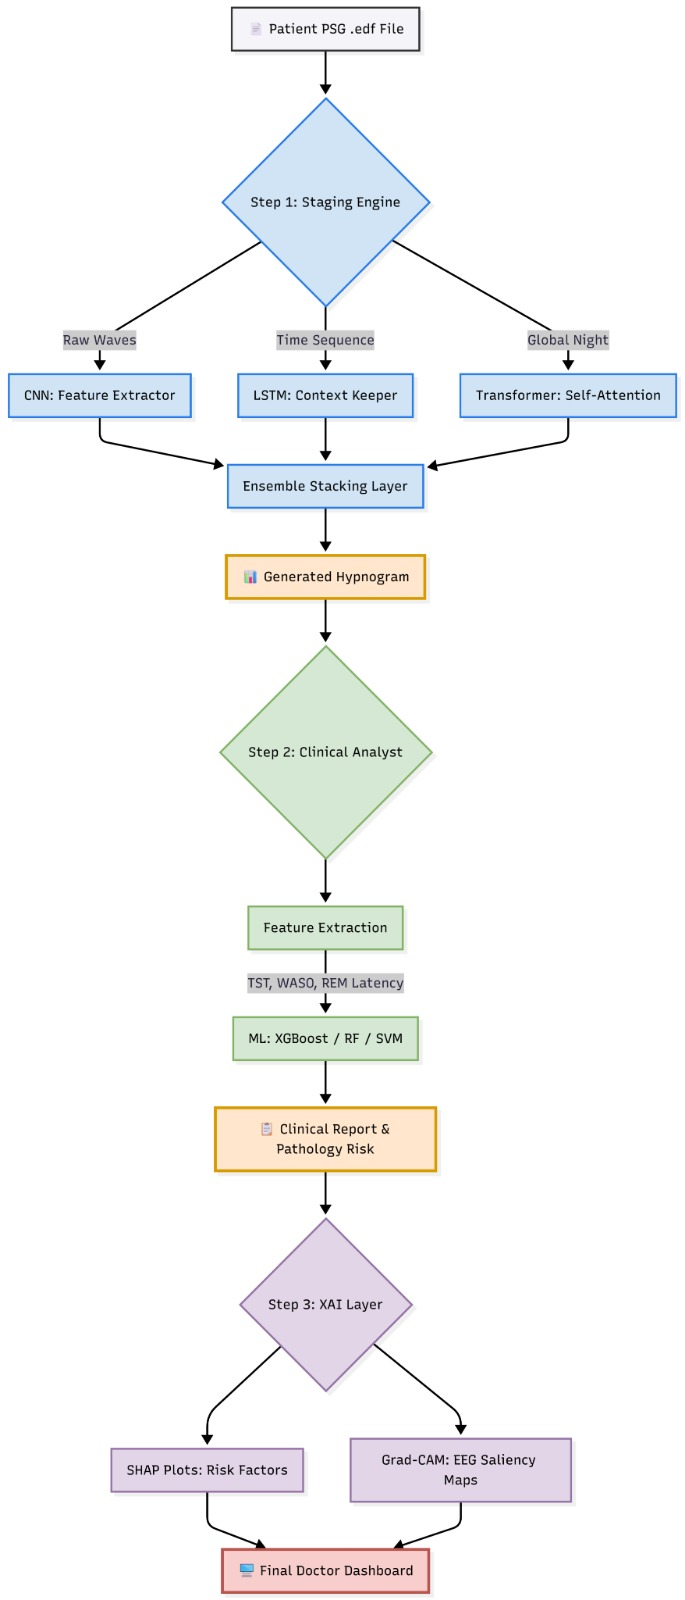
\includegraphics[height=0.78\textheight,keepaspectratio]{images/architecture.jpeg}
\caption[Architecture fonctionnelle du pipeline d'analyse]%
        {Pipeline d'analyse en trois étapes : classification des stades, analyse
         clinique et explication des décisions.}
\label{fig:pipeline}
\end{figure}

\subsection{Architecture physique}

La figure~\ref{fig:deploiement} décrit la topologie d'exécution. Chaque service est
conteneurisé et l'ensemble démarre par une commande unique. Le service de stockage est
le seul élément externe à l'infrastructure.

\begin{figure}[H]
\centering
\begin{tikzpicture}[
    x=1cm,y=1cm,
    noeud/.style  = {rectangle,rounded corners=3pt,draw=hypnoblue!55,fill=white,
                     align=center,font=\scriptsize,minimum height=1.5cm,
                     text width=3.2cm},
    hote/.style   = {rectangle,rounded corners=3pt,draw=hypnogray!55,dashed,
                     fill=hypnolight!35},
    cloud/.style  = {rectangle,rounded corners=8pt,draw=hypnogray!65,fill=white,
                     align=center,font=\scriptsize,minimum height=1.5cm,
                     text width=3.0cm},
    fl/.style     = {-{Latex[length=2mm]},hypnoblue!75,line width=0.8pt},
    lab/.style    = {font=\tiny\itshape,text=hypnogray,fill=white,inner sep=1.5pt},
  ]

  \node[hote,minimum width=11.4cm,minimum height=2.5cm] at (5.7,0) {};
  \node[font=\scriptsize\bfseries,text=hypnogray,anchor=north west] at (0.15,1.15)
       {Hôte de déploiement --- orchestration de conteneurs};

  \node[noeud] (front) at (2.1,-0.2)  {\textbf{Serveur web}\\\tiny Nginx\\\tiny
                                        application compilée};
  \node[noeud] (back)  at (5.7,-0.2)  {\textbf{Interface applicative}\\\tiny Uvicorn
                                        et FastAPI\\\tiny modèles en mémoire};
  \node[noeud] (db)    at (9.3,-0.2)  {\textbf{Base de données}\\\tiny PostgreSQL\\
                                        \tiny volume persistant};

  \node[cloud] (b2)    at (13.6,-0.2) {\textbf{Stockage objet}\\\tiny service externe\\
                                        \tiny interface S3};

  \node[font=\scriptsize\bfseries,align=center,text width=2.2cm] (nav) at (2.1,2.35)
       {Navigateur\\du praticien};

  \draw[fl] (nav) -- node[lab] {HTTPS} (front);
  \draw[fl] (front) -- node[lab] {mandataire} (back);
  \draw[fl] (back) -- node[lab] {SQL} (db);
  \draw[fl] (back) -- node[lab] {S3} (b2);

\end{tikzpicture}
\vspace{0.3cm}
\caption[Vue de déploiement]%
        {Topologie d'exécution : trois conteneurs sur un hôte, un service de stockage
         externe.}
\label{fig:deploiement}
\end{figure}

\section{Planification des releases}
\label{sec:planification}

\subsection{Découpage en releases}

Une release est une version livrable du produit : elle regroupe plusieurs sprints autour
d'un objectif de valeur commun et se clôt par une revue au cours de laquelle l'incrément est
démontré dans son ensemble. Le backlog du produit a été ordonnancé en trois releases de deux
sprints chacune, présentées au tableau~\ref{tab:releases} et à la figure~\ref{fig:releases}.

\begin{table}[H]
\centering

\small
\begin{tabular}{@{}L{2.5cm}L{2.2cm}L{4.5cm}L{3.8cm}c@{}}
\toprule
\textbf{Release} & \textbf{Sprints} & \textbf{Objectif} & \textbf{Incrément livrable} &
\textbf{Pts} \\
\midrule
\textbf{R1}\newline Moteur de classification & S1 et S2\newline du 26 jan.\newline au 22 mars &
Constituer le corpus et entraîner les modèles de classification des stades &
Corpus étiqueté et douze modèles de base évalués & 76 \\
\addlinespace[3pt]
\textbf{R2}\newline Diagnostic expliqué & S3 et S4\newline du 23 mars\newline au 17 mai &
Livrer au praticien un diagnostic expliqué à partir d'un enregistrement brut &
Ensembles, modèle de sévérité expliqué, interface applicative et poste de travail & 122 \\
\addlinespace[3pt]
\textbf{R3}\newline Plateforme clinique & S5 et S6\newline du 18 mai\newline au 12 juil. &
Faire de l'outil d'analyse une plateforme gouvernée, collaborative et déployable &
Dossier patient, archivage, administration, collaboration, compte rendu, pile
conteneurisée & 160 \\
\bottomrule
\end{tabular}
\caption{Planification du projet en trois releases}
\label{tab:releases}
\end{table}

L'ordre des releases découle des dépendances entre récits et de la répartition de
l'incertitude. La première traite en priorité ce qui était à la fois le plus incertain et le
plus structurant : le moteur de classification, dont dépend tout le reste. La deuxième livre
le plus petit incrément porteur de la valeur centrale du projet, un diagnostic expliqué
accessible au praticien. La troisième ajoute ce qui rend cet outil exploitable durablement
et à plusieurs : dossier patient, gouvernance, collaboration et déploiement reproductible.

\begin{figure}[H]
\centering
\begin{tikzpicture}[
    x=1cm,y=1cm,
    rel/.style = {rectangle,rounded corners=3pt,draw=hypnoblue!55,fill=hypnolight,
                  minimum width=4.9cm,minimum height=2.9cm},
    spr/.style = {rectangle,rounded corners=2pt,draw=hypnoblue!70,fill=white,
                  align=center,font=\scriptsize,minimum height=1.05cm,text width=1.85cm},
    tit/.style = {font=\scriptsize,text=hypnoblue,align=center,text width=4.6cm},
    liv/.style = {font=\scriptsize\itshape,text=hypnogray,align=center,text width=4.7cm},
    jal/.style = {diamond,fill=hypnored,draw=hypnored!85,inner sep=1.8pt},
    sem/.style = {font=\tiny,text=hypnogray},
    axe/.style = {-{Latex[length=2.2mm]},hypnogray!70,line width=0.8pt},
  ]

  % Axe du temps et livraisons
  \draw[axe] (0,1.95) -- (15.85,1.95);
  \node[sem,anchor=south west] at (0,2.05)    {semaine 1};
  \node[jal] at (4.9,1.95)  {};
  \node[sem,anchor=south] at (4.9,2.08)       {semaine 8};
  \node[jal] at (10.3,1.95) {};
  \node[sem,anchor=south] at (10.3,2.08)      {semaine 16};
  \node[jal] at (15.7,1.95) {};
  \node[sem,anchor=south east] at (15.8,2.08) {semaine 24};

  % Release 1
  \node[rel] at (2.45,0) {};
  \node[tit,anchor=north] at (2.45,1.35) {\textbf{Release 1}\\ moteur de classification};
  \node[spr] at (1.3,-0.45)  {\textbf{Sprint 1}\\ préparation\\ des données\\ 29 pts};
  \node[spr] at (3.6,-0.45)  {\textbf{Sprint 2}\\ modèles de\\ classification\\ 47 pts};
  \node[liv,anchor=north] at (2.45,-1.6) {corpus étiqueté et douze modèles évalués};

  % Release 2
  \node[rel] at (7.85,0) {};
  \node[tit,anchor=north] at (7.85,1.35) {\textbf{Release 2}\\ diagnostic expliqué};
  \node[spr] at (6.7,-0.45)  {\textbf{Sprint 3}\\ ensembles et\\ sévérité\\ 42 pts};
  \node[spr] at (9.0,-0.45)  {\textbf{Sprint 4}\\ service et\\ interface\\ 80 pts};
  \node[liv,anchor=north] at (7.85,-1.6) {premier diagnostic expliqué\\ accessible au praticien};

  % Release 3
  \node[rel] at (13.25,0) {};
  \node[tit,anchor=north] at (13.25,1.35) {\textbf{Release 3}\\ plateforme clinique};
  \node[spr] at (12.1,-0.45) {\textbf{Sprint 5}\\ dossier et\\ gouvernance\\ 77 pts};
  \node[spr] at (14.4,-0.45) {\textbf{Sprint 6}\\ collaboration,\\ déploiement\\ 83 pts};
  \node[liv,anchor=north] at (13.25,-1.6) {plateforme complète et conteneurisée};

\end{tikzpicture}
\vspace{0.2cm}
\caption[Feuille de route des releases]%
        {Feuille de route du projet : trois releases de deux sprints, chacune close par la
         livraison d'un incrément.}
\label{fig:releases}
\end{figure}

\subsection{Découpage en sprints}

Les vingt-six semaines du stage ont été découpées en six sprints de quatre semaines, suivis
de deux semaines consacrées à la rédaction et à la préparation de la soutenance. Le
tableau~\ref{tab:sprints} présente l'objectif et le livrable de chacun, regroupés par
release.

\begin{table}[H]
\centering

\small
\begin{tabular}{@{}L{1.5cm}L{2.5cm}L{5.0cm}L{4.4cm}c@{}}
\toprule
\textbf{Sprint} & \textbf{Période} & \textbf{Objectif} & \textbf{Livrable} &
\textbf{Pts} \\
\midrule
\multicolumn{5}{@{}l}{\cellcolor{hypnolight}\textbf{Release 1 --- Moteur de classification des stades}}\\
\midrule
S1 & 26 jan.\newline 22 fév. &
Cadrer le projet, lancer la demande d'accès aux cohortes et prouver la faisabilité de
la chaîne sans attendre l'autorisation &
Chaîne de prétraitement opérationnelle et premiers modèles de faisabilité & 29 \\
\addlinespace[3pt]
S2 & 23 fév.\newline 22 mars &
Passer du jeu d'amorçage à la cohorte clinique et couvrir les trois familles
d'architectures &
Douze modèles de base entraînés et évalués & 47 \\
\epictitre{Release 2 --- Diagnostic expliqué et poste de travail}
S3 & 23 mars\newline 19 avr. &
Faire coopérer les architectures, puis franchir le pas du staging vers le diagnostic
expliqué &
Quatre ensembles et le modèle de sévérité avec ses explications & 42 \\
\addlinespace[3pt]
S4 & 20 avr.\newline 17 mai &
Rendre les modèles consommables et donner au praticien un parcours guidé &
API documentée et parcours complet du dépôt au compte rendu & 80 \\
\epictitre{Release 3 --- Plateforme clinique et industrialisation}
S5 & 18 mai\newline 14 juin &
Transformer l'outil d'analyse en plateforme gouvernée et traçable &
Dossier patient persistant, archivage cloud, espace d'administration & 77 \\
\addlinespace[3pt]
S6 & 15 juin\newline 12 juil. &
Couvrir le travail à plusieurs, la restitution documentaire et la reproductibilité &
Collaboration, compte rendu exportable, pile conteneurisée & 83 \\
\bottomrule
\end{tabular}
\caption{Découpage des releases en sprints}
\label{tab:sprints}
\end{table}

\subsection{Vélocité}

La vélocité mesure le nombre de points effectivement livrés par sprint. Sa progression,
représentée à la figure~\ref{fig:velocite}, ne décrit pas un plateau régulier, ce qui
correspond à la réalité du travail : les deux premiers sprints sont absorbés par la
montée en compétence sur le cadre d'apprentissage profond et par des temps
d'entraînement incompressibles.

Regroupée par release, la vélocité moyenne passe de 38 points par sprint pour la
première à 61 pour la deuxième et 80 pour la troisième. Ce profil reflète la nature des
releases : la première est dominée par la modélisation, les suivantes par le
développement applicatif, moins exposé aux temps de calcul.

\begin{figure}[H]
\centering
\begin{tikzpicture}[x=1cm,y=1cm]

  % Axe des ordonnées
  \draw[hypnogray!60,line width=0.6pt] (0,0) -- (0,4.6);
  \foreach \v/\y in {0/0, 20/1.0, 40/2.0, 60/3.0, 80/4.0} {
    \draw[hypnogray!60] (-0.1,\y) -- (0,\y);
    \node[left,font=\scriptsize,text=hypnogray] at (-0.12,\y) {\v};
    \draw[hypnogray!18,line width=0.4pt] (0,\y) -- (10.6,\y);
  }
  \node[rotate=90,font=\scriptsize,text=hypnogray] at (-1.0,2.3) {points livrés};

  % Barres
  \foreach \i/\lab/\pts/\col in {0/S1/29/hypnoblue!40, 1/S2/47/hypnoblue!40,
      2/S3/42/hypnoblue!65, 3/S4/80/hypnoblue!65, 4/S5/77/hypnoblue!90, 5/S6/83/hypnoblue!90} {
    \pgfmathsetmacro{\xa}{0.55 + \i*1.65}
    \pgfmathsetmacro{\xb}{\xa + 1.1}
    \pgfmathsetmacro{\hh}{\pts/20}
    \fill[\col] (\xa,0) rectangle (\xb,\hh);
    \draw[hypnoblue] (\xa,0) rectangle (\xb,\hh);
    \node[font=\scriptsize\bfseries,text=hypnoblue,anchor=south]
         at ({(\xa+\xb)/2},\hh+0.04) {\pts};
    \node[font=\scriptsize,text=hypnogray,anchor=north]
         at ({(\xa+\xb)/2},-0.06) {\lab};
  }

  % Axe des abscisses
  \draw[hypnogray!60,line width=0.6pt] (0,0) -- (10.6,0);

  % Regroupement par release
  \foreach \r/\xa/\xb in {1/0.55/3.30, 2/3.85/6.60, 3/7.15/9.90} {
    \draw[hypnogray!70,line width=0.5pt] (\xa,-0.42) -- (\xa,-0.52) -- (\xb,-0.52)
          -- (\xb,-0.42);
    \node[font=\scriptsize\bfseries,text=hypnoblue,anchor=north]
         at ({(\xa+\xb)/2},-0.56) {Release \r};
  }

  % Vélocité moyenne
  \draw[hypnored,dashed,line width=0.8pt] (0,2.983) -- (10.6,2.983);
  \node[font=\scriptsize\itshape,text=hypnored,anchor=west] at (10.65,2.983)
       {moyenne : 60};

\end{tikzpicture}
\vspace{0.3cm}
\caption[Vélocité par sprint]%
        {Points de complexité livrés par sprint, regroupés par release.}
\label{fig:velocite}
\end{figure}

\subsection{Planning}

La figure~\ref{fig:gantt} confronte la planification aux travaux réellement menés. Le
jalon le plus structurant est l'obtention de l'accès aux cohortes en semaine 5. Le
recouvrement volontaire entre la demande d'accès et les travaux d'amorçage sur un jeu
public traduit une décision assumée : occuper le délai administratif au lieu de le
subir.

\begin{figure}[H]
\centering
\begin{ganttchart}[
    x unit                  = 0.375cm,
    y unit title            = 0.52cm,
    y unit chart            = 0.44cm,
    hgrid                   = {draw=hypnogray!18},
    vgrid                   = {*1{draw=hypnogray!18}},
    title/.append style     = {draw=hypnoblue!45, fill=hypnolight},
    title label font        = \tiny,
    title height            = 1,
    bar/.append style       = {draw=hypnoblue!85, fill=hypnoblue!55,
                               rounded corners=1pt},
    bar height              = 0.58,
    bar label font          = \scriptsize,
    bar label node/.append style = {text=hypnoblue!95},
    milestone/.append style = {fill=hypnored, draw=hypnored!85},
    milestone label font    = \scriptsize\itshape,
    milestone label node/.append style = {text=hypnored},
    milestone height        = 0.42,
  ]{1}{26}

  \gantttitle{Release 1}{8}
  \gantttitle{Release 2}{8}
  \gantttitle{Release 3}{8}
  \gantttitle{}{2} \\
  \gantttitle{Sprint 1}{4}
  \gantttitle{Sprint 2}{4}
  \gantttitle{Sprint 3}{4}
  \gantttitle{Sprint 4}{4}
  \gantttitle{Sprint 5}{4}
  \gantttitle{Sprint 6}{4}
  \gantttitle{Clôture}{2} \\
  \gantttitlelist{1,...,26}{1} \\

  \ganttbar{Étude bibliographique}{1}{3} \\
  \ganttbar{Demande d'accès NSRR}{1}{5} \\
  \ganttbar{Chaîne de prétraitement}{2}{4} \\
  \ganttbar{Amorçage sur jeu public}{3}{4} \\
  \ganttmilestone{Accès aux cohortes obtenu}{5} \\
  \ganttbar{Préparation de la cohorte}{5}{6} \\
  \ganttbar{Modèles de base}{6}{9} \\
  \ganttmilestone{12 modèles entraînés}{9} \\
  \ganttbar{Ensembles par empilement}{9}{10} \\
  \ganttbar{Modèle de sévérité}{10}{12} \\
  \ganttbar{Service d'inférence}{13}{15} \\
  \ganttbar{Interface d'analyse}{14}{17} \\
  \ganttbar{Base de données, archivage}{17}{19} \\
  \ganttbar{Administration, audit}{19}{20} \\
  \ganttbar{Collaboration, annotation}{21}{22} \\
  \ganttbar{Compte rendu, multilinguisme}{22}{23} \\
  \ganttmilestone{Plateforme complète}{22} \\
  \ganttbar{Conteneurisation, intégration}{23}{24} \\
  \ganttbar{Rédaction du mémoire}{21}{26} \\
  \ganttmilestone{Soutenance}{26}

\end{ganttchart}
\vspace{0.3cm}
\caption[Diagramme de Gantt du projet]%
        {Déroulement du projet sur les vingt-six semaines du stage.}
\label{fig:gantt}
\end{figure}

\sectionsansnum{Conclusion}

Ce chapitre a traduit les intentions du chapitre précédent en une commande vérifiable.
Quatre acteurs ont été identifiés, les besoins fonctionnels regroupés en neuf épics et
déclinés en soixante récits utilisateur, et les besoins non fonctionnels énoncés avec
leur moyen de vérification. Le modèle de données, l'environnement de travail et
l'architecture globale ont été présentés.

L'ordonnancement du backlog a produit trois releases de deux sprints de quatre semaines.
Les trois chapitres suivants leur sont consacrés. Chacun suit la même trame : présentation
de la release et de son backlog ; pour chaque sprint, backlog, analyse, conception,
réalisation et revue ; enfin, revue de la release.
    % Analyse, specification et planification des releases
\chapter{Release 1 : Moteur de classification des stades}
\label{chap:release1}

\sectionsansnum{Introduction}

Ce chapitre rend compte de la première release de \hypnoria{}, menée de la semaine 1 à la
semaine 8 du stage. Son enjeu est de constituer le socle sur lequel repose tout le reste du
système : un corpus d'apprentissage homogène et des modèles capables de classer
automatiquement les stades du sommeil. Après avoir présenté l'objectif et le backlog de la
release, nous détaillons ses deux sprints (la préparation des données, puis
l'entraînement des modèles) avant d'en dresser la revue.

% ---------------------------------------------------------------------------
\section{Présentation de la release}
\label{sec:release1}
% ---------------------------------------------------------------------------

\subsection{Objectif de la release}

La première release vise à livrer un moteur de classification des stades validé.
Aucune fonctionnalité n'y est encore accessible au praticien : l'incrément attendu est un
ensemble de modèles entraînés et évalués, dont dépend la valeur de toutes les releases
suivantes.

Placer ce moteur en tête de la planification répond à la logique de réduction de
l'incertitude exposée au chapitre~\ref{chap:presentation}. C'est ici que se concentraient
les deux incertitudes majeures du projet : le délai d'accès aux cohortes cliniques et le
niveau de performance effectivement atteignable. Les lever en premier évitait de construire
une plateforme autour de modèles dont rien ne garantissait encore la qualité.

\subsection{Backlog de la release}

La release regroupe les huit premiers récits du backlog, ceux de l'épic E1, pour
76 points de complexité
répartis sur deux sprints de quatre semaines (tableau~\ref{tab:rel1}).

\begin{table}[H]
\centering\small
\renewcommand{\arraystretch}{1.2}
\begin{tabular}{@{}L{1.4cm}|L{3.0cm}|L{5.4cm}|L{2.7cm}|c@{}}
\hline
\ligneentete \entete{Sprint} & \entete{Période} & \entete{Objectif du sprint} &
\entete{Récits} & \entete{Pts} \\
\hline
Sprint 1 & 26 jan. -- 22 fév. &
Construire la chaîne de préparation du signal et la valider sur un jeu public &
US-01 à 04 & 29 \\
\hline
Sprint 2 & 23 fév. -- 22 mars &
Préparer la cohorte clinique et entraîner les trois familles d'architectures &
US-05 à 08 & 47 \\
\hline
\multicolumn{3}{@{}r|}{\textbf{Total de la release}} & \textbf{8 récits} & \textbf{76} \\
\hline
\end{tabular}
\caption{Backlog de la release 1}
\label{tab:rel1}
\end{table}

\noindent
L'incrément attendu en fin de release comprend un corpus d'apprentissage étiqueté conforme
au référentiel AASM et douze modèles de base couvrant trois architectures, deux montages et
deux granularités.

% ---------------------------------------------------------------------------
\section{Sprint 1 : Préparation des données et amorçage}
\label{sec:sprint1}
% ---------------------------------------------------------------------------

Ce premier sprint est consacré à la constitution du corpus d'apprentissage. La qualité
des modèles dépend d'abord de celle des données : avant toute architecture, il fallait
transformer des enregistrements bruts hétérogènes en un corpus homogène et étiqueté. Le
sprint s'est heurté à une contrainte externe, le délai d'instruction de la demande
d'accès aux cohortes cliniques, que nous avons choisi d'occuper plutôt que de subir.

\subsection{Objectif du sprint}

L'objectif était double. Il s'agissait d'abord de construire la chaîne de
préparation du signal : lire un fichier au format EDF quel que soit son constructeur,
en extraire les cinq dérivations utiles, uniformiser la fréquence d'échantillonnage,
découper le signal en fenêtres conformes au référentiel AASM et neutraliser les écarts
d'amplitude entre sujets.

Il s'agissait ensuite de valider cette chaîne de bout en bout sans attendre
l'autorisation d'accès aux cohortes du \emph{National Sleep Research
Resource}~\cite{zhang2018nsrr}, dont l'instruction prend plusieurs semaines. Le jeu
public Sleep-EDF~\cite{kemp2000}, diffusé par PhysioNet~\cite{goldberger2000} et
immédiatement téléchargeable, a servi de banc d'essai.

Ce choix constitue le principal arbitrage de gestion de projet du stage. Attendre
l'autorisation aurait immobilisé quatre semaines. Travailler
sur un jeu public de substitution permettait de valider la lecture des fichiers, la
résolution des dérivations, la segmentation et la boucle d'entraînement avant même de
disposer des données définitives. Lorsque l'autorisation est arrivée en semaine 5, la
chaîne était éprouvée et il n'a plus été question que de la rejouer à plus grande
échelle.

\subsection{Sprint Backlog}

Le sprint a embarqué quatre récits utilisateur pour un total de 29 points de
complexité, détaillés au tableau~\ref{tab:bl-s1}.

\begin{table}[H]
\centering\small
\renewcommand{\arraystretch}{1.15}
\begin{tabular}{@{}c|L{2.5cm}|L{4.6cm}|L{4.6cm}|c@{}}
\hline
\ligneentete \entete{ID} & \entete{Module} & \entete{R\'ecit utilisateur} & \entete{T\^aches} & \entete{Estim.} \\
\hline
\multirow{3}{*}{US-01} & \multirow{3}{=}{Lecture des enregistrements} & \multirow{3}{=}{En tant que syst\`eme, je veux lire un fichier EDF et en extraire les d\'erivations physiologiques} & Int\'egrer la biblioth\`eque de lecture des formats physiologiques & \multirow{3}{*}{8 pts} \\
 &  &  & Inventorier les d\'erivations et la fr\'equence native &  \\
 &  &  & G\'erer les fichiers tronqu\'es ou illisibles &  \\
\hline
\multirow{3}{*}{US-02} & \multirow{3}{=}{R\'esolution des canaux} & \multirow{3}{=}{En tant que syst\`eme, je veux r\'esoudre les canaux malgr\'e l'h\'et\'erog\'en\'eit\'e des conventions de nommage} & Construire la table d'alias des cinq emplacements logiques & \multirow{3}{*}{5 pts} \\
 &  &  & D\'efinir la strat\'egie de repli sur l'EEG principal &  \\
 &  &  & Exiger le montage complet \`a l'entra\^inement &  \\
\hline
\multirow{4}{*}{US-03} & \multirow{4}{=}{Normalisation du signal} & \multirow{4}{=}{En tant que syst\`eme, je veux r\'e\'echantillonner, segmenter en \'epoques de 30 s et normaliser} & R\'e\'echantillonner \`a 100\,Hz par m\'ethode de Fourier & \multirow{4}{*}{8 pts} \\
 &  &  & D\'ecouper en fen\^etres de 3\,000 \'echantillons &  \\
 &  &  & Centrer et r\'eduire chaque fen\^etre &  \\
 &  &  & S\'erialiser en tenseurs par sujet &  \\
\hline
\multirow{3}{*}{US-04} & \multirow{3}{=}{Amor\c{c}age} & \multirow{3}{=}{En tant qu'ing\'enieur, je veux valider la cha\^ine sur un jeu public avant l'acc\`es aux cohortes cliniques} & T\'el\'echarger et pr\'eparer le jeu public & \multirow{3}{*}{8 pts} \\
 &  &  & Entra\^iner un mod\`ele de faisabilit\'e &  \\
 &  &  & V\'erifier la boucle compl\`ete de bout en bout &  \\
\hline
\end{tabular}
\caption{Sprint Backlog --- Sprint 1}
\label{tab:bl-s1}
\end{table}

\subsection{Analyse}

\subsubsection{Diagramme des cas d'utilisation}

Ce sprint ne produit pas de fonctionnalité directement visible par le praticien : il
construit le socle sur lequel reposeront tous les suivants. Le cas d'utilisation
principal est donc porté par le moteur d'inférence, acteur secondaire du système
(figure~\ref{fig:uc-s1}).

\begin{figure}[H]
\centering
\begin{tikzpicture}[
    x=1cm,y=1cm,
    uc/.style     = {ellipse, draw=hypnoblue!60, fill=hypnolight,
                     align=center, font=\scriptsize, text width=2.6cm,
                     inner sep=1.5pt, minimum height=1.0cm},
    ucp/.style    = {ellipse, draw=hypnored!70, fill=hypnored!7,
                     align=center, font=\scriptsize\bfseries, text width=2.6cm,
                     inner sep=1.5pt, minimum height=1.0cm},
    lien/.style   = {hypnogray!75, line width=0.55pt},
    rel/.style    = {-{Latex[length=2mm]}, hypnoblue!70, line width=0.5pt, dashed},
    et/.style     = {font=\tiny\itshape, text=hypnoblue!85, fill=white, inner sep=1pt},
    nomact/.style = {font=\scriptsize\bfseries, align=center, text width=2.2cm},
  ]

  \tikzset{acteur/.pic={
      \draw[hypnoblue,line width=0.8pt] (0,0) circle (0.17);
      \draw[hypnoblue,line width=0.8pt] (0,-0.17) -- (0,-0.66);
      \draw[hypnoblue,line width=0.8pt] (-0.28,-0.34) -- (0.28,-0.34);
      \draw[hypnoblue,line width=0.8pt] (0,-0.66) -- (-0.24,-1.04);
      \draw[hypnoblue,line width=0.8pt] (0,-0.66) -- (0.24,-1.04);}}

  % Frontiere du systeme
  \draw[hypnoblue!55,line width=0.9pt,rounded corners=3pt]
       (3.1,-6.0) rectangle (12.5,2.4);
  \node[font=\small\bfseries,text=hypnoblue,anchor=north west] at (3.35,2.25)
       {Module de préparation des données};

  % Cas principal et cas terminal, colonne de gauche
  \node[ucp] (prep) at (5.1, 0.9)  {Préparer un\\enregistrement};
  \node[uc]  (ser)  at (5.1,-4.3)  {Sérialiser le\\corpus};

  % Sous-cas inclus, colonne de droite
  \node[uc]  (lire) at (10.0, 1.2) {Décoder le\\fichier EDF};
  \node[uc]  (res)  at (10.0,-0.3) {Résoudre les\\dérivations};
  \node[uc]  (ree)  at (10.0,-1.8) {Rééchantillonner\\à 100\,Hz};
  \node[uc]  (seg)  at (10.0,-3.3) {Segmenter en\\époques de 30\,s};
  \node[uc]  (nor)  at (10.0,-4.8) {Normaliser\\chaque époque};

  % Acteur
  \pic at (1.3,0.6) {acteur};
  \node[nomact,anchor=north] at (1.3,-0.05) {Moteur\\d'inférence};

  \draw[lien] (1.7,0.25) -- (prep.west);
  \draw[lien] (1.7,0.25) -- (ser.west);

  \draw[rel] (prep) -- node[et,pos=0.62] {$\ll$include$\gg$} (lire);
  \draw[rel] (prep) -- node[et,pos=0.62] {$\ll$include$\gg$} (res);
  \draw[rel] (prep) -- node[et,pos=0.62] {$\ll$include$\gg$} (ree);
  \draw[rel] (prep) -- node[et,pos=0.66] {$\ll$include$\gg$} (seg);
  \draw[rel] (prep) -- node[et,pos=0.70] {$\ll$include$\gg$} (nor);

\end{tikzpicture}
\caption{Diagramme des cas d'utilisation du sprint 1 --- préparation des données}
\label{fig:uc-s1}
\end{figure}

\subsubsection{Description textuelle des cas d'utilisation}

\begin{casutilisation}{Description textuelle du cas « Préparer un enregistrement »}
Titre & Préparer un enregistrement \\ \hline
Acteur & Moteur d'inférence \\ \hline
Description & Transformer un enregistrement polysomnographique brut en un ensemble de
fenêtres normalisées, directement exploitables par un modèle de classification \\ \hline
Préconditions & Un fichier au format EDF est disponible et lisible \\ \hline
Scénario de base &
\begin{minipage}[t]{\linewidth}
\begin{enumerate}[leftmargin=1.1em,itemsep=1pt,topsep=3pt]
  \item Le système décode le fichier et inventorie ses dérivations.
  \item Il apparie chaque dérivation attendue à son équivalent dans le fichier.
  \item Il ramène l'ensemble des signaux à \SI{100}{\hertz}.
  \item Il découpe le signal en fenêtres de \num{3000} échantillons.
  \item Il centre et réduit chaque fenêtre indépendamment.
  \item Il sérialise le résultat sous forme de tenseur accompagné de ses étiquettes.
\end{enumerate}
\end{minipage} \\ \hline
Scénario alternatif &
\begin{minipage}[t]{\linewidth}
\begin{itemize}[leftmargin=1.1em,itemsep=1pt,topsep=3pt]
  \item \textbf{2a} --- Une dérivation est absente : en production, repli documenté sur
        l'EEG principal ; à l'entraînement, le sujet est écarté du corpus.
  \item \textbf{4a} --- L'enregistrement est plus court qu'une époque : le traitement
        s'interrompt avec un message explicite.
  \item \textbf{6a} --- L'hypnogramme de référence est absent : le sujet est écarté.
\end{itemize}
\end{minipage}
\end{casutilisation}

\subsection{Conception}

\subsubsection{Diagramme de séquence objet}

La figure~\ref{fig:seq-s1} détaille l'enchaînement des traitements appliqués à un
enregistrement.

\begin{figure}[H]
\centering
\resizebox{0.96\textwidth}{!}{%
\begin{sequencediagram}
  \newthread[hypnolight]{p}{\scriptsize Script de préparation}
  \newinst[2.0]{l}{\scriptsize Lecteur EDF}
  \newinst[2.0]{a}{\scriptsize Résolveur de canaux}
  \newinst[2.0]{s}{\scriptsize Traitement du signal}
  \newinst[2.0]{x}{\scriptsize Analyseur XML}
  \newinst[2.0]{f}{\scriptsize Corpus sérialisé}

  \begin{call}{p}{\scriptsize ouvrir l'enregistrement}{l}{\scriptsize dérivations, fréquence}
  \end{call}
  \begin{call}{p}{\scriptsize apparier les dérivations}{a}{\scriptsize table de correspondance}
  \end{call}
  \begin{sdblock}{\scriptsize Contrôle}{\scriptsize montage complet exigé}
    \begin{call}{p}{\scriptsize écarter le sujet si incomplet}{p}{}
    \end{call}
  \end{sdblock}
  \begin{call}{p}{\scriptsize rééchantillonner}{s}{\scriptsize signal à 100\,Hz}
  \end{call}
  \begin{call}{p}{\scriptsize lire l'hypnogramme}{x}{\scriptsize séquence de stades}
  \end{call}
  \begin{call}{p}{\scriptsize segmenter et normaliser}{s}{\scriptsize tenseur d'époques}
  \end{call}
  \begin{call}{p}{\scriptsize sérialiser}{f}{\scriptsize fichier par sujet}
  \end{call}
\end{sequencediagram}}
\caption{Diagramme de séquence objet du sprint 1 --- préparation d'un enregistrement}
\label{fig:seq-s1}
\end{figure}

\subsection{Réalisation}

\subsubsection{La chaîne de préparation}

La chaîne réalisée comporte six étapes, chacune répondant à une source de variabilité
identifiée (figure~\ref{fig:chaine}).

\begin{figure}[H]
\centering
\begin{tikzpicture}[
    x=1cm,y=1cm,
    et/.style  = {rectangle,rounded corners=2pt,draw=hypnoblue!60,fill=hypnolight,
                  align=center,font=\scriptsize,minimum height=1.25cm,
                  text width=2.15cm},
    fl/.style  = {-{Latex[length=2mm]},hypnoblue!75,line width=0.8pt},
    note/.style= {font=\tiny\itshape,text=hypnogray,align=center,text width=2.3cm},
  ]

  \node[et] (a) at (0.0,0)  {Décodage\\du fichier};
  \node[et] (b) at (2.75,0) {Résolution\\des dérivations};
  \node[et] (c) at (5.5,0)  {Rééchantillonnage\\à 100\,Hz};
  \node[et] (d) at (8.25,0) {Segmentation\\en époques};
  \node[et] (e) at (11.0,0) {Z-score\\par époque};
  \node[et] (f) at (13.75,0){Tenseur\\$(N, C, 3000)$};

  \foreach \x/\y in {a/b,b/c,c/d,d/e,e/f} \draw[fl] (\x) -- (\y);

  \node[note,anchor=north] at (0.0,-0.78)  {format\\constructeur};
  \node[note,anchor=north] at (2.75,-0.78) {conventions de\\nommage};
  \node[note,anchor=north] at (5.5,-0.78)  {fréquences\\d'acquisition};
  \node[note,anchor=north] at (8.25,-0.78) {convention\\AASM 30\,s};
  \node[note,anchor=north] at (11.0,-0.78) {amplitudes\\inter-sujets};
  \node[note,anchor=north] at (13.75,-0.78){entrée des\\modèles};

  \node[font=\tiny\bfseries,text=hypnored,anchor=east] at (-1.05,-1.35)
       {variabilité traitée :};

\end{tikzpicture}
\vspace{0.3cm}
\caption[Chaîne de traitement du signal]%
        {Chaîne de préparation : chaque étape neutralise une source de variabilité.}
\label{fig:chaine}
\end{figure}

Quatre décisions de traitement sont détaillées ci-dessous.

\subparagraph{Sélection stricte des dérivations.} À l'entraînement, les cinq dérivations
sont exigées sous leur dénomination exacte et tout écart écarte le sujet. En production,
au contraire, une table d'alias couvre les conventions de nommage des différents
constructeurs et replie sur l'EEG principal une dérivation absente. Cette asymétrie est
voulue : sélectivité pour la pureté du corpus d'apprentissage, tolérance pour
l'interopérabilité clinique. C'est un des rares endroits du système où une même fonction
est délibérément implémentée deux fois différemment.

\subparagraph{Fusion des anciens stades 3 et 4.} Les annotations des cohortes suivent
encore la nomenclature de Rechtschaffen et Kales~\cite{rechtschaffen1968}. Le stade 4
est fusionné dans le N3, conformément à la révision AASM de 2007.

\subparagraph{Comblement des époques non scorées.} Les fenêtres sans stade attribué
reçoivent le dernier stade valide observé ; celles qui précèdent le premier stade scoré
sont considérées comme de l'éveil. Cette dernière convention est une hypothèse
(l'enregistrement débute avant l'extinction des lumières) et non une donnée.

\subparagraph{Normalisation locale par z-score.} Chaque fenêtre est centrée sur sa
propre moyenne et réduite par son propre écart-type, dérivation par dérivation :

\[
  x'_{c,n}[k] \;=\; \frac{x_{c,n}[k] - \mu_{c,n}}{\sigma_{c,n} + \varepsilon},
  \qquad
  \mu_{c,n} = \frac{1}{K}\sum_{k=1}^{K} x_{c,n}[k],
  \qquad K = \num{3000},
\]

\noindent
où $\sigma_{c,n}$ est l'écart-type de la dérivation $c$ sur la fenêtre $n$ et
$\varepsilon = \num{1e-8}$ empêche la division par zéro lorsqu'une électrode s'est
détachée et que le segment est plat. Chaque fenêtre sort ainsi de moyenne nulle et de
variance unitaire, ce qui met les cinq dérivations sur une même échelle et évite que
l'EMG, physiquement plus faible, ne pèse rien devant l'EEG.

La statistique est donc calculée sur chaque fenêtre isolément, et non sur le corpus. Ce
choix neutralise les écarts d'amplitude liés à l'impédance des électrodes, au gain de
l'amplificateur et à la morphologie du sujet, ainsi que la dérive lente au cours de la
nuit. Il a surtout une conséquence méthodologique : aucune statistique globale n'étant
estimée, aucune information ne peut fuir de l'ensemble d'entraînement vers l'ensemble de
test par la normalisation. En contrepartie, l'information d'amplitude absolue est
perdue, alors qu'elle caractérise partiellement le sommeil profond.

\subsubsection{Le corpus produit}

La préparation est assurée par un script exécuté une seule fois, dont le produit
alimentera les douze entraînements du sprint suivant. Il prend en entrée les deux
fichiers que la cohorte livre pour chaque nuit : l'enregistrement au format EDF, qui
porte le signal, et un fichier XML d'annotations, qui porte le scorage de l'expert.

Du côté du signal, les cinq dérivations sont extraites sous leur nom exact, ramenées à
\SI{100}{\hertz} par rééchantillonnage de Fourier, découpées en fenêtres de \num{3000}
échantillons et centrées-réduites par z-score. Du côté des annotations, chaque élément
\texttt{ScoredEvent} de type « stades » donne un instant de début, une durée et un
stade ; le script les projette sur la grille de 30 secondes, replie le stade 4 sur le N3
et comble les fenêtres restées vides par le dernier stade valide. Les deux flux sont
ensuite alignés sur le plus court des deux, et les époques qu'aucun événement ne couvre
sont écartées.

Le résultat est sérialisé dans un fichier \texttt{.pt} par sujet, qui contient le
tenseur $X$ de forme $(N, 5, \num{3000})$ en simple précision, le vecteur d'étiquettes
$y$ en entier court, l'identifiant du sujet et son nombre d'époques. C'est cette
conversion qui rend l'entraînement possible sur le poste disponible. Seules les cinq
dérivations utiles sont conservées, à \SI{100}{\hertz} plutôt qu'à la fréquence
d'acquisition d'origine, et sans les voies respiratoires ni les canaux de service du
montage : la nuit tombe à environ \SI{60}{\mega\octet}. Le format y est aussi pour
quelque chose : le fichier est écrit exactement tel que le chargeur l'attend, si bien
que les douze entraînements du sprint suivant relisent le corpus sans repayer le
décodage EDF, le rééchantillonnage ni l'analyse du XML.

Le script est relançable : un sujet déjà converti est ignoré, ce qui permet
d'étaler la campagne de préparation sur plusieurs sessions et de rejouer la préparation
à l'identique.

Cent quatre-vingt-seize enregistrements de la cohorte SHHS1~\cite{quan1997} ont été
retenus, pour un total de \num{195130} époques de 30 secondes. Le
corpus est filtré et non échantillonné : un sujet est écarté s'il lui manque une
des cinq dérivations requises ou son fichier d'annotations. Les sujets retenus sont donc
les premiers de la cohorte à satisfaire le montage complet, ce qui introduit un biais de
sélection dont nous discuterons la portée.

\begin{figure}[H]
\centering
\begin{tikzpicture}[x=1cm,y=1cm]

  \def\W{11.4}

  % ── Barre 5 classes ───────────────────────────────────────────────────────
  \node[font=\scriptsize\bfseries,text=hypnogray,anchor=east] at (-0.25,1.55)
       {5 classes};
  \foreach \a/\b/\col/\lab/\pct in {
      0/30.70/stWake/W/30{,}7,
      30.70/33.96/stN1/N1/3{,}3,
      33.96/74.13/stN2/N2/40{,}2,
      74.13/87.09/stN3/N3/13{,}0,
      87.09/100/stREM/REM/12{,}9}
  {
    \pgfmathsetmacro{\xa}{\a*\W/100}
    \pgfmathsetmacro{\xb}{\b*\W/100}
    \pgfmathsetmacro{\xm}{(\xa+\xb)/2}
    \fill[\col!75] (\xa,1.15) rectangle (\xb,1.95);
    \draw[white,line width=0.8pt] (\xb,1.15) -- (\xb,1.95);
    \node[font=\tiny\bfseries,text=white] at (\xm,1.68) {\lab};
    \node[font=\tiny,text=white] at (\xm,1.40) {\pct\,\%};
  }

  % ── Barre 3 classes ───────────────────────────────────────────────────────
  \node[font=\scriptsize\bfseries,text=hypnogray,anchor=east] at (-0.25,0.35)
       {3 classes};
  \foreach \a/\b/\col/\lab/\pct in {
      0/30.70/stWake/Wake/30{,}7,
      30.70/87.09/stN2/NREM/56{,}4,
      87.09/100/stREM/REM/12{,}9}
  {
    \pgfmathsetmacro{\xa}{\a*\W/100}
    \pgfmathsetmacro{\xb}{\b*\W/100}
    \pgfmathsetmacro{\xm}{(\xa+\xb)/2}
    \fill[\col!75] (\xa,-0.05) rectangle (\xb,0.75);
    \draw[white,line width=0.8pt] (\xb,-0.05) -- (\xb,0.75);
    \node[font=\tiny\bfseries,text=white] at (\xm,0.48) {\lab};
    \node[font=\tiny,text=white] at (\xm,0.20) {\pct\,\%};
  }

  % ── Annotation ────────────────────────────────────────────────────────────
  \draw[hypnored,line width=0.7pt] (3.50,2.10) -- (3.50,2.45) -- (4.30,2.45);
  \node[font=\scriptsize,text=hypnored,anchor=west] at (4.35,2.45)
       {le N1 ne représente que \num{6361} époques sur \num{195130}};

  \node[font=\tiny\itshape,text=hypnogray,anchor=north] at (5.7,-0.35)
       {corpus SHHS1 --- 196 enregistrements, \num{195130} époques de 30 secondes};

\end{tikzpicture}
\vspace{0.35cm}
\caption[Distribution des stades dans le corpus SHHS1]%
        {Distribution des stades dans le corpus d'entraînement, aux deux granularités.}
\label{fig:distribution}
\end{figure}

Le déséquilibre conditionne tout le sprint suivant. Le N2 occupe à lui
seul \SI{40,2}{\percent} des époques, tandis que le N1 n'en représente que
\SI{3,3}{\percent}, soit \num{6361} exemples. Un modèle qui ignorerait purement et
simplement cette classe perdrait à peine trois points d'exactitude globale, comportement
que la pondération des classes doit empêcher.

\subsubsection{Découpage et pondération}

Le corpus est découpé en trois parts stratifiées sur la classe, dans les proportions
\num{80} / \num{10} / \num{10}, soit \num{156104} époques d'entraînement et \num{19513}
pour chacun des ensembles de validation et de test. La pondération des classes est fixée
à l'inverse de leur fréquence, puis renormalisée : le REM se voit attribuer un poids
\num{4,4} fois supérieur à celui du NREM en trois classes, et le N1 un poids \num{12,3}
fois supérieur à celui du N2 en cinq classes.

\subsection{Revue du sprint}

Ce premier sprint a produit le socle de tout le projet : une chaîne de préparation
opérationnelle et un corpus de \num{195130} époques étiquetées, issues de 196
enregistrements cliniques.

L'arbitrage de départ, travailler sur un jeu public pendant l'instruction de la
demande d'accès, s'est révélé payant : lorsque les données définitives sont arrivées,
la chaîne était éprouvée et il n'a suffi que de la rejouer à plus grande échelle.

Deux constats issus de ce sprint pèseront sur les suivants : le corpus est fortement
déséquilibré, avec un stade N1 marginal, et il résulte d'un filtrage sur la complétude
du montage plutôt que d'un tirage aléatoire. Le sprint suivant exploite ce corpus pour
entraîner les trois familles d'architectures de classification.

% ---------------------------------------------------------------------------
\section{Sprint 2 : Modèles de classification des stades}
\label{sec:sprint2}
% ---------------------------------------------------------------------------

Le deuxième sprint est consacré à l'entraînement des modèles de classification. Le corpus
produit au sprint précédent y est exploité pour entraîner trois familles d'architectures sur
quatre configurations, soit douze modèles au total. Le sprint a été dominé par une contrainte
matérielle qui a imposé un arbitrage explicite sur la quantité de données exploitable, et
dont la portée conditionne la lecture de tous les résultats.

\subsection{Objectif du sprint}

L'objectif était de couvrir les trois familles d'architectures identifiées
comme complémentaires dans l'étude préalable, sur les quatre configurations
retenues : deux montages (cinq dérivations pour le laboratoire, deux pour
l'ambulatoire) et deux granularités de sortie (trois stades pour la robustesse,
cinq pour la conformité au référentiel AASM).

Ce plan factoriel répond à une question que la littérature laisse
généralement ouverte : quelle est la part respective, dans la performance finale, de
l'architecture du modèle, du nombre de dérivations disponibles et de la granularité
demandée ? Entraîner les douze combinaisons permet d'y répondre par comparaison directe,
sur un protocole identique.

\subsection{Sprint Backlog}

Le sprint a embarqué quatre récits pour 47 points de complexité
(tableau~\ref{tab:bl-s2}).

\begin{table}[H]
\centering\small
\renewcommand{\arraystretch}{1.15}
\begin{tabular}{@{}c|L{2.5cm}|L{4.6cm}|L{4.6cm}|c@{}}
\hline
\ligneentete \entete{ID} & \entete{Module} & \entete{R\'ecit utilisateur} & \entete{T\^aches} & \entete{Estim.} \\
\hline
\multirow{3}{*}{US-05} & \multirow{3}{=}{Corpus \`a l'\'echelle} & \multirow{3}{=}{En tant qu'ing\'enieur, je veux pr\'etraiter les 196 enregistrements de la cohorte clinique} & Rapatrier la cohorte apr\`es obtention de l'acc\`es & \multirow{3}{*}{8 pts} \\
 &  &  & Rejouer la cha\^ine de pr\'eparation \`a l'\'echelle &  \\
 &  &  & Contr\^oler la distribution des classes obtenue &  \\
\hline
\multirow{3}{*}{US-06} & \multirow{3}{=}{R\'eseau convolutif} & \multirow{3}{=}{En tant que syst\`eme, je veux classer chaque \'epoque avec un r\'eseau convolutif multi-\'echelle} & Concevoir les deux branches d'\'echelles distinctes & \multirow{3}{*}{13 pts} \\
 &  &  & Impl\'ementer la boucle d'entra\^inement &  \\
 &  &  & Entra\^iner les quatre variantes &  \\
\hline
\multirow{3}{*}{US-07} & \multirow{3}{=}{R\'eseau r\'ecurrent} & \multirow{3}{=}{En tant que syst\`eme, je veux classer chaque \'epoque avec un r\'eseau r\'ecurrent \`a pooling attentionnel} & Impl\'ementer le r\'eseau bidirectionnel \`a m\'emoire longue & \multirow{3}{*}{13 pts} \\
 &  &  & Ajouter le m\'ecanisme d'attention temporelle &  \\
 &  &  & Entra\^iner les quatre variantes &  \\
\hline
\multirow{3}{*}{US-08} & \multirow{3}{=}{R\'eseau attentionnel} & \multirow{3}{=}{En tant que syst\`eme, je veux classer chaque \'epoque avec un Transformer par patchs} & D\'ecouper l'\'epoque en fragments et les projeter & \multirow{3}{*}{13 pts} \\
 &  &  & Ajouter le jeton de synth\`ese et l'encodage positionnel &  \\
 &  &  & Entra\^iner les quatre variantes &  \\
\hline
\end{tabular}
\caption{Sprint Backlog --- Sprint 2}
\label{tab:bl-s2}
\end{table}

\subsection{Analyse}

\subsubsection{Diagramme des cas d'utilisation}

Le cas d'utilisation de ce sprint reste porté par le moteur d'inférence
(figure~\ref{fig:uc-s2}). Le praticien n'y accède pas directement : il en bénéficiera au
sprint~4, dans la release~2, lorsque le service d'inférence sera exposé.

\begin{figure}[H]
\centering
\begin{tikzpicture}[
    x=1cm,y=1cm,
    uc/.style     = {ellipse, draw=hypnoblue!60, fill=hypnolight,
                     align=center, font=\scriptsize, text width=2.7cm,
                     inner sep=1.5pt, minimum height=1.0cm},
    ucp/.style    = {ellipse, draw=hypnored!70, fill=hypnored!7,
                     align=center, font=\scriptsize\bfseries, text width=2.7cm,
                     inner sep=1.5pt, minimum height=1.0cm},
    lien/.style   = {hypnogray!75, line width=0.55pt},
    rel/.style    = {-{Latex[length=2mm]}, hypnoblue!70, line width=0.5pt, dashed},
    et/.style     = {font=\tiny\itshape, text=hypnoblue!85, fill=white, inner sep=1pt},
    nomact/.style = {font=\scriptsize\bfseries, align=center, text width=2.2cm},
  ]

  \tikzset{acteur/.pic={
      \draw[hypnoblue,line width=0.8pt] (0,0) circle (0.17);
      \draw[hypnoblue,line width=0.8pt] (0,-0.17) -- (0,-0.66);
      \draw[hypnoblue,line width=0.8pt] (-0.28,-0.34) -- (0.28,-0.34);
      \draw[hypnoblue,line width=0.8pt] (0,-0.66) -- (-0.24,-1.04);
      \draw[hypnoblue,line width=0.8pt] (0,-0.66) -- (0.24,-1.04);}}

  \draw[hypnoblue!55,line width=0.9pt,rounded corners=3pt]
       (3.1,-4.6) rectangle (12.5,2.4);
  \node[font=\small\bfseries,text=hypnoblue,anchor=north west] at (3.35,2.25)
       {Module de classification};

  \node[ucp] (cls) at (5.2, 0.9)  {Classer une\\époque};
  \node[uc]  (sel) at (5.2,-2.9)  {Choisir la\\configuration};

  \node[uc]  (cnn) at (10.1, 1.2) {Extraire les motifs\\multi-échelles};
  \node[uc]  (rec) at (10.1,-0.4) {Modéliser la\\dynamique temporelle};
  \node[uc]  (att) at (10.1,-2.0) {Pondérer les\\fragments par attention};
  \node[uc]  (pon) at (10.1,-3.6) {Pondérer les\\classes rares};

  \pic at (1.3,0.6) {acteur};
  \node[nomact,anchor=north] at (1.3,-0.05) {Moteur\\d'inférence};

  \draw[lien] (1.7,0.25) -- (cls.west);
  \draw[lien] (1.7,0.25) -- (sel.west);

  \draw[rel] (cls) -- node[et,pos=0.62] {$\ll$extend$\gg$} (cnn);
  \draw[rel] (cls) -- node[et,pos=0.62] {$\ll$extend$\gg$} (rec);
  \draw[rel] (cls) -- node[et,pos=0.64] {$\ll$extend$\gg$} (att);
  \draw[rel] (cls) -- node[et,pos=0.68] {$\ll$include$\gg$} (pon);

\end{tikzpicture}
\caption{Diagramme des cas d'utilisation du sprint 2 --- classification des stades}
\label{fig:uc-s2}
\end{figure}

\subsubsection{Description textuelle des cas d'utilisation}

\begin{casutilisation}{Description textuelle du cas « Classer une époque »}
Titre & Classer une époque \\ \hline
Acteur & Moteur d'inférence \\ \hline
Description & Attribuer à une fenêtre de 30 secondes le stade de vigilance qui la
caractérise, parmi trois ou cinq classes selon la configuration \\ \hline
Préconditions & Un tenseur d'époques normalisées est disponible ; le modèle
correspondant à la configuration demandée est chargé \\ \hline
Scénario de base &
\begin{minipage}[t]{\linewidth}
\begin{enumerate}[leftmargin=1.1em,itemsep=1pt,topsep=3pt]
  \item Le système sélectionne le modèle correspondant au montage et à la granularité.
  \item Il constitue des lots d'époques et les transfère au processeur graphique.
  \item Le modèle produit un vecteur de scores par époque.
  \item Le système retient la classe de score maximal.
  \item Il restitue la séquence de stades pour l'enregistrement complet.
\end{enumerate}
\end{minipage} \\ \hline
Scénario alternatif &
\begin{minipage}[t]{\linewidth}
\begin{itemize}[leftmargin=1.1em,itemsep=1pt,topsep=3pt]
  \item \textbf{1a} --- Le modèle demandé n'est pas disponible : l'opération est refusée
        avec un message explicite.
  \item \textbf{2a} --- La mémoire du processeur graphique est insuffisante : le
        traitement bascule sur le processeur central.
\end{itemize}
\end{minipage}
\end{casutilisation}

\subsection{Conception}

\subsubsection{Diagramme de séquence objet}

La figure~\ref{fig:seq-s2} décrit la boucle d'entraînement d'un modèle.

\begin{figure}[H]
\centering
\resizebox{0.96\textwidth}{!}{%
\begin{sequencediagram}
  \newthread[hypnolight]{e}{\scriptsize Boucle d'entraînement}
  \newinst[2.0]{c}{\scriptsize Corpus en mémoire}
  \newinst[2.0]{m}{\scriptsize Modèle}
  \newinst[2.0]{o}{\scriptsize Optimiseur}
  \newinst[2.2]{v}{\scriptsize Évaluateur}

  \begin{call}{e}{\scriptsize charger le corpus}{c}{\scriptsize tenseur complet}
  \end{call}
  \begin{sdblock}{\scriptsize loop}{\scriptsize 30 époques d'entraînement}
    \begin{sdblock}{\scriptsize loop}{\scriptsize sur chaque lot}
      \begin{call}{e}{\scriptsize transférer le lot}{c}{\scriptsize lot de 128}
      \end{call}
      \begin{call}{e}{\scriptsize propagation avant}{m}{\scriptsize scores}
      \end{call}
      \begin{call}{e}{\scriptsize perte pondérée}{o}{\scriptsize gradients}
      \end{call}
      \begin{call}{e}{\scriptsize écrêter et appliquer}{m}{}
      \end{call}
    \end{sdblock}
    \begin{call}{e}{\scriptsize évaluer sur validation}{v}{\scriptsize $\kappa$ de Cohen}
    \end{call}
    \begin{sdblock}{\scriptsize alt}{\scriptsize $\kappa$ amélioré}
      \begin{call}{e}{\scriptsize conserver le point de contrôle}{m}{}
      \end{call}
    \end{sdblock}
  \end{sdblock}
  \begin{call}{e}{\scriptsize évaluer sur test}{v}{\scriptsize métriques finales}
  \end{call}
\end{sequencediagram}}
\caption{Diagramme de séquence objet du sprint 2 --- entraînement d'un modèle}
\label{fig:seq-s2}
\end{figure}

La conception porte ensuite sur les trois architectures elles-mêmes, chacune pensée pour
capter une facette différente du signal.

\subsubsection{Réseau convolutif multi-échelle}

Le premier modèle exploite une observation issue de l'étude préalable : les éléments
graphiques du référentiel AASM vivent à des échelles temporelles différentes. Un fuseau
du sommeil dure environ une demi-seconde et oscille autour de 12 à 14 hertz ; une onde
lente s'étale sur plus d'une seconde. Un noyau de convolution unique ne peut capter les
deux.

L'architecture retenue comporte donc deux branches parallèles appliquées au même signal
(figure~\ref{fig:cnn}). La branche fine emploie un noyau de 50 échantillons, soit une
demi-seconde, et la branche grossière un noyau de 200 échantillons, soit deux
secondes. Leurs représentations sont concaténées avant classification.

\begin{figure}[H]
\centering
\begin{tikzpicture}[
    x=1cm,y=1cm,
    bl/.style   = {rectangle,rounded corners=2pt,draw=hypnoblue!60,fill=hypnolight,
                   align=center,font=\tiny,minimum height=0.95cm,text width=2.0cm},
    blf/.style  = {rectangle,rounded corners=2pt,draw=hypnored!65,fill=hypnored!7,
                   align=center,font=\tiny,minimum height=0.95cm,text width=2.0cm},
    io/.style   = {rectangle,rounded corners=2pt,draw=hypnogray!60,fill=white,
                   align=center,font=\tiny,minimum height=0.95cm,text width=1.9cm},
    fl/.style   = {-{Latex[length=1.8mm]},hypnoblue!75,line width=0.7pt},
    tag/.style  = {font=\tiny\itshape,text=hypnogray},
  ]

  \node[io] (in) at (0,0) {Entrée\\$(C, 3000)$};

  \node[bl] (f1) at (3.0, 1.35) {Conv 1D\\noyau 50, pas 6};
  \node[bl] (f2) at (5.6, 1.35) {Sous-échant.\\$\times 4$};
  \node[bl] (f3) at (8.2, 1.35) {Conv 1D\\noyau 8};
  \node[bl] (f4) at (10.8,1.35) {Moyennage\\adaptatif $\to 16$};

  \node[bl] (g1) at (3.0,-1.35) {Conv 1D\\noyau 200, pas 25};
  \node[bl] (g2) at (5.6,-1.35) {Sous-échant.\\$\times 4$};
  \node[bl] (g3) at (8.2,-1.35) {Conv 1D\\noyau 8};
  \node[bl] (g4) at (10.8,-1.35) {Moyennage\\adaptatif $\to 16$};

  \node[blf] (cat) at (13.3,0) {Concaténation\\$4096$};
  \node[io]  (out) at (13.3,-2.1) {Logits\\$(K)$};

  \foreach \a/\b in {f1/f2,f2/f3,f3/f4,g1/g2,g2/g3,g3/g4} \draw[fl] (\a) -- (\b);
  \draw[fl] (in) |- (f1);
  \draw[fl] (in) |- (g1);
  \draw[fl] (f4) -| (cat);
  \draw[fl] (g4) -| (cat);
  \draw[fl] (cat) -- node[tag,right,pos=0.5] {\ 3 couches denses} (out);

  \node[tag,anchor=west] at (1.35, 1.95) {branche fine --- 0,5\,s};
  \node[tag,anchor=west] at (1.35,-1.95) {branche grossière --- 2\,s};

\end{tikzpicture}
\vspace{0.3cm}
\caption[Architecture du réseau convolutif]%
        {Réseau convolutif à deux branches d'échelles temporelles distinctes.}
\label{fig:cnn}
\end{figure}

\subsubsection{Réseau récurrent à pooling attentionnel}

Le deuxième modèle traite l'époque comme une séquence de \num{3000} pas, chacun décrit
par les dérivations disponibles. Un réseau récurrent bidirectionnel à mémoire
longue~\cite{hochreiter1997}, de deux couches de 128 unités, en produit une
représentation contextualisée dans les deux sens du temps.

Se pose alors la question de la réduction : comment condenser \num{3000} états en un
vecteur unique ? Prendre le dernier état privilégierait la fin de la fenêtre ; en faire
la moyenne diluerait un événement bref dans le reste. Nous employons un \emph{pooling
attentionnel}~\cite{bahdanau2015} : un petit réseau apprend à attribuer à chaque pas un
poids, dont la somme vaut un, et la représentation finale est la moyenne pondérée des
états (figure~\ref{fig:lstm}).

\begin{figure}[H]
\centering
\begin{tikzpicture}[
    x=1cm,y=1cm,
    bl/.style   = {rectangle,rounded corners=2pt,draw=hypnoblue!60,fill=hypnolight,
                   align=center,font=\tiny,minimum height=1.0cm,text width=2.3cm},
    blf/.style  = {rectangle,rounded corners=2pt,draw=hypnored!65,fill=hypnored!7,
                   align=center,font=\tiny,minimum height=1.0cm,text width=2.3cm},
    io/.style   = {rectangle,rounded corners=2pt,draw=hypnogray!60,fill=white,
                   align=center,font=\tiny,minimum height=1.0cm,text width=2.0cm},
    fl/.style   = {-{Latex[length=1.8mm]},hypnoblue!75,line width=0.7pt},
    tag/.style  = {font=\tiny\itshape,text=hypnogray,align=center},
  ]

  \node[io] (in)  at (0,0)    {Séquence\\$(3000, C)$};
  \node[bl] (l1)  at (3.1,0)  {LSTM bidirectionnel\\2 couches $\times$ 128};
  \node[bl] (st)  at (6.4,0)  {États contextualisés\\$(3000, 256)$};
  \node[blf](at)  at (9.7,0)  {Pooling attentionnel\\$\sum_t \alpha_t h_t$};
  \node[bl] (fc)  at (12.9,0) {Couches denses\\$256 \to 64 \to K$};

  \foreach \a/\b in {in/l1,l1/st,st/at,at/fc} \draw[fl] (\a) -- (\b);

  \node[bl,minimum height=0.75cm,text width=2.3cm] (sc) at (9.7,-1.9)
       {Scores $\alpha_t$\\\tiny normalisés, de somme 1};
  \draw[fl] (st) |- (sc);
  \draw[fl] (sc) -- (at);

  \node[tag,anchor=north,text width=6.5cm] at (6.4,-2.35)
       {les poids d'attention indiquent les instants retenus};

\end{tikzpicture}
\vspace{0.3cm}
\caption[Architecture du réseau récurrent]%
        {Réseau récurrent bidirectionnel à pooling attentionnel.}
\label{fig:lstm}
\end{figure}

\subsubsection{Réseau attentionnel par patchs}

Le troisième modèle abandonne la récurrence au profit de l'auto-attention~\cite{vaswani2017}.
L'époque est découpée en 60 fragments consécutifs de 50 échantillons, chacun projeté
linéairement dans un espace de dimension 128. Un jeton de synthèse est ajouté en tête de
séquence, et un encodage positionnel sinusoïdal réinjecte l'ordre temporel que
l'auto-attention, par construction, ignore (figure~\ref{fig:transformer}).

Le découpage en fragments est ce qui rend l'approche viable. L'auto-attention a un coût
quadratique en la longueur de séquence : l'appliquer aux \num{3000} échantillons bruts
demanderait neuf millions de coefficients par tête et par époque. Ramenée à 61 jetons,
la même opération en demande moins de quatre mille.

\begin{figure}[H]
\centering
\begin{tikzpicture}[
    x=1cm,y=1cm,
    bl/.style   = {rectangle,rounded corners=2pt,draw=hypnoblue!60,fill=hypnolight,
                   align=center,font=\tiny,minimum height=1.0cm,text width=2.25cm},
    blf/.style  = {rectangle,rounded corners=2pt,draw=hypnored!65,fill=hypnored!7,
                   align=center,font=\tiny,minimum height=1.0cm,text width=2.25cm},
    io/.style   = {rectangle,rounded corners=2pt,draw=hypnogray!60,fill=white,
                   align=center,font=\tiny,minimum height=1.0cm,text width=1.95cm},
    fl/.style   = {-{Latex[length=1.8mm]},hypnoblue!75,line width=0.7pt},
    tag/.style  = {font=\tiny\itshape,text=hypnogray,align=center},
  ]

  \node[io]  (in)  at (0,0)    {Entrée\\$(C, 3000)$};
  \node[bl]  (pa)  at (2.9,0)  {Découpage\\60 fragments de 50};
  \node[bl]  (pe)  at (5.9,0)  {Projection linéaire\\$\to 128$};
  \node[blf] (cls) at (8.9,0)  {Jeton de synthèse\\et encodage positionnel};
  \node[bl]  (tr)  at (11.9,0) {Encodeur\\4 couches, 8 têtes};
  \node[io]  (out) at (11.9,-2.0) {Logits\\$(K)$};

  \foreach \a/\b in {in/pa,pa/pe,pe/cls,cls/tr} \draw[fl] (\a) -- (\b);
  \draw[fl] (tr) -- node[tag,right,pos=0.5,text width=2.4cm]
                    {\ classification sur le jeton de synthèse} (out);

  \node[tag,anchor=north,text width=5.0cm] at (4.4,-1.05)
       {coût quadratique ramené de $3000^2$ à $61^2$};

\end{tikzpicture}
\vspace{0.3cm}
\caption[Architecture du modèle attentionnel]%
        {Modèle attentionnel : l'époque est traitée comme une suite de fragments.}
\label{fig:transformer}
\end{figure}

\subsection{Réalisation}

\subsubsection{Stratégie d'entraînement sous contrainte matérielle}
\label{sec:strategie}

\paragraph{Dimensionnement du problème}

Une époque de 30 secondes échantillonnée à \SI{100}{\hertz} sur cinq dérivations occupe
\SI{60}{\kilo\octet} en simple précision. Rapporté à une cohorte entière, le corpus
dépasse de plusieurs ordres de grandeur ce qu'une station de développement peut contenir
(tableau~\ref{tab:empreinte}).

\begin{table}[H]
\centering

\small
\begin{tabular}{@{}L{5.0cm}rrrl@{}}
\toprule
\textbf{Configuration} & \textbf{Sujets} & \textbf{Époques} & \textbf{Empreinte} &
\textbf{Tient dans} \\
\midrule
2 dérivations & 196 & \num{195130} & \SI{4,7}{\giga\octet} & mémoire vidéo et vive \\
5 dérivations & 196 & \num{195130} & \SI{11,7}{\giga\octet} & mémoire vive seulement \\
5 dérivations, variante attentionnelle & 150 & \num{148958} & \SI{8,9}{\giga\octet} &
mémoire vive seulement \\
\textbf{cohorte SHHS1 complète} & \num{5793} & $\approx$ \num{5800000} &
$\approx$ \SI{346}{\giga\octet} & ni l'une ni l'autre \\
\bottomrule
\end{tabular}
\caption{Empreinte du corpus d'entraînement en simple précision}
\label{tab:empreinte}
\end{table}

La cohorte complète représenterait environ \SI{346}{\giga\octet}. Comme les fichiers
préparés sont stockés exactement tels qu'ils seront chargés, ce chiffre vaut aussi bien
pour le disque que pour la mémoire : la contrainte se manifeste deux fois, dès la
préparation. La question porte donc sur la fraction à convertir et sur la façon de la
faire circuler jusqu'au processeur graphique.

\paragraph{Trois stratégies de résidence des données}

\begin{table}[H]
\centering

\small
\begin{tabular}{@{}L{2.9cm}L{4.5cm}L{4.3cm}c@{}}
\toprule
\textbf{Stratégie} & \textbf{Principe} & \textbf{Limite} & \textbf{Décision} \\
\midrule
Tout en mémoire vidéo &
Le corpus est transféré une fois sur le processeur graphique ; plus aucune copie
pendant l'entraînement &
Ne laisse pas de marge pour les activations et exclut d'emblée le protocole à cinq
dérivations & écartée \\
\addlinespace[3pt]
\textbf{Tout en mémoire vive} &
Le corpus réside dans la mémoire de l'hôte ; chaque lot est copié vers le processeur
graphique en accès direct depuis une zone page-verrouillée &
Plafonne le nombre de sujets ; empreinte doublée au moment du découpage &
\textbf{retenue} \\
\addlinespace[3pt]
Lecture paresseuse &
Chaque lot est relu sur disque à la volée ; l'empreinte mémoire devient négligeable &
Le processeur graphique attend le disque à chaque itération &
écartée \\
\bottomrule
\end{tabular}
\caption{Stratégies de résidence des données pendant l'entraînement}
\label{tab:residence}
\end{table}

La lecture paresseuse aurait permis d'exploiter les \num{5793} enregistrements, mais en
affamant le processeur graphique : le temps par époque devient dominé par les
entrées-sorties. Dans les quatre semaines du sprint, il aurait fallu descendre bien en
dessous des trente époques d'entraînement nécessaires à la convergence, et cela pour
douze variantes. Le modèle aurait vu davantage de patients, mais chacun beaucoup moins
souvent, et aurait sous-appris.

Le choix inverse a été fait : restreindre la cohorte à 196 sujets pour que le
corpus tienne intégralement en mémoire vive, et consacrer la totalité du budget de
calcul à l'apprentissage plutôt qu'au transfert. Les \num{195130} exemples étiquetés
restent largement suffisants pour des architectures de quelques millions de paramètres,
et les trente époques complètes ont pu être menées sur les douze variantes.

\paragraph{Portée de la contrainte}

Onze carnets sur douze fixent la limite à 196 sujets. Le douzième, le modèle
attentionnel à cinq dérivations et trois classes, descend à 150, soit
\num{148958} époques et \SI{8,9}{\giga\octet}. Ce modèle matérialise soixante jetons de
dimension 128 par époque, ainsi qu'une matrice d'attention par tête : ses activations
débordaient là où les deux autres architectures passaient encore.

Cette réduction explique un écart dans les chiffres rapportés : le jeu de test de cette
seule variante compte \num{14896} époques au lieu de \num{19513}.

\paragraph{Réglages d'entraînement}

Quatre réglages découlent directement de la contrainte mémoire. La précision mixte tient
les activations en demi-précision et les accumulations en simple précision, avec mise à
l'échelle des gradients : l'empreinte des activations est divisée par deux et les unités
tensorielles y gagnent en débit. Les lots transitent par une zone de mémoire
page-verrouillée, copiée en accès direct vers le processeur graphique pendant que le lot
précédent est encore en calcul. Aucun processus de chargement parallèle n'est employé,
car le corpus réside déjà en mémoire : un processus supplémentaire dupliquerait le
tenseur de \SI{11,7}{\giga\octet} sans rien précharger. Les segments extensibles de
l'allocateur limitent enfin la fragmentation, qui provoquait des échecs d'allocation en
fin d'entraînement.

Les autres réglages portent sur l'optimisation. L'optimiseur est AdamW, de pas initial
\num{5e-4}, qui découple la régularisation de l'adaptation du pas ; un recuit cosinus
fait décroître ce pas jusqu'à \num{1e-6} au fil des trente époques. Le gradient est
écrêté à \num{1,0}, sans quoi les gradients du modèle récurrent explosent sur des
séquences de \num{3000} pas. Le point de contrôle retenu est celui qui maximise le
$\kappa$ de validation, et non celui qui minimise la perte : sur des classes aussi
déséquilibrées, la perte peut s'améliorer pendant que la classe minoritaire se dégrade,
ce que le $\kappa$ de Cohen~\cite{cohen1960} ne laisse pas passer.

La figure~\ref{fig:courbes} illustre le déroulement d'un entraînement. L'écart croissant
entre les courbes d'entraînement et de validation traduit un surapprentissage progressif,
que la sélection du meilleur point de contrôle sur le $\kappa$ de validation neutralise
en pratique.

\begin{figure}[H]
\centering
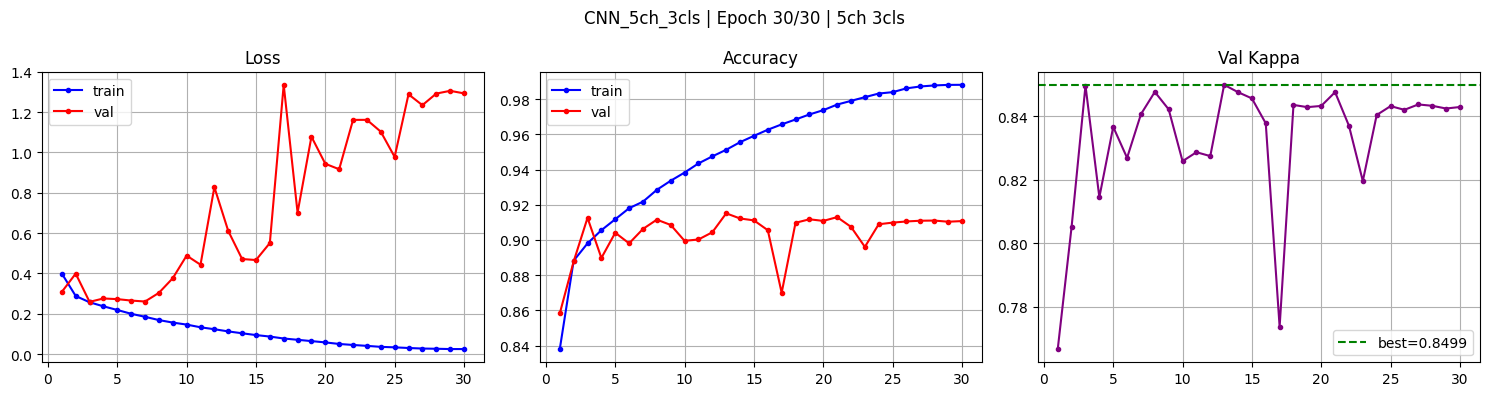
\includegraphics[width=\textwidth]{images/resultats/curves_CNN_5ch_3cls.png}
\caption[Courbes d'apprentissage du modèle convolutif]%
        {Évolution de la perte, de l'exactitude et du $\kappa$ de validation au cours
         des trente époques d'entraînement du modèle convolutif à cinq dérivations et
         trois classes.}
\label{fig:courbes}
\end{figure}

\subsubsection{Résultats}

\paragraph{Les douze modèles}

\begin{table}[H]
\centering

\small
\begin{tabular}{@{}llcccc@{}}
\toprule
\textbf{Configuration} & \textbf{Architecture} & \textbf{Exactitude} &
\textbf{$\kappa$} & \textbf{F1 macro} & \textbf{F1 pondéré} \\
\midrule
\multirow{3}{*}{5 dérivations, 3 classes}
 & Convolutif   & \textbf{\SI{91,66}{\percent}} & \textbf{0,853} & 0,89 & 0,92 \\
 & Récurrent    & \SI{90,86}{\percent} & 0,843 & 0,89 & 0,91 \\
 & Attentionnel & \SI{90,14}{\percent} & 0,826 & 0,87 & 0,90 \\
\midrule
\multirow{3}{*}{2 dérivations, 3 classes}
 & Convolutif   & \SI{89,10}{\percent} & 0,810 & 0,86 & 0,89 \\
 & Récurrent    & \SI{87,58}{\percent} & 0,790 & 0,84 & 0,88 \\
 & Attentionnel & \SI{86,92}{\percent} & 0,771 & 0,83 & 0,87 \\
\midrule
\multirow{3}{*}{5 dérivations, 5 classes}
 & Convolutif   & \SI{82,78}{\percent} & 0,761 & 0,72 & 0,83 \\
 & Récurrent    & \SI{78,60}{\percent} & 0,713 & 0,71 & 0,80 \\
 & Attentionnel & \SI{81,55}{\percent} & 0,742 & 0,70 & 0,81 \\
\midrule
\multirow{3}{*}{2 dérivations, 5 classes}
 & Convolutif   & \SI{79,90}{\percent} & 0,723 & 0,69 & 0,80 \\
 & Récurrent    & \SI{76,01}{\percent} & 0,679 & 0,68 & 0,78 \\
 & Attentionnel & \SI{77,15}{\percent} & 0,686 & 0,66 & 0,77 \\
\bottomrule
\end{tabular}
\caption{Performances des douze modèles de base sur le jeu de test}
\label{tab:12modeles}
\end{table}

Trois enseignements se dégagent.

\subparagraph{L'apport des dérivations oculaires et musculaires est net.} À granularité
constante, le passage de deux à cinq dérivations gagne entre \num{2,6} et \num{3,9}
points d'exactitude. Ce résultat était attendu : l'électro-oculogramme et
l'électromyogramme portent précisément l'information qui distingue le sommeil paradoxal.

\subparagraph{Le passage à cinq stades coûte cher.} La même architecture perd entre
\num{8,6} et \num{12,3} points en passant de trois à cinq classes.

\subparagraph{Le convolutif domine, mais de peu.} Il arrive en tête sur les quatre
configurations. L'écart avec les deux autres architectures reste toutefois inférieur à
quatre points, ce qui confirme qu'aucune famille ne domine franchement, et surtout que
leurs erreurs ne sont pas identiques.

La figure~\ref{fig:cm-3archi} rend cette dernière affirmation visible : les trois
matrices portent sur le même jeu de test, mais leurs erreurs ne se situent pas aux mêmes
endroits. C'est cette complémentarité que l'empilement, au sprint suivant, exploitera.

\begin{figure}[H]
\centering
\begin{subfigure}[t]{0.325\textwidth}
  \centering
  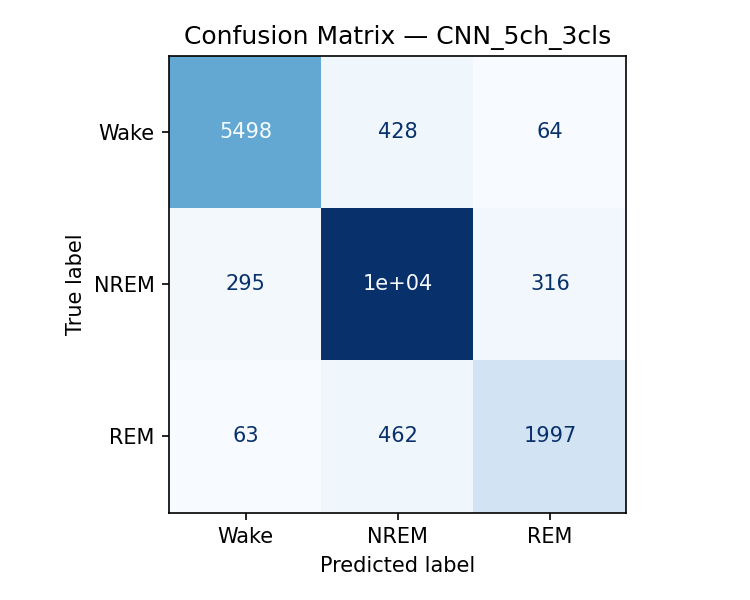
\includegraphics[width=\linewidth]{images/resultats/cm_CNN_5ch_3cls.png}
  \caption{Convolutif}
\end{subfigure}
\hfill
\begin{subfigure}[t]{0.325\textwidth}
  \centering
  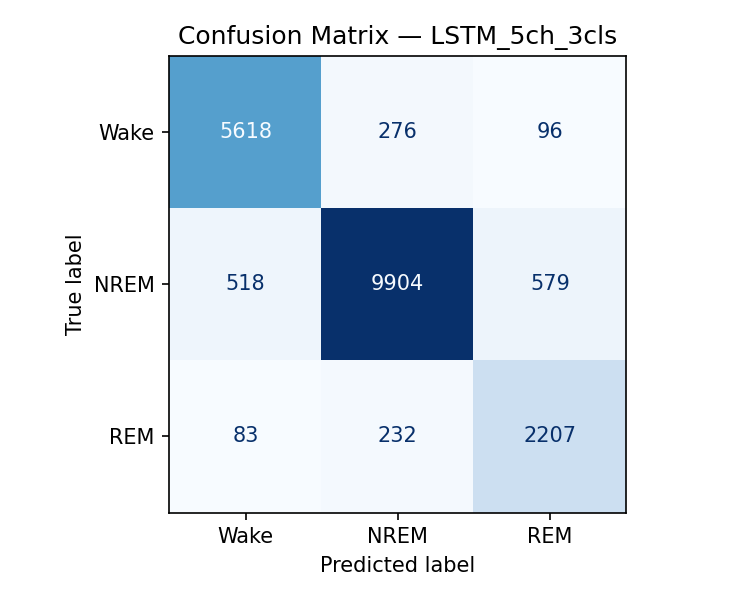
\includegraphics[width=\linewidth]{images/resultats/cm_LSTM_5ch_3cls.png}
  \caption{Récurrent}
\end{subfigure}
\hfill
\begin{subfigure}[t]{0.325\textwidth}
  \centering
  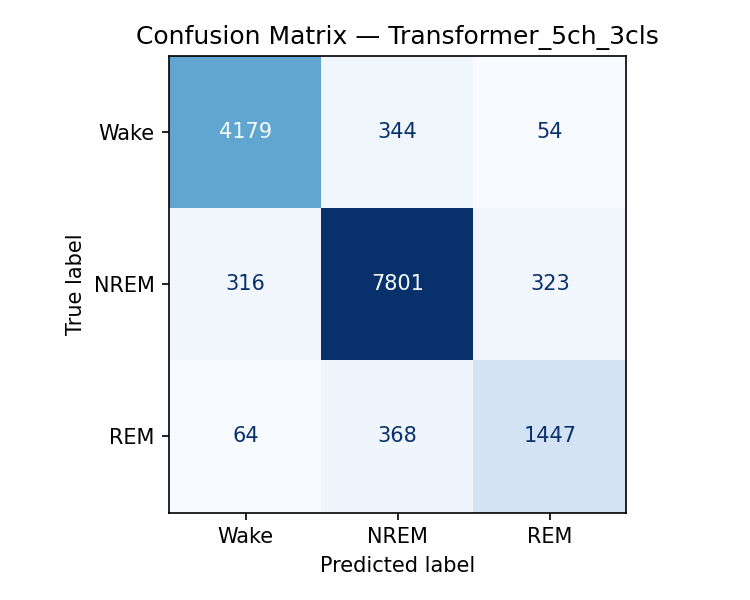
\includegraphics[width=\linewidth]{images/resultats/cm_Transformer_5ch_3cls.png}
  \caption{Attentionnel}
\end{subfigure}
\caption[Matrices de confusion des trois architectures]%
        {Matrices de confusion des trois architectures, configuration à cinq
         dérivations et trois classes. Effectifs bruts.}
\label{fig:cm-3archi}
\end{figure}

\paragraph{Le problème du stade N1}

\begin{table}[H]
\centering

\small
\begin{tabular}{@{}llcccc@{}}
\toprule
& \textbf{Classe} & \textbf{Précision} & \textbf{Rappel} & \textbf{F1} &
\textbf{Effectif} \\
\midrule
\multirow{3}{*}{\rotatebox{90}{\scriptsize 3 classes}}
 & Éveil & 0,94 & 0,92 & 0,93 & \num{5990} \\
 & NREM  & 0,92 & 0,94 & 0,93 & \num{11001} \\
 & REM   & 0,84 & 0,79 & 0,82 & \num{2522} \\
\midrule
\multirow{5}{*}{\rotatebox{90}{\scriptsize 5 classes}}
 & Éveil & 0,92 & 0,92 & 0,92 & \num{5990} \\
 & N1    & \textcolor{hypnored}{\textbf{0,29}} &
           \textcolor{hypnored}{\textbf{0,24}} &
           \textcolor{hypnored}{\textbf{0,26}} & \num{638} \\
 & N2    & 0,86 & 0,78 & 0,82 & \num{7832} \\
 & N3    & 0,70 & 0,88 & 0,78 & \num{2531} \\
 & REM   & 0,80 & 0,84 & 0,82 & \num{2522} \\
\bottomrule
\end{tabular}
\caption{Performances par classe --- configuration à cinq dérivations}
\label{tab:parclasse}
\end{table}

Le stade N1 est la seule classe véritablement échouée, avec un F1 de \num{0,26} pour le
modèle convolutif. Les autres architectures ne font pas mieux (le récurrent atteint
\num{0,30} et l'attentionnel \num{0,21}), mais elles échouent différemment. Le récurrent affiche un rappel de \num{0,59} pour une
précision de \num{0,20} : il sur-prédit massivement le N1. Le convolutif fait l'inverse,
avec un rappel de \num{0,24} pour une précision de \num{0,29}.

La figure~\ref{fig:cm-5cls} montre où partent les époques de N1 mal classées.

\begin{figure}[H]
\centering
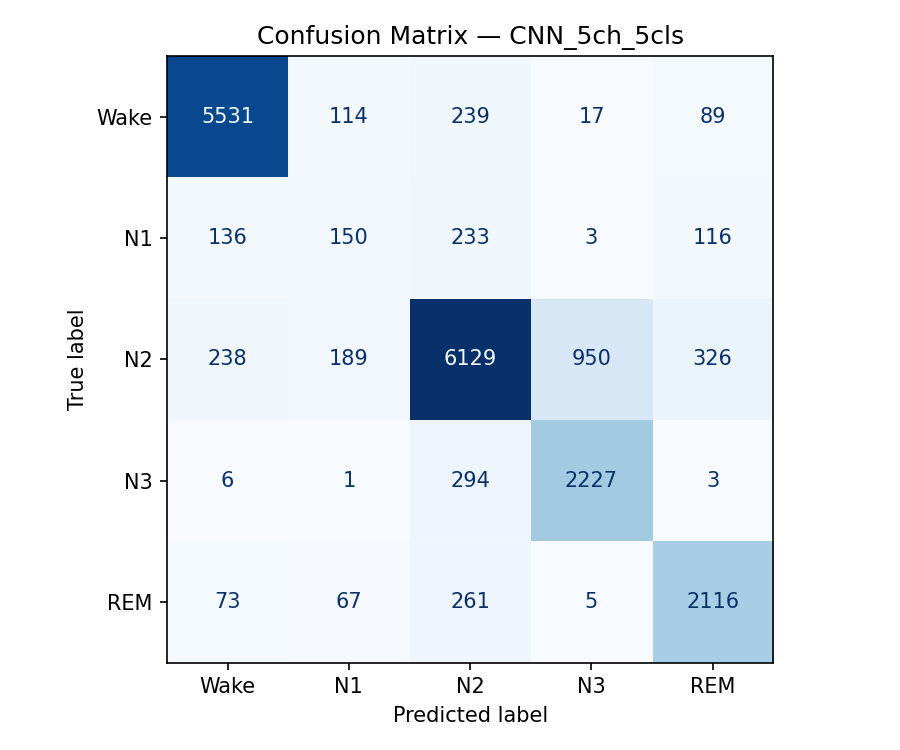
\includegraphics[width=0.72\textwidth]{images/resultats/cm_CNN_5ch_5cls.png}
\caption[Matrice de confusion à cinq classes]%
        {Matrice de confusion du modèle convolutif à cinq dérivations et cinq
         classes. Effectifs bruts sur les \num{19513} époques de test.}
\label{fig:cm-5cls}
\end{figure}

Sur les \num{638} époques réellement en N1, \num{150} seulement sont reconnues. Les
autres se dispersent : \num{233} sont versées en N2, \num{136} en éveil et \num{116} en
sommeil paradoxal. Cette dispersion n'est pas un défaut d'apprentissage mais le reflet de
la définition même du stade, un état de transition sans marqueur graphique propre. Le
modèle le classe dans les états qui l'encadrent, ce que fait aussi un scoreur humain
hésitant.

On observe par ailleurs une seconde confusion, de nature différente : \num{950} époques
de N2 sont classées en N3. Celle-ci relève d'un seuil et non d'une ambiguïté : le
référentiel AASM fixe le passage en N3 à \SI{20}{\percent} d'ondes lentes dans la
fenêtre, et une époque à \SI{19}{\percent} est presque indiscernable d'une époque à
\SI{21}{\percent}.

\subsection{Revue du sprint}

Ce sprint a produit douze modèles de classification couvrant trois architectures, deux
montages et deux granularités. La meilleure variante, le réseau convolutif à cinq
dérivations et trois classes, atteint \SI{91,66}{\percent} d'exactitude pour un
$\kappa$ de \num{0,853}, au voisinage de l'accord inter-expert rapporté dans la
littérature.

Le sprint a surtout imposé un arbitrage explicite : restreindre la cohorte pour maintenir
le corpus en mémoire vive, et préserver ainsi la qualité de convergence plutôt que le
volume de données. Cet arbitrage sera rediscuté dans la synthèse méthodologique du sprint
suivant (section~\ref{sec:synthese}).

Enfin, l'analyse par classe a révélé que les trois architectures échouent différemment sur
le stade N1. C'est la condition d'efficacité de la combinaison de modèles, que
le sprint~3 met en œuvre en ouverture de la release suivante.

% ---------------------------------------------------------------------------
\section{Revue de la release 1}
\label{sec:revue-release1}
% ---------------------------------------------------------------------------

\subsection{Incrément livré}

La release a livré l'intégralité de son backlog, soit 76 points en deux sprints. Le
tableau~\ref{tab:revue-r1} confronte l'incrément attendu à celui qui a été démontré à
l'encadrement lors de la revue.

\begin{table}[H]
\centering\small
\renewcommand{\arraystretch}{1.2}
\begin{tabular}{@{}L{3.6cm}|L{9.4cm}|c@{}}
\hline
\ligneentete \entete{Élément attendu} & \entete{Réalisation} & \entete{État} \\
\hline
Chaîne de préparation & Six étapes, du décodage du fichier EDF à la sérialisation en
tenseurs ; script relançable & \checkmark \\
\hline
Corpus d'apprentissage & \num{195130} époques étiquetées issues de 196 enregistrements
SHHS1, découpées en \num{80} / \num{10} / \num{10} & \checkmark \\
\hline
Modèles de base & Douze modèles (trois architectures, deux montages, deux
granularités) évalués sur un protocole identique & \checkmark \\
\hline
Niveau de performance & Meilleure variante, convolutive à cinq dérivations et trois
classes : \SI{91,66}{\percent} d'exactitude pour un $\kappa$ de \num{0,853} & \checkmark \\
\hline
\end{tabular}
\caption{Revue de la release 1 : incrément attendu et incrément livré}
\label{tab:revue-r1}
\end{table}

\subsection{Rétrospective}

La rétrospective de la release a dégagé trois enseignements, qui ont orienté la
planification de la suivante.

\subparagraph{Occuper les délais externes plutôt que les subir.} Le recours au jeu public
Sleep-EDF pendant l'instruction de la demande d'accès a permis de disposer d'une chaîne
éprouvée dès l'arrivée des données. Attendre l'autorisation aurait immobilisé le premier
sprint tout entier.

\subparagraph{Assumer la contrainte matérielle.} La résidence intégrale du corpus en
mémoire vive a imposé de restreindre la cohorte à 196 sujets. L'arbitrage a préservé la
qualité de convergence des douze modèles, mais il borne la portée des résultats ; il est
rediscuté dans la synthèse méthodologique de la release suivante
(section~\ref{sec:synthese}).

\subparagraph{Tirer parti de la complémentarité des erreurs.} Les trois architectures
échouent différemment, en particulier sur le stade N1. Ce constat a placé la combinaison
des modèles en tête du backlog de la release suivante.

\sectionsansnum{Conclusion}

Cette première release a livré le moteur de classification de \hypnoria{} : une chaîne de
préparation éprouvée, un corpus de \num{195130} époques étiquetées et douze modèles de base,
dont le meilleur atteint un $\kappa$ de \num{0,853}, au voisinage de l'accord inter-expert
rapporté dans la littérature.

Cet incrément reste toutefois invisible pour le praticien, et il se limite à la description
du sommeil. La release suivante le prolonge vers le diagnostic, en combinant les modèles
et en prédisant de manière explicable la sévérité du syndrome d'apnées, puis le rend
accessible depuis un poste de travail sécurisé.
    % Release 1 : sprints 1 et 2
\chapter{Release 2 : Diagnostic expliqué et poste de travail}
\label{chap:release2}

\sectionsansnum{Introduction}

Ce chapitre présente la deuxième release, menée de la semaine 9 à la semaine 16. Là où la
première a produit un moteur de classification, celle-ci livre la première version de
\hypnoria{} utilisable par un médecin : à partir d'un enregistrement brut, le praticien
obtient l'hypnogramme, les métriques du sommeil et une prédiction de la sévérité du syndrome
d'apnées accompagnée de ses facteurs explicatifs. Nous présentons l'objectif et le backlog
de la release, détaillons ses deux sprints, puis en dressons la revue.

% ---------------------------------------------------------------------------
\section{Présentation de la release}
\label{sec:release2}
% ---------------------------------------------------------------------------

\subsection{Objectif de la release}

La deuxième release vise à livrer un produit minimum viable : le plus petit
incrément qui apporte au praticien la valeur centrale du projet, à savoir un diagnostic
expliqué. Elle réunit deux sprints de natures différentes. Le sprint~3 prolonge le travail
de modélisation : il combine les modèles de base, construit le modèle de sévérité et son
mécanisme d'explication. Le sprint~4 expose l'ensemble à travers une interface applicative
sécurisée et un poste de travail guidé.

Pris isolément, aucun de ces deux sprints ne constitue une version livrable : des modèles
sans interface ne servent pas le praticien, et une interface sans modèle de sévérité ne
délivre pas le diagnostic attendu. C'est leur réunion qui forme l'incrément de la release.

\subsection{Backlog de la release}

La release regroupe vingt récits issus de cinq épics (authentification, classification,
sévérité du SAOS, visualisation et export), pour 122 points de complexité
(tableau~\ref{tab:rel2}).

\begin{table}[H]
\centering\small
\renewcommand{\arraystretch}{1.2}
\begin{tabular}{@{}L{1.4cm}|L{3.0cm}|L{5.4cm}|L{2.7cm}|c@{}}
\hline
\ligneentete \entete{Sprint} & \entete{Période} & \entete{Objectif du sprint} &
\entete{Récits} & \entete{Pts} \\
\hline
Sprint 3 & 23 mars -- 19 avr. &
Faire coopérer les architectures, puis prédire de manière explicable la sévérité du SAOS &
US-13 à 16 & 42 \\
\hline
Sprint 4 & 20 avr. -- 17 mai &
Rendre les modèles consommables et offrir au praticien un parcours d'analyse guidé &
US-09 à 12, 17 à 23, 26 à 29, 40 & 80 \\
\hline
\multicolumn{3}{@{}r|}{\textbf{Total de la release}} & \textbf{20 récits} & \textbf{122} \\
\hline
\end{tabular}
\caption{Backlog de la release 2}
\label{tab:rel2}
\end{table}

\noindent
L'incrément attendu en fin de release est un parcours complet, de l'authentification du
praticien jusqu'au rapport de sévérité expliqué, reposant sur quatre ensembles de
classification et sur un modèle de sévérité.

% ---------------------------------------------------------------------------
\section{Sprint 3 : Ensembles et prédiction de la sévérité}
\label{sec:sprint3}
% ---------------------------------------------------------------------------

Premier sprint de la release, le sprint~3 articule deux travaux complémentaires. Le premier
fait coopérer les modèles de la release précédente par un mécanisme d'empilement. Le second
franchit un pas supplémentaire : passer de la description du sommeil au \emph{diagnostic},
en prédisant la sévérité d'un syndrome d'apnées à partir de l'hypnogramme produit, et en
expliquant chaque prédiction. Le sprint se conclut sur une synthèse méthodologique qui
discute les limites de l'ensemble des résultats obtenus depuis le sprint~1.

\subsection{Objectif du sprint}

Le sprint poursuivait trois objectifs.

Le premier était de tirer parti de la complémentarité des architectures mise en
évidence au sprint 2. Les trois familles échouent différemment, notamment sur le stade
N1 : c'est la condition d'efficacité d'une combinaison de modèles.

Le deuxième était d'exploiter l'hypnogramme comme marqueur indirect du syndrome
d'apnées. L'hypothèse est que les micro-éveils répétés provoqués par les obstructions
laissent une empreinte mesurable sur l'architecture du sommeil, indépendamment des
capteurs respiratoires.

Le troisième était de rendre chaque prédiction explicable, condition d'usage
clinique posée dès le chapitre~\ref{chap:presentation}.

\subsection{Sprint Backlog}

Le sprint a embarqué quatre récits pour 42 points de complexité
(tableau~\ref{tab:bl-s3}).

\begin{table}[H]
\centering\small
\renewcommand{\arraystretch}{1.15}
\begin{tabular}{@{}c|L{2.5cm}|L{4.6cm}|L{4.6cm}|c@{}}
\hline
\ligneentete \entete{ID} & \entete{Module} & \entete{R\'ecit utilisateur} & \entete{T\^aches} & \entete{Estim.} \\
\hline
\multirow{3}{*}{US-13} & \multirow{3}{=}{Ensembles} & \multirow{3}{=}{En tant que syst\`eme, je veux combiner les trois mod\`eles par un m\'eta-apprenant} & Collecter les probabilit\'es sur un jeu de validation par sujets & \multirow{3}{*}{13 pts} \\
 &  &  & Entra\^iner une r\'egression logistique \'equilibr\'ee &  \\
 &  &  & Comparer au vote moyen et au meilleur mod\`ele isol\'e &  \\
\hline
\multirow{3}{*}{US-14} & \multirow{3}{=}{Marqueurs du sommeil} & \multirow{3}{=}{En tant que syst\`eme, je veux extraire les marqueurs d'architecture du sommeil depuis l'hypnogramme} & Analyser les hypnogrammes de la seconde visite & \multirow{3}{*}{8 pts} \\
 &  &  & Calculer 25 marqueurs conformes au r\'ef\'erentiel AASM &  \\
 &  &  & Construire 8 variables d'interaction &  \\
\hline
\multirow{3}{*}{US-15} & \multirow{3}{=}{Pr\'ediction de s\'ev\'erit\'e} & \multirow{3}{=}{En tant que syst\`eme, je veux pr\'edire la s\'ev\'erit\'e du SAOS en quatre classes} & \'Ecarter les variables qui fuient la cible & \multirow{3}{*}{13 pts} \\
 &  &  & Comparer six familles de classifieurs en validation crois\'ee &  \\
 &  &  & Empiler les trois meilleurs vers un m\'eta-apprenant &  \\
\hline
\multirow{3}{*}{US-16} & \multirow{3}{=}{Explicabilit\'e} & \multirow{3}{=}{En tant que m\'edecin, je veux conna\^itre les facteurs aggravants et protecteurs de la pr\'ediction} & Calculer les attributions par valeurs de Shapley & \multirow{3}{*}{8 pts} \\
 &  &  & Trier et restituer les dix facteurs dominants &  \\
 &  &  & S\'eparer contributions positives et n\'egatives &  \\
\hline
\end{tabular}
\caption{Sprint Backlog --- Sprint 3}
\label{tab:bl-s3}
\end{table}

\subsection{Analyse}

\subsubsection{Diagramme des cas d'utilisation}

\begin{figure}[H]
\centering
\begin{tikzpicture}[
    x=1cm,y=1cm,
    uc/.style     = {ellipse, draw=hypnoblue!60, fill=hypnolight,
                     align=center, font=\scriptsize, text width=2.7cm,
                     inner sep=1.5pt, minimum height=1.0cm},
    ucp/.style    = {ellipse, draw=hypnored!70, fill=hypnored!7,
                     align=center, font=\scriptsize\bfseries, text width=2.7cm,
                     inner sep=1.5pt, minimum height=1.0cm},
    lien/.style   = {hypnogray!75, line width=0.55pt},
    rel/.style    = {-{Latex[length=2mm]}, hypnoblue!70, line width=0.5pt, dashed},
    et/.style     = {font=\tiny\itshape, text=hypnoblue!85, fill=white, inner sep=1pt},
    nomact/.style = {font=\scriptsize\bfseries, align=center, text width=2.2cm},
  ]

  \tikzset{acteur/.pic={
      \draw[hypnoblue,line width=0.8pt] (0,0) circle (0.17);
      \draw[hypnoblue,line width=0.8pt] (0,-0.17) -- (0,-0.66);
      \draw[hypnoblue,line width=0.8pt] (-0.28,-0.34) -- (0.28,-0.34);
      \draw[hypnoblue,line width=0.8pt] (0,-0.66) -- (-0.24,-1.04);
      \draw[hypnoblue,line width=0.8pt] (0,-0.66) -- (0.24,-1.04);}}

  \draw[hypnoblue!55,line width=0.9pt,rounded corners=3pt]
       (3.6,-4.6) rectangle (12.6,2.4);
  \node[font=\small\bfseries,text=hypnoblue,anchor=north west] at (3.85,2.25)
       {Module de diagnostic};

  \node[ucp] (sev) at (5.7, 0.7)  {Prédire la\\sévérité du SAOS};
  \node[uc]  (ens) at (5.7,-3.0)  {Combiner les\\modèles de base};

  \node[uc]  (mar) at (10.2, 1.2) {Extraire les marqueurs\\d'architecture};
  \node[uc]  (imp) at (10.2,-0.3) {Imputer les valeurs\\manquantes};
  \node[uc]  (pre) at (10.2,-1.8) {Classer en quatre\\niveaux de sévérité};
  \node[uc]  (exp) at (10.2,-3.3) {Attribuer les\\contributions};

  \pic at (1.5,0.4) {acteur};
  \node[nomact,anchor=north] at (1.5,-0.25) {Médecin};

  \pic at (1.5,-2.6) {acteur};
  \node[nomact,anchor=north] at (1.5,-3.25) {Moteur\\d'inférence};

  \draw[lien] (1.9,0.05) -- (sev.west);
  \draw[lien] (1.9,-2.95) -- (ens.west);

  \draw[rel] (sev) -- node[et,pos=0.62] {$\ll$include$\gg$} (mar);
  \draw[rel] (sev) -- node[et,pos=0.62] {$\ll$include$\gg$} (imp);
  \draw[rel] (sev) -- node[et,pos=0.64] {$\ll$include$\gg$} (pre);
  \draw[rel] (sev) -- node[et,pos=0.68] {$\ll$include$\gg$} (exp);

\end{tikzpicture}
\caption{Diagramme des cas d'utilisation du sprint 3 --- diagnostic et explication}
\label{fig:uc-s3}
\end{figure}

\subsubsection{Description textuelle des cas d'utilisation}

\begin{casutilisation}{Description textuelle du cas « Prédire la sévérité du SAOS »}
Titre & Prédire la sévérité du SAOS \\ \hline
Acteurs & Médecin du sommeil, moteur d'inférence \\ \hline
Description & Estimer le niveau de sévérité du syndrome d'apnées obstructives à partir
de l'architecture du sommeil et de marqueurs cliniques, et exposer les facteurs qui
déterminent cette estimation \\ \hline
Préconditions & Une séquence de stades est disponible, issue d'une analyse ou d'une
saisie manuelle \\ \hline
Scénario de base &
\begin{minipage}[t]{\linewidth}
\begin{enumerate}[leftmargin=1.1em,itemsep=1pt,topsep=3pt]
  \item Le système extrait les marqueurs d'architecture depuis l'hypnogramme.
  \item Le médecin complète les données démographiques et oxymétriques.
  \item Il déclenche l'évaluation du risque.
  \item Le système construit le vecteur de variables et comble les valeurs absentes.
  \item Le moteur produit la classe de sévérité et ses probabilités.
  \item Le système calcule les contributions de chaque variable.
  \item Le système affiche la sévérité, les facteurs aggravants et protecteurs, et
        l'interprétation clinique.
\end{enumerate}
\end{minipage} \\ \hline
Scénario alternatif &
\begin{minipage}[t]{\linewidth}
\begin{itemize}[leftmargin=1.1em,itemsep=1pt,topsep=3pt]
  \item \textbf{2a} --- Le médecin importe un rapport externe : le système en extrait les
        valeurs et préremplit le formulaire.
  \item \textbf{4a} --- Des variables cliniques manquent : le système applique la médiane
        de la population d'apprentissage et le signale.
  \item \textbf{5a} --- Les modèles ne sont pas chargés : l'opération est refusée avec un
        message explicite.
\end{itemize}
\end{minipage}
\end{casutilisation}

\subsection{Conception}

\subsubsection{Diagramme de séquence objet}

\begin{figure}[H]
\centering
\resizebox{0.93\textwidth}{!}{%
\begin{sequencediagram}
  \newthread[hypnolight]{u}{\scriptsize Praticien}
  \newinst[2.2]{f}{\scriptsize Client web}
  \newinst[2.2]{a}{\scriptsize Interface applicative}
  \newinst[2.2]{m}{\scriptsize Moteur d'inférence}

  \begin{call}{u}{\scriptsize saisit les données cliniques}{f}{}
  \end{call}
  \begin{call}{f}{\scriptsize demande d'évaluation}{a}{\scriptsize sévérité et facteurs}
    \begin{call}{a}{\scriptsize extraction des marqueurs}{a}{}
    \end{call}
    \begin{call}{a}{\scriptsize imputation et alignement}{a}{}
    \end{call}
    \begin{call}{a}{\scriptsize prédiction}{m}{\scriptsize classe et probabilités}
    \end{call}
    \begin{call}{a}{\scriptsize attribution des contributions}{m}{\scriptsize facteurs}
    \end{call}
  \end{call}
  \begin{call}{f}{\scriptsize affiche le rapport expliqué}{u}{}
  \end{call}
\end{sequencediagram}}
\caption[Séquence de prédiction de la sévérité]%
        {Prédiction de la sévérité et production des facteurs explicatifs.}
\label{fig:seq-osa}
\end{figure}

\subsection{Réalisation}

\subsubsection{Combinaison des modèles par empilement}

\paragraph{Principe}

L'\emph{empilement}, introduit par Wolpert~\cite{wolpert1992}, consiste à entraîner un
second modèle, le \emph{méta-apprenant}, à combiner les sorties de plusieurs
modèles de base. Contrairement au vote majoritaire, qui accorde le même poids à tous, le
méta-apprenant \emph{apprend} à qui faire confiance et dans quelles circonstances
(figure~\ref{fig:stacking-principe}).

\begin{figure}[H]
\centering
\begin{tikzpicture}[
    x=1cm,y=1cm,
    bloc/.style   = {rectangle,rounded corners=2pt,draw=hypnoblue!60,fill=hypnolight,
                     align=center,font=\small,minimum height=1.0cm,text width=2.5cm},
    meta/.style   = {rectangle,rounded corners=2pt,draw=hypnored!75,fill=hypnored!8,
                     align=center,font=\small,minimum height=1.0cm,text width=2.8cm},
    ent/.style    = {rectangle,rounded corners=2pt,draw=hypnogray!60,fill=white,
                     align=center,font=\small,minimum height=1.0cm,text width=2.0cm},
    fl/.style     = {-{Latex[length=2.2mm]},hypnoblue!75,line width=0.8pt},
    lab/.style    = {font=\scriptsize\itshape,text=hypnogray},
  ]

  \node[ent]  (x)   at (0,0)      {Époque\\$(5 \times 3000)$};

  \node[bloc] (cnn) at (3.6,2.0)  {CNN};
  \node[bloc] (lstm)at (3.6,0)    {BiLSTM};
  \node[bloc] (tr)  at (3.6,-2.0) {Transformer};

  \node[ent]  (cat) at (7.3,0)    {Concaténation\\$(M \times C)$};
  \node[meta] (ml)  at (10.9,0)   {Méta-apprenant\\\scriptsize régression logistique};
  \node[ent]  (out) at (14.1,0)   {Stade\\prédit};

  \draw[fl] (x) -- (cnn);
  \draw[fl] (x) -- (lstm);
  \draw[fl] (x) -- (tr);

  \draw[fl] (cnn) -- node[lab,above,pos=0.5,yshift=1pt] {$p_1$} (cat);
  \draw[fl] (lstm)-- node[lab,above,pos=0.5,yshift=1pt] {$p_2$} (cat);
  \draw[fl] (tr)  -- node[lab,above,pos=0.5,yshift=1pt] {$p_3$} (cat);

  \draw[fl] (cat) -- (ml);
  \draw[fl] (ml)  -- (out);

  % Bandeaux de niveau
  \node[lab,anchor=north] at (3.6,-3.05) {Niveau 0 --- modèles de base};
  \node[lab,anchor=north] at (10.9,-3.05) {Niveau 1 --- méta-apprenant};
  \draw[hypnogray!45,dashed,line width=0.5pt] (5.6,3.1) -- (5.6,-3.0);

\end{tikzpicture}
\vspace{0.4cm}
\caption[Principe de l'empilement de modèles]%
        {Principe de l'empilement : trois modèles hétérogènes produisent des vecteurs
         de probabilités, qu'un méta-apprenant apprend à combiner.}
\label{fig:stacking-principe}
\end{figure}

Chaque modèle produit un vecteur de probabilités sur les $K$ classes ; les trois vecteurs
sont concaténés en $3K$ méta-caractéristiques qui alimentent une régression logistique
équilibrée. Le choix d'un modèle linéaire pour le second niveau est délibéré :
le méta-apprenant dispose de peu de variables et doit avant tout produire
des probabilités calibrées, ce qu'un modèle simple fait mieux qu'un réseau
supplémentaire~\cite{ting1999}.

Le point critique est le jeu sur lequel le méta-apprenant est entraîné. L'entraîner sur
les sorties produites par les modèles de base \emph{sur leurs propres données
d'entraînement} fausserait l'apprentissage : ces sorties sont anormalement bonnes, et
le méta-apprenant apprendrait une confiance injustifiée. Les probabilités ont donc été
collectées sur un jeu de validation constitué par découpage au niveau des sujets.

\paragraph{Résultats}

Quatre ensembles ont été construits, un par configuration.

\begin{table}[H]
\centering

\small
\begin{tabular}{@{}lcccccc@{}}
\toprule
\textbf{Configuration} & \textbf{Conv.} & \textbf{Réc.} & \textbf{Att.} &
\textbf{Vote moyen} & \textbf{Empilement} & \textbf{Gain} \\
\midrule
5 dérivations, 3 classes & 0,932 & 0,875 & 0,944 & \textbf{0,950} & 0,947 &
\textcolor{hypnored}{$-$0,003} \\
2 dérivations, 3 classes & 0,863 & 0,821 & 0,918 & 0,917 & \textbf{0,924} & $+$0,006 \\
5 dérivations, 5 classes & 0,875 & 0,754 & 0,887 & 0,894 & \textbf{0,899} & $+$0,005 \\
2 dérivations, 5 classes & 0,819 & 0,695 & 0,815 & 0,834 & \textbf{0,839} & $+$0,005 \\
\bottomrule
\end{tabular}
\vspace{2pt}
\raggedright\footnotesize
Valeurs de $\kappa$ de Cohen sur le jeu de test par sujets. Le gain est mesuré par
rapport au vote moyen.
\caption{Ensembles par empilement, comparés aux modèles de base et au vote moyen}
\label{tab:ensembles}
\end{table}

Ces résultats appellent une lecture nuancée. L'empilement dépasse le meilleur modèle
isolé sur les quatre configurations, ce qui valide le principe. Mais il ne dépasse le
vote moyen que sur trois configurations sur quatre : sur la variante à cinq dérivations et trois
classes, la moyenne arithmétique des probabilités fait légèrement mieux que le
méta-apprenant.

L'explication tient à la taille du jeu d'apprentissage du second niveau. Le
méta-apprenant est entraîné sur une vingtaine de milliers d'exemples décrits par neuf
variables seulement. Lorsque les trois modèles de base sont déjà très concordants,
ce qui est le cas dans la configuration la plus favorable, il ne reste presque rien à
apprendre, et la pondération estimée n'apporte pas davantage qu'une moyenne uniforme.

Rapporter seulement le gain sur le meilleur modèle isolé aurait donné de l'empilement
une image trop favorable. La comparaison au vote moyen, souvent
omise dans la littérature, montre que son apport est réel mais modeste, et qu'il dépend
du degré de désaccord entre les modèles combinés.

\begin{figure}[H]
\centering
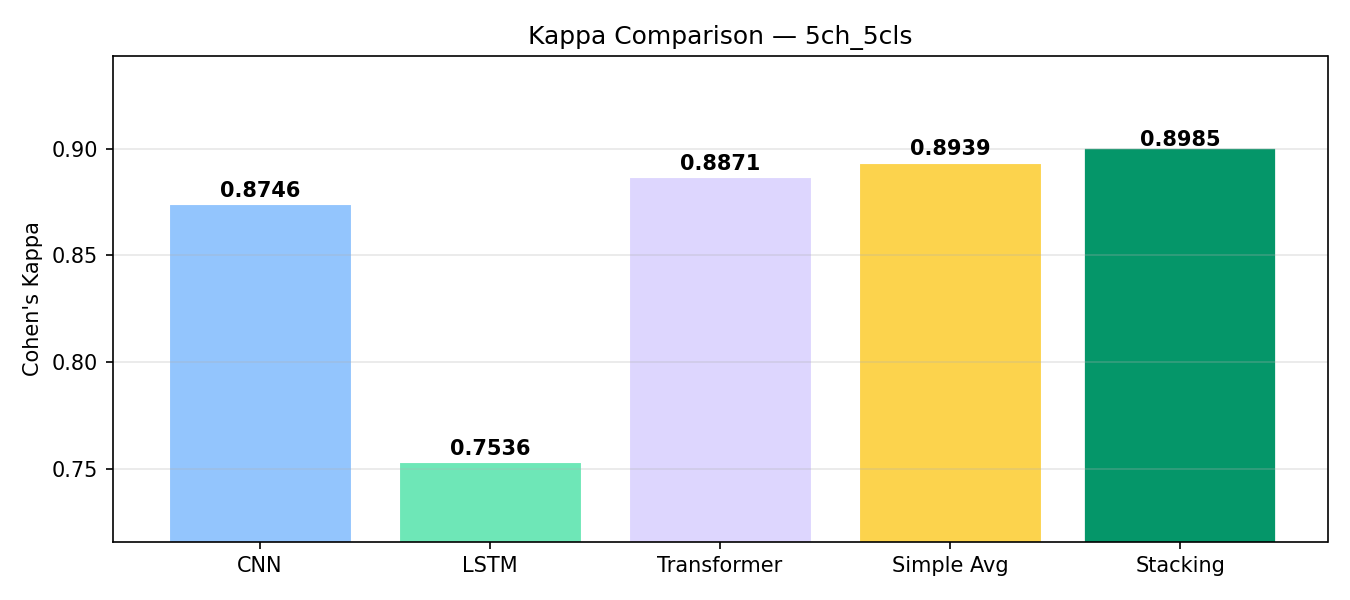
\includegraphics[width=0.92\textwidth]{images/resultats/kappa_comparison_5ch_5cls.png}
\caption[Comparaison des $\kappa$ pour l'ensemble à cinq classes]%
        {Comparaison des $\kappa$ obtenus par les modèles de base, le vote moyen et
         l'empilement, pour la configuration à cinq dérivations et cinq classes.}
\label{fig:kappa-comp}
\end{figure}

\begin{figure}[H]
\centering
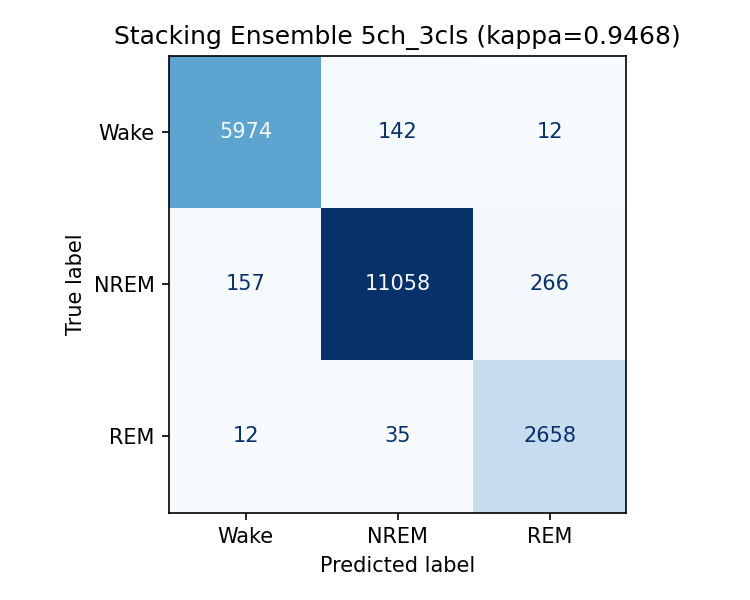
\includegraphics[width=0.62\textwidth]{images/resultats/cm_stacking_5ch_3cls.png}
\caption[Matrice de confusion de l'ensemble]%
        {Matrice de confusion de l'ensemble à cinq dérivations et trois classes, sur
         les \num{20314} époques du jeu de test par sujets.}
\label{fig:cm-stack}
\end{figure}

\subsubsection{Prédiction de la sévérité du syndrome d'apnées}

\paragraph{Positionnement}

Le dépistage du syndrome d'apnées repose classiquement sur des questionnaires cliniques
ou sur l'analyse de signaux respiratoires. Le tableau~\ref{tab:etat-art-osa} situe notre
approche parmi ces familles.

\begin{table}[H]
\centering

\small
\begin{tabular}{@{}L{3.6cm}L{3.8cm}L{3.4cm}L{2.6cm}@{}}
\toprule
\textbf{Approche} & \textbf{Entrées} & \textbf{Atouts} & \textbf{Limites} \\
\midrule
Questionnaires\newline (Berlin, STOP-BANG) & Anamnèse, anthropométrie &
Immédiat, sans matériel & Spécificité faible, pas de sévérité \\
\addlinespace[3pt]
Oxymétrie nocturne & Saturation en oxygène & Matériel léger, bon dépistage &
Sévérité imprécise \\
\addlinespace[3pt]
Signaux respiratoires\newline et cardiaques & Flux nasal, sangles, ECG &
Performances élevées & Exige les capteurs respiratoires \\
\addlinespace[3pt]
\textbf{Architecture du sommeil}\newline \emph{(voie retenue)} & Hypnogramme, oxymétrie
sommaire, index d'éveil & Réutilise l'étage de staging ; marqueurs cliniquement
lisibles & Marqueur indirect \\
\bottomrule
\end{tabular}
\caption{Approches d'évaluation du risque de SAOS}
\label{tab:etat-art-osa}
\end{table}

\paragraph{Construction de la matrice de variables}

Les marqueurs d'architecture ont été extraits de \num{2647} hypnogrammes de la seconde
visite de la cohorte, puis complétés des variables cliniques et de variables
d'interaction, pour un total de 53 variables. Le jeu a été partagé en
\SI{80}{\percent} d'apprentissage et \SI{20}{\percent} de test, soit \num{530} sujets de
test, avec stratification sur la classe de sévérité.

La figure~\ref{fig:pipeline-osa} décrit l'enchaînement complet.

\begin{figure}[H]
\centering
\begin{tikzpicture}[
    x=1cm,y=1cm,
    et/.style   = {rectangle,rounded corners=2pt,draw=hypnoblue!60,fill=hypnolight,
                   align=center,font=\tiny,minimum height=1.15cm,text width=2.3cm},
    etf/.style  = {rectangle,rounded corners=2pt,draw=hypnored!65,fill=hypnored!7,
                   align=center,font=\tiny,minimum height=1.15cm,text width=2.3cm},
    io/.style   = {rectangle,rounded corners=2pt,draw=hypnogray!60,fill=white,
                   align=center,font=\tiny,minimum height=1.15cm,text width=2.1cm},
    fl/.style   = {-{Latex[length=1.8mm]},hypnoblue!75,line width=0.7pt},
    tag/.style  = {font=\tiny\itshape,text=hypnogray,align=center},
  ]

  \node[io] (hyp) at (0,0.8)   {Hypnogramme};
  \node[io] (cli) at (0,-0.9)  {Données\\cliniques};

  \node[et] (mrq) at (3.1,0.8)  {25 marqueurs\\d'architecture};
  \node[et] (fus) at (6.2,0)    {Fusion et\\8 interactions};
  \node[et] (imp) at (9.3,0)    {Imputation par\\la médiane};
  \node[etf](mod) at (12.4,0)   {Ensemble\\par empilement};

  \node[etf](shp) at (12.4,-2.3) {Attribution des\\contributions};
  \node[io] (res) at (8.6,-2.3)  {Classe, probabilités\\et facteurs};

  \draw[fl] (hyp) -- (mrq);
  \draw[fl] (mrq) -- (fus);
  \draw[fl] (cli) -| (fus);
  \draw[fl] (fus) -- (imp);
  \draw[fl] (imp) -- (mod);
  \draw[fl] (mod) -- (shp);
  \draw[fl] (shp) -- (res);

  \node[tag,anchor=north,text width=3.6cm] at (6.2,-1.05)
       {53 variables au total};

\end{tikzpicture}
\vspace{0.3cm}
\caption[Pipeline de prédiction de la sévérité]%
        {Chaîne de prédiction de la sévérité, de l'hypnogramme à l'explication.}
\label{fig:pipeline-osa}
\end{figure}

Deux précautions méthodologiques ont été prises. Les index de perturbation
respiratoire ont été exclus des variables d'entrée : ils mesurent directement les
événements dont on cherche à prédire la sévérité, et les conserver aurait produit un
modèle excellent mais dépourvu de valeur pratique. Par ailleurs, les modèles sensibles à
l'échelle ont été encapsulés avec leur normaliseur dans un pipeline, de sorte que
celui-ci soit ajusté sur chaque pli d'entraînement seulement et jamais sur le pli
d'évaluation.

La figure~\ref{fig:distrib-osa} montre comment quelques marqueurs se comportent selon la
classe de sévérité. On y lit à la fois la validité de l'hypothèse de départ
(l'efficacité du sommeil décroît et l'index de fragmentation croît avec la sévérité) et
la difficulté de la tâche : les distributions des classes normale et légère se recouvrent
presque entièrement.

\begin{figure}[H]
\centering
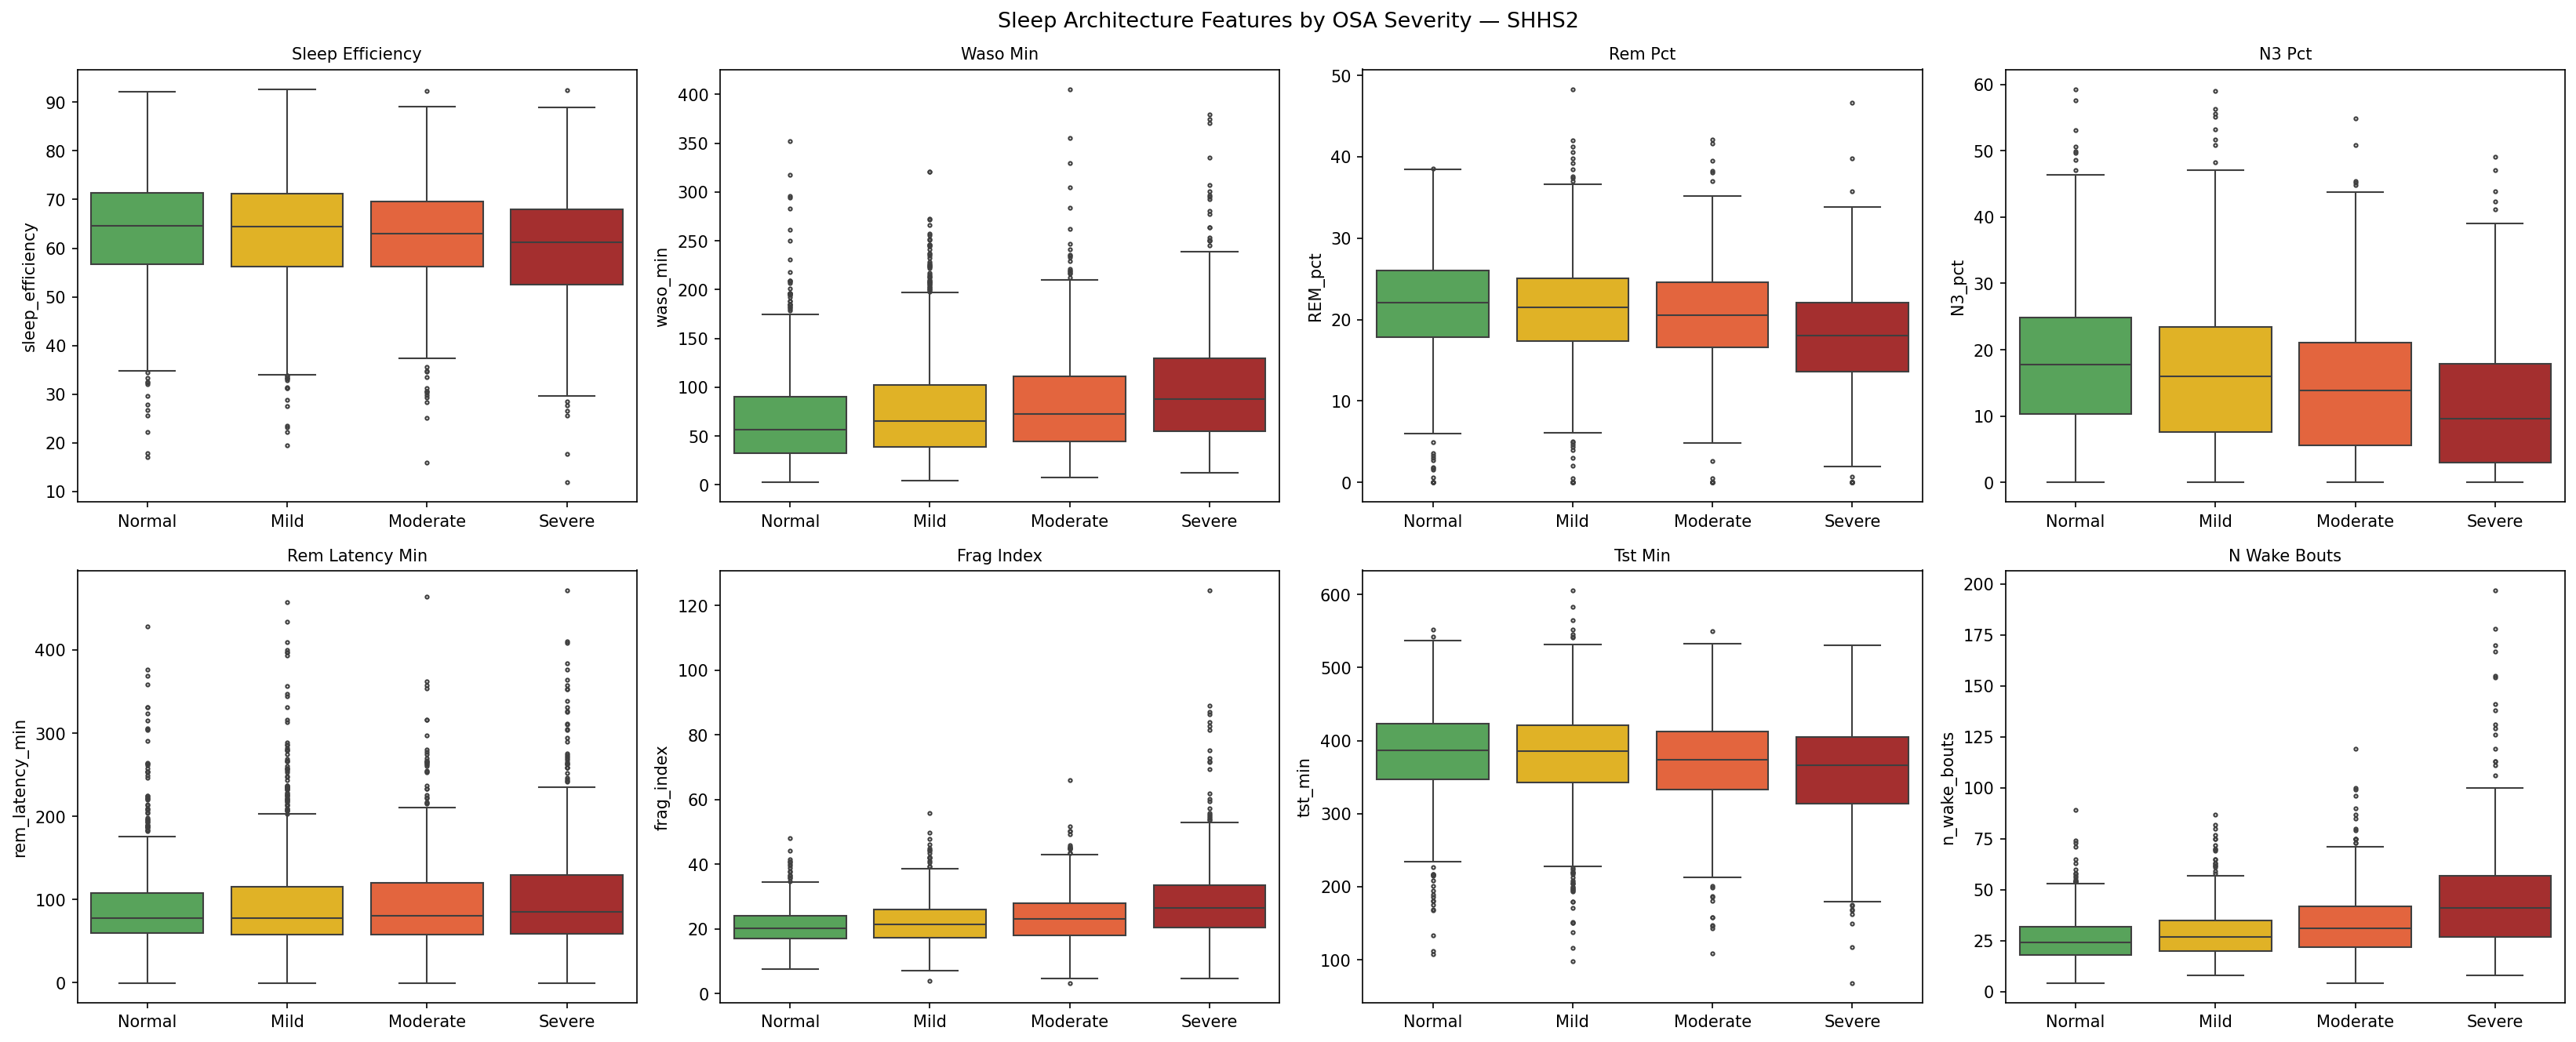
\includegraphics[width=\textwidth]{images/resultats/feature_distributions.png}
\caption[Distribution des marqueurs selon la sévérité]%
        {Distribution de huit marqueurs d'architecture du sommeil selon la classe de
         sévérité, sur la cohorte SHHS2.}
\label{fig:distrib-osa}
\end{figure}

\paragraph{Comparaison des classifieurs}

Six familles ont été comparées en validation croisée stratifiée à cinq plis, sur le F1
macro.

\begin{figure}[H]
\centering
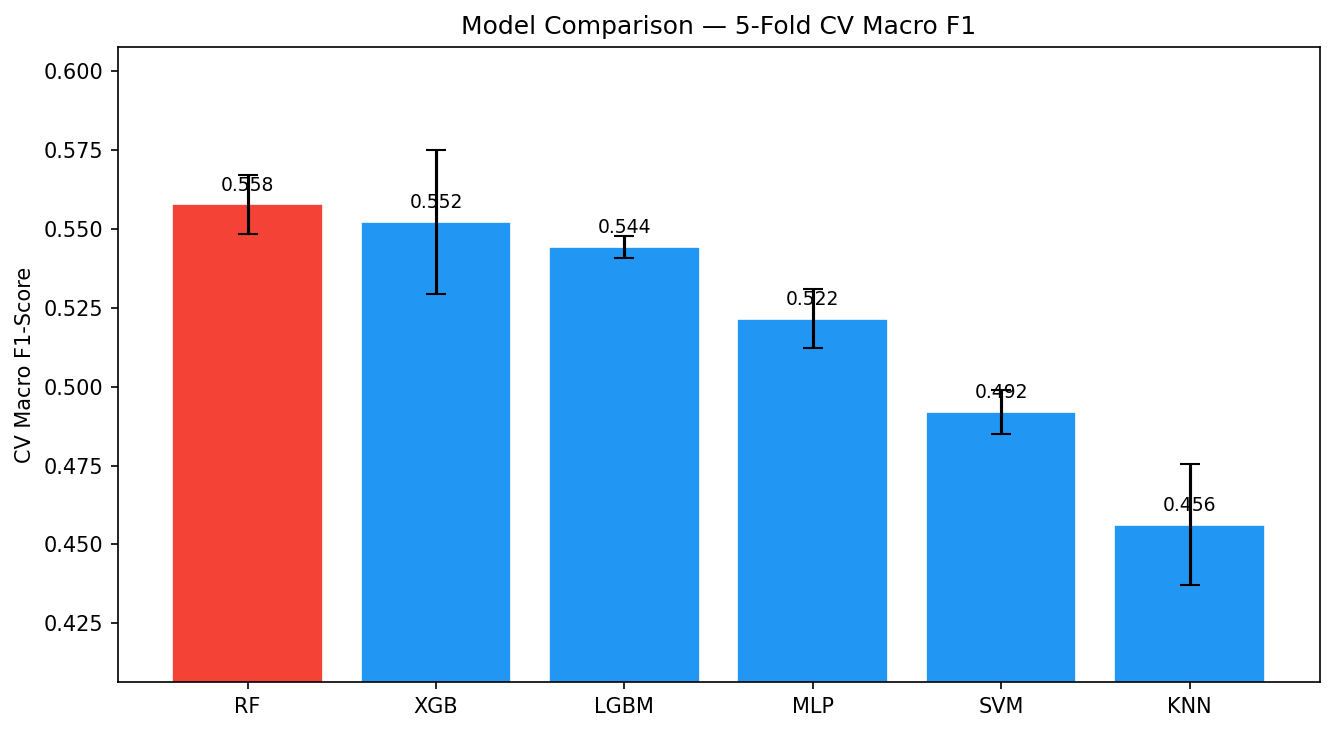
\includegraphics[width=0.88\textwidth]{images/resultats/model_comparison.png}
\caption[Comparaison des six classifieurs en validation croisée]%
        {F1 macro en validation croisée à cinq plis. La forêt aléatoire arrive en
         tête, suivie des deux implémentations de gradient boosté.}
\label{fig:comparaison-osa}
\end{figure}

La forêt aléatoire~\cite{breiman2001} obtient le meilleur score (\num{0,558}), suivie de
près par XGBoost~\cite{chen2016} (\num{0,552}) et LightGBM~\cite{ke2017} (\num{0,544}).
Le perceptron multicouche (\num{0,522}), la machine à vecteurs de support (\num{0,492}) et
les plus proches voisins (\num{0,456}) suivent. Les trois premiers ont été retenus comme
modèles de base de l'ensemble.

\paragraph{Résultats sur le jeu de test}

\begin{table}[H]
\centering

\small
\begin{tabular}{@{}lcccc@{}}
\toprule
\textbf{Modèle} & \textbf{Exactitude} & \textbf{$\kappa$} & \textbf{F1 macro} &
\textbf{Écart $\leq$ 1 classe} \\
\midrule
Forêt aléatoire & \textbf{\SI{57,0}{\percent}} & \textbf{0,409} & \textbf{0,576} &
\SI{95,5}{\percent} \\
Empilement & \SI{54,5}{\percent} & 0,389 & 0,558 & \SI{95,3}{\percent} \\
\midrule
\emph{Référence : classe majoritaire} & \SI{36,2}{\percent} & 0,000 & 0,133 & --- \\
\bottomrule
\end{tabular}
\caption{Prédiction de la sévérité --- résultats sur les 530 sujets de test}
\label{tab:osa-resultats}
\end{table}

Trois observations se dégagent de ces résultats.

\subparagraph{L'empilement n'apporte rien ici.} Contrairement au cas de la classification
des stades, il fait légèrement \emph{moins} bien que la meilleure ligne de base. Ce
résultat négatif est cohérent avec la condition de diversité : les trois modèles retenus
sont tous des ensembles d'arbres, entraînés sur les mêmes variables. Leurs erreurs se
recouvrent largement, et la combinaison n'a rien à corriger. Retenir la forêt aléatoire
seule serait ici le choix rationnel.

\subparagraph{La tâche est intrinsèquement difficile.} Une exactitude de \SI{57}{\percent}
sur quatre classes peut sembler faible, mais la référence par la classe majoritaire n'est
que de \SI{36,2}{\percent}, et le $\kappa$ de \num{0,41} correspond à un accord modéré. La
difficulté vient de la nature même des seuils : un index d'apnées de \num{4,9} et un index
de \num{5,1} classent deux patients différemment alors que rien ne les distingue
physiologiquement.

\subparagraph{L'erreur est presque toujours de faible amplitude.} Plus de \SI{95}{\percent}
des prédictions tombent dans la bonne classe ou dans une classe adjacente. C'est la
statistique cliniquement pertinente : le système se trompe rarement de plus d'un cran de
sévérité, et n'annonce quasiment jamais un patient sévère comme normal.

\begin{figure}[H]
\centering
\begin{tikzpicture}[x=1.28cm,y=1.02cm,font=\scriptsize]

  \def\CM{
    {83,38,3,2},
    {39,109,35,9},
    {4,47,54,22},
    {0,6,23,56}}

  \foreach \lab [count=\j from 0] in {Normal,Léger,Modéré,Sévère}
    \node[font=\scriptsize,anchor=base] at (\j+0.5,4.14) {\lab};
  \foreach \lab [count=\i from 0] in {Normal,Léger,Modéré,Sévère}
    \node[font=\scriptsize,anchor=east] at (-0.08,3.5-\i) {\lab};

  \foreach \row [count=\i from 0] in \CM {
    \foreach \v [count=\j from 0] in \row {
      \pgfmathsetmacro{\tot}{\i==0 ? 126 : (\i==1 ? 192 : (\i==2 ? 127 : 85))}
      \pgfmathsetmacro{\int}{100*\v/\tot}
      \pgfmathsetmacro{\diag}{\i==\j ? 1 : 0}
      \ifnum\diag=1
        \fill[hypnoblue!\int] (\j,3-\i) rectangle (\j+1,4-\i);
      \else
        \fill[hypnored!\int] (\j,3-\i) rectangle (\j+1,4-\i);
      \fi
      \draw[white,line width=0.9pt] (\j,3-\i) rectangle (\j+1,4-\i);
      \node[font=\scriptsize] at (\j+0.5,3.5-\i) {\v};
    }
  }

  \node[font=\scriptsize\itshape,anchor=north] at (2.0,-0.25) {classe prédite};
  \node[font=\scriptsize\itshape,rotate=90] at (-1.35,2.0) {classe réelle};

\end{tikzpicture}
\vspace{0.3cm}
\caption[Matrice de confusion de la prédiction de sévérité]%
        {Matrice de confusion de la forêt aléatoire sur les 530 sujets de test.
         L'intensité est proportionnée à l'effectif de chaque classe réelle.}
\label{fig:cm-osa}
\end{figure}

La lecture confirme le diagnostic. Les \num{192} sujets légers se répartissent presque
également entre les trois premières classes : c'est là que se concentre l'erreur. À
l'inverse, aucun sujet sévère n'est classé normal, et un seul sujet normal est classé
sévère.

\begin{figure}[H]
\centering
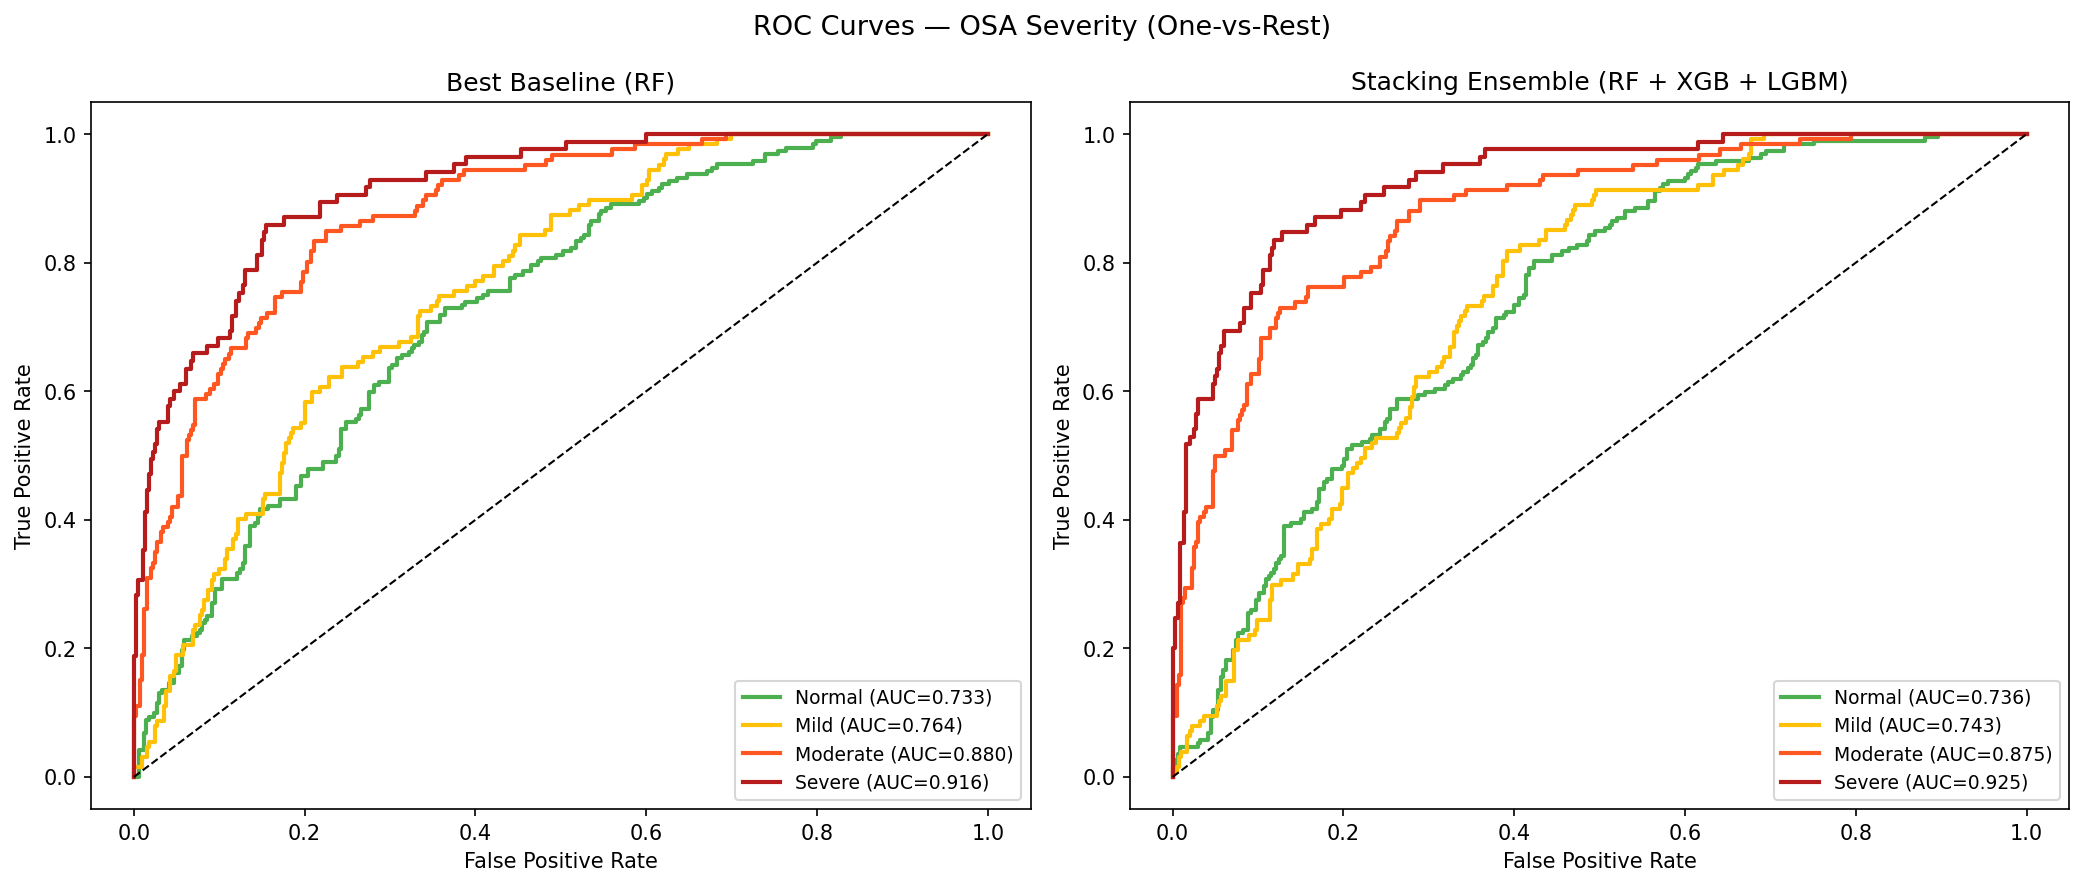
\includegraphics[width=\textwidth]{images/resultats/roc_curves.png}
\caption[Courbes ROC de la prédiction de sévérité]%
        {Courbes ROC en un-contre-tous, meilleure ligne de base et ensemble.}
\label{fig:roc-osa}
\end{figure}

\begin{samepage}
\noindent\textbf{Avertissement sur les étiquettes.} Les figures produites par le script
d'origine portaient des étiquettes d'axes erronées : l'encodeur de classes les trie par
ordre alphabétique, si bien que l'ordre effectif des indices est \emph{Léger, Modéré,
Normal, Sévère} et non l'ordre de sévérité utilisé dans le code. Le défaut ne touchait que
l'affichage (les prédictions du système sont correctes) mais il a été corrigé dans
le script, et les matrices présentées ici ont été recalculées avec l'ordre exact.
\end{samepage}

\subsubsection{Explicabilité des prédictions}

\paragraph{Choix de la méthode}

Les méthodes d'explication se répartissent selon plusieurs axes
(figure~\ref{fig:xai-taxo}). Notre besoin est précis : expliquer une prédiction unique
(explication locale), pour un modèle d'ensemble (méthode agnostique ou spécifique
aux arbres), de manière exacte et reproductible.

\begin{figure}[H]
\centering
\begin{tikzpicture}[
    x=1cm,y=1cm,
    racine/.style = {rectangle,rounded corners=2pt,draw=hypnoblue!65,fill=hypnolight,
                     align=center,font=\small\bfseries,minimum height=0.8cm,text width=3.6cm},
    branche/.style= {rectangle,rounded corners=2pt,draw=hypnoblue!50,fill=white,
                     align=center,font=\scriptsize\bfseries,minimum height=0.75cm,text width=3.0cm},
    feuille/.style= {rectangle,rounded corners=2pt,draw=hypnogray!45,fill=white,
                     anchor=west,align=left,font=\scriptsize,
                     minimum height=0.62cm,text width=3.35cm,inner xsep=5pt},
    ret/.style    = {rectangle,rounded corners=2pt,draw=hypnored!80,fill=hypnored!8,
                     anchor=west,align=left,font=\scriptsize\bfseries,
                     minimum height=0.62cm,text width=3.35cm,inner xsep=5pt},
    li/.style     = {hypnoblue!55,line width=0.7pt},
    bus/.style    = {hypnogray!55,line width=0.7pt},
  ]

  % ── Racine et deux branches ───────────────────────────────────────────────
  \node[racine]  (r)   at (7.4,3.55) {Méthodes d'explication};
  \node[branche] (spe) at (2.6,2.05) {Spécifiques\\à une architecture};
  \node[branche] (agn) at (10.4,2.05) {Agnostiques\\au modèle};

  \draw[li] (r.west)  -- ++(-1.2,0) |- (spe.north);
  \draw[li] (r.east)  -- ++(1.2,0)  |- (agn.north);

  % ── Feuilles : méthodes spécifiques ───────────────────────────────────────
  \node[feuille] (sal)  at (2.15, 0.95) {Cartes de saillance~\cite{simonyan2014}};
  \node[feuille] (gcam) at (2.15, 0.15) {Grad-CAM~\cite{selvaraju2017}};
  \node[feuille] (ig)   at (2.15,-0.65) {Gradients intégrés~\cite{sundararajan2017}};
  \node[feuille] (att)  at (2.15,-1.45) {Poids d'attention~\cite{bahdanau2015}};

  \draw[bus] (1.75,1.60) -- (1.75,-1.45);
  \foreach \n in {sal,gcam,ig,att}
    \draw[bus] (1.75,0 |- \n.west) -- (\n.west);
  \draw[bus] (1.75,1.60) -- (2.6,1.60) -- (2.6,1.68);

  % ── Feuilles : méthodes agnostiques ───────────────────────────────────────
  \node[feuille] (lime) at (9.95, 0.95) {LIME~\cite{ribeiro2016}};
  \node[ret]     (shap) at (9.95, 0.15) {SHAP~\cite{lundberg2017}};
  \node[feuille] (perm) at (9.95,-0.65) {Importance par permutation};
  \node[feuille] (pdp)  at (9.95,-1.45) {Dépendance partielle};

  \draw[bus] (9.55,1.60) -- (9.55,-1.45);
  \foreach \n in {lime,shap,perm,pdp}
    \draw[bus] (9.55,0 |- \n.west) -- (\n.west);
  \draw[bus] (9.55,1.60) -- (10.4,1.60) -- (10.4,1.68);

  \node[font=\scriptsize\itshape,text=hypnogray,anchor=north] at (7.0,-2.10)
       {la méthode encadrée en rouge est celle retenue dans ce travail};

\end{tikzpicture}
\vspace{0.3cm}
\caption[Taxonomie des méthodes d'explication]%
        {Taxonomie des principales méthodes d'explication, selon leur dépendance à
         l'architecture du modèle.}
\label{fig:xai-taxo}
\end{figure}

Les valeurs de Shapley~\cite{shapley1953}, transposées à l'apprentissage automatique par
SHAP~\cite{lundberg2017}, répondent à ce cahier des charges. Elles décomposent la
prédiction en contributions additives par variable, avec des propriétés d'unicité
démontrées. Leur variante dédiée aux arbres~\cite{lundberg2020} les calcule en temps
polynomial plutôt qu'exponentiel, ce qui les rend applicables en production.

\begin{figure}[H]
\centering
\begin{tikzpicture}[
    x=1cm,y=1cm,
    barP/.style = {fill=hypnored!70,draw=hypnored,line width=0.4pt},
    barN/.style = {fill=hypnoblue!55,draw=hypnoblue,line width=0.4pt},
    et/.style   = {font=\scriptsize,anchor=east,text=hypnogray},
    va/.style   = {font=\scriptsize,text=hypnogray},
  ]

  % Axe de référence
  \draw[hypnogray!45,dashed,line width=0.6pt] (0,0.5) -- (0,-4.6);
  \node[font=\scriptsize\itshape,text=hypnogray,anchor=south] at (0,0.55)
       {valeur de base $E[f(x)]$};

  % Contributions successives
  \draw[barP] (0,-0.2)   rectangle (3.2,-0.65);
  \node[et] at (-0.15,-0.42) {index de fragmentation};
  \node[va,anchor=west] at (3.35,-0.42) {$+$};

  \draw[barP] (3.2,-1.0) rectangle (5.0,-1.45);
  \node[et] at (-0.15,-1.22) {\% du temps sous \SI{90}{\percent}};
  \node[va,anchor=west] at (5.15,-1.22) {$+$};

  \draw[barP] (5.0,-1.8) rectangle (6.1,-2.25);
  \node[et] at (-0.15,-2.02) {indice de masse corporelle};
  \node[va,anchor=west] at (6.25,-2.02) {$+$};

  \draw[barN] (5.3,-2.6) rectangle (6.1,-3.05);
  \node[et] at (-0.15,-2.82) {\% de sommeil profond};
  \node[va,anchor=west] at (6.25,-2.82) {$-$};

  \draw[barN] (4.9,-3.4) rectangle (5.3,-3.85);
  \node[et] at (-0.15,-3.62) {latence d'endormissement};
  \node[va,anchor=west] at (6.25,-3.62) {$-$};

  % Prédiction finale
  \draw[hypnored,line width=1pt,dashed] (4.9,-4.1) -- (4.9,-4.6);
  \node[font=\scriptsize\bfseries,text=hypnored,anchor=north] at (4.9,-4.65)
       {prédiction : sévère};

  \node[font=\scriptsize\itshape,text=hypnogray,anchor=west] at (7.0,-1.6)
       {\begin{minipage}{5.2cm}\raggedright
        Chaque barre est la contribution $\phi_i$ d'une variable.
        Les contributions rouges poussent vers une sévérité plus élevée,
        les bleues vers une sévérité moindre. Leur somme relie exactement
        la valeur de base à la prédiction.
        \end{minipage}};

\end{tikzpicture}
\vspace{0.2cm}
\caption[Lecture en cascade d'une explication SHAP]%
        {Lecture en cascade d'une explication SHAP : la propriété d'additivité relie
         la valeur de base à la prédiction individuelle.}
\label{fig:shap-cascade}
\end{figure}

\paragraph{Mise en œuvre et résultats}

Les attributions sont calculées sur le modèle à gradient boosté, puis triées par
contribution absolue décroissante. Les dix variables dominantes sont restituées au
praticien, séparées en facteurs aggravants et protecteurs.

\begin{figure}[H]
\centering
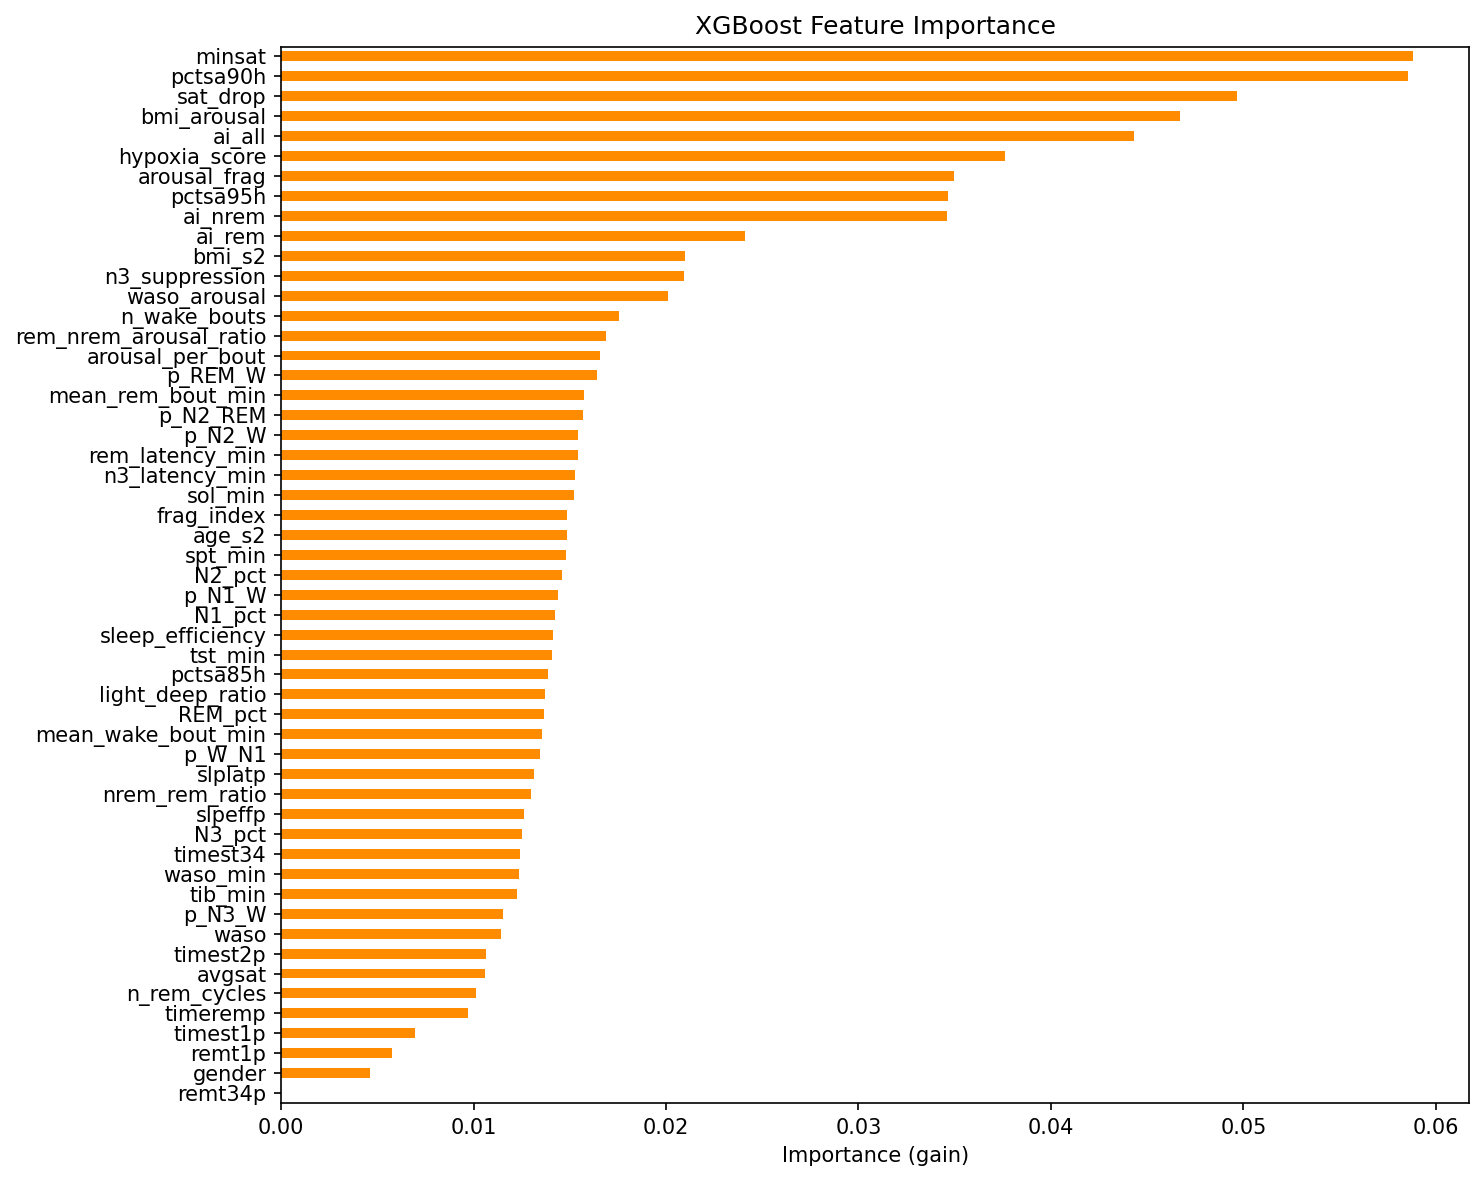
\includegraphics[width=0.86\textwidth]{images/resultats/xgb_feature_importance.png}
\caption[Importance globale des variables]%
        {Importance des variables du modèle de sévérité, mesurée par le gain.}
\label{fig:importance}
\end{figure}

Les variables les plus influentes relèvent de l'oxymétrie et des index d'éveil, ce qui est
physiologiquement cohérent : ce sont les conséquences les plus directes des événements
respiratoires. Les marqueurs d'architecture du sommeil (fragmentation, proportion de
sommeil profond, durée d'éveil intra-sommeil) viennent ensuite et apportent
l'information complémentaire qui justifie la démarche.

Ces attributions expliquent le \emph{modèle}, non le
\emph{phénomène}. Une contribution élevée signale une forte influence sur la prédiction,
en aucun cas un lien de causalité. Le compte rendu remis au praticien porte cette mention.

Un second point tient à la méthode : la prédiction est rendue par un ensemble hétérogène,
mais l'explication est calculée sur un modèle à arbres entraîné sur les mêmes données. Ce
dédoublement permet d'obtenir des attributions exactes en temps polynomial, là où
expliquer directement l'ensemble aurait imposé une approximation par échantillonnage.
L'explication décrit donc un modèle très proche du modèle décisionnel, non ce modèle
lui-même.

\subsubsection{Synthèse méthodologique}
\label{sec:synthese}

Trois limites affectent la portée des résultats obtenus depuis le sprint 1.

\subparagraph{Un découpage au niveau des époques.} Les douze modèles de base ont été évalués
sur un découpage aléatoire des \num{195130} fenêtres, sans tenir compte du sujet dont
elles proviennent. Comme chaque sujet contribue environ un millier d'époques, dont
\SI{80}{\percent} atterrissent dans l'ensemble d'entraînement, le modèle a vu, pour
presque chaque époque de test, d'autres époques du même patient et de la même nuit. Les
métriques mesurent donc la capacité à classer \emph{une époque inconnue d'un patient
connu}, et non \emph{un patient inconnu}.

\subparagraph{Deux protocoles non comparables.} Les ensembles, eux, ont été évalués sur un
découpage par sujets. Il en résulte que les valeurs du tableau~\ref{tab:ensembles} et
celles du tableau~\ref{tab:12modeles} ne sont pas directement comparables. Le
mémoire ne présente donc pas le passage de \SI{91,66}{\percent} à \SI{96,93}{\percent}
comme un gain de l'empilement, car ce serait une comparaison invalide. Plus gênant : les
modèles de base ayant été entraînés sur un découpage par époques, ils avaient déjà
rencontré des fenêtres appartenant aux sujets que le protocole d'empilement considère
comme non vus.

\subparagraph{Un corpus restreint et filtré.} Le sous-corpus de 196 sujets représente
\SI{3,4}{\percent} de la cohorte disponible, et il a été constitué par filtrage sur la
complétude du montage plutôt que par tirage aléatoire.

\medskip
\noindent
Ces trois limites se renforcent mutuellement et pointent vers un même correctif : une
ré-évaluation complète sur un découpage par sujets unique, appliqué de façon
identique aux modèles de base et aux ensembles. Ce travail, qui ne nécessite aucune
modification des architectures, constitue la première des perspectives.

\subsection{Revue du sprint}

Ce sprint a produit les quatre ensembles de classification et le modèle de prédiction de
sévérité, accompagné de son mécanisme d'explication.

Deux résultats nuancés en ressortent. L'empilement dépasse le meilleur modèle isolé sur
les quatre configurations de classification, mais ne dépasse le vote moyen que sur trois
d'entre elles. Et sur la prédiction de sévérité, il \emph{dégrade} légèrement la meilleure
ligne de base, faute de diversité entre trois modèles tous fondés sur des arbres.

Le modèle de sévérité atteint \SI{57,0}{\percent} d'exactitude sur quatre classes, avec
plus de \SI{95}{\percent} des prédictions dans la bonne classe ou une classe adjacente,
la statistique qui compte cliniquement.

Les modèles sont désormais complets. Le sprint suivant les expose à travers une interface
applicative et un poste de travail utilisable par un praticien.

% ---------------------------------------------------------------------------
\section{Sprint 4 : Service d'inférence et poste de travail}
\label{sec:sprint4}
% ---------------------------------------------------------------------------

Les trois premiers sprints ont produit des modèles. Ce quatrième sprint, qui clôt la
release, les rend utilisables : il expose une interface applicative sécurisée et construit
le poste de travail du praticien, depuis le dépôt d'un enregistrement jusqu'au rapport de
sévérité expliqué.

\subsection{Objectif du sprint}

L'objectif était de franchir le pas du \emph{carnet d'expérimentation} vers le
\emph{service}. Trois exigences le structuraient.

La première était la disponibilité des modèles. Chargés naïvement à chaque
requête, les modèles imposeraient plusieurs secondes de latence : ils devaient donc être
conservés en mémoire entre deux appels.

La deuxième était la sécurisation des accès. Une plateforme manipulant des
données de santé ne peut être ouverte : authentification, jetons signés et cloisonnement
des rôles devaient être posés dès ce sprint.

La troisième était l'ergonomie du parcours. Une analyse dure plusieurs dizaines
de secondes ; l'interface devait guider le praticien et le tenir informé sans jamais le
laisser devant un écran muet.

\subsection{Sprint Backlog}

Le sprint a embarqué seize récits pour 80 points de complexité
(tableau~\ref{tab:bl-s4}).

\begin{table}[H]
\centering\small
\renewcommand{\arraystretch}{1.15}
\begin{tabular}{@{}c|L{2.5cm}|L{4.6cm}|L{4.6cm}|c@{}}
\hline
\ligneentete \entete{ID} & \entete{Module} & \entete{R\'ecit utilisateur} & \entete{T\^aches} & \entete{Estim.} \\
\hline
\multirow{3}{*}{US-26\,\`a\,29} & \multirow{3}{=}{Authentification} & \multirow{3}{=}{En tant qu'utilisateur, je veux me connecter et acc\'eder aux fonctions de mon r\^ole} & Hacher les mots de passe avec sel al\'eatoire & \multirow{3}{*}{15 pts} \\
 &  &  & D\'elivrer un jeton sign\'e \`a expiration &  \\
 &  &  & V\'erifier le r\^ole sur chaque route prot\'eg\'ee &  \\
\hline
\multirow{3}{*}{US-09\,\`a\,12} & \multirow{3}{=}{Service d'inf\'erence} & \multirow{3}{=}{En tant que m\'edecin, je veux lancer une analyse en choisissant la configuration adapt\'ee \`a mon montage} & Exposer les routes d'analyse et d'inspection & \multirow{3}{*}{19 pts} \\
 &  &  & Mettre les mod\`eles en cache m\'emoire &  \\
 &  &  & Calculer les m\'etriques AASM &  \\
\hline
\multirow{3}{*}{US-17\,\`a\,20} & \multirow{3}{=}{Rapport de s\'ev\'erit\'e} & \multirow{3}{=}{En tant que m\'edecin, je veux saisir les donn\'ees cliniques et obtenir un rapport expliqu\'e} & Cr\'eer le formulaire clinique & \multirow{3}{*}{23 pts} \\
 &  &  & Analyser les rapports externes import\'es &  \\
 &  &  & Produire l'interpr\'etation automatique &  \\
\hline
\multirow{3}{*}{US-21\,\`a\,23} & \multirow{3}{=}{Visualisation} & \multirow{3}{=}{En tant que m\'edecin, je veux visualiser l'hypnogramme et suivre la progression de l'analyse} & Tracer l'hypnogramme interactif & \multirow{3}{*}{18 pts} \\
 &  &  & Superposer saturation et densit\'e d'\'ev\'enements &  \\
 &  &  & Afficher l'\'ecran de progression &  \\
\hline
\multirow{1}{*}{US-40} & \multirow{1}{=}{Export} & \multirow{1}{=}{En tant que m\'edecin, je veux exporter les marqueurs calcul\'es} & Produire les exports tabulaire et balis\'e & \multirow{1}{*}{5 pts} \\
\hline
\end{tabular}
\caption{Sprint Backlog --- Sprint 4}
\label{tab:bl-s4}
\end{table}

\subsection{Analyse}

\subsubsection{Diagramme des cas d'utilisation}

\begin{figure}[H]
\centering
\begin{tikzpicture}[
    x=1cm,y=1cm,
    uc/.style     = {ellipse, draw=hypnoblue!60, fill=hypnolight,
                     align=center, font=\scriptsize, text width=2.7cm,
                     inner sep=1.5pt, minimum height=1.0cm},
    ucp/.style    = {ellipse, draw=hypnored!70, fill=hypnored!7,
                     align=center, font=\scriptsize\bfseries, text width=2.7cm,
                     inner sep=1.5pt, minimum height=1.0cm},
    lien/.style   = {hypnogray!75, line width=0.55pt},
    rel/.style    = {-{Latex[length=2mm]}, hypnoblue!70, line width=0.5pt, dashed},
    et/.style     = {font=\tiny\itshape, text=hypnoblue!85, fill=white, inner sep=1pt},
    nomact/.style = {font=\scriptsize\bfseries, align=center, text width=2.2cm},
  ]

  \tikzset{acteur/.pic={
      \draw[hypnoblue,line width=0.8pt] (0,0) circle (0.17);
      \draw[hypnoblue,line width=0.8pt] (0,-0.17) -- (0,-0.66);
      \draw[hypnoblue,line width=0.8pt] (-0.28,-0.34) -- (0.28,-0.34);
      \draw[hypnoblue,line width=0.8pt] (0,-0.66) -- (-0.24,-1.04);
      \draw[hypnoblue,line width=0.8pt] (0,-0.66) -- (0.24,-1.04);}}

  \draw[hypnoblue!55,line width=0.9pt,rounded corners=3pt]
       (3.6,-5.4) rectangle (12.6,2.4);
  \node[font=\small\bfseries,text=hypnoblue,anchor=north west] at (3.85,2.25)
       {Poste de travail du médecin};

  \node[uc]  (auth) at (5.8, 1.4)  {S'authentifier};
  \node[ucp] (ana)  at (5.8,-0.6)  {Analyser un\\enregistrement};
  \node[uc]  (exp)  at (5.8,-3.9)  {Exporter les\\marqueurs};

  \node[uc]  (cfg)  at (10.3, 1.3) {Choisir montage\\et granularité};
  \node[uc]  (vis)  at (10.3,-0.2) {Visualiser\\l'hypnogramme};
  \node[uc]  (met)  at (10.3,-1.7) {Consulter les\\métriques AASM};
  \node[uc]  (sev)  at (10.3,-3.2) {Obtenir le rapport\\de sévérité};
  \node[uc]  (imp)  at (10.3,-4.7) {Importer un\\rapport externe};

  \pic at (1.5,0.9) {acteur};
  \node[nomact,anchor=north] at (1.5,0.25) {Médecin};

  \draw[lien] (1.9,0.55) -- (auth.west);
  \draw[lien] (1.9,0.55) -- (ana.west);
  \draw[lien] (1.9,0.55) -- (exp.west);

  \draw[rel] (ana) -- node[et,pos=0.58] {$\ll$include$\gg$} (cfg);
  \draw[rel] (ana) -- node[et,pos=0.6]  {$\ll$include$\gg$} (vis);
  \draw[rel] (ana) -- node[et,pos=0.6]  {$\ll$include$\gg$} (met);
  \draw[rel] (sev) -- node[et,pos=0.5,above]  {$\ll$extend$\gg$} (met);
  \draw[rel] (imp) -- node[et,pos=0.5,below]  {$\ll$extend$\gg$} (sev);
  \draw[rel] (ana) -- node[et,pos=0.55] {$\ll$include$\gg$} (auth);

\end{tikzpicture}
\caption{Diagramme des cas d'utilisation du sprint 4 --- poste de travail du médecin}
\label{fig:uc-s4}
\end{figure}

\subsubsection{Description textuelle des cas d'utilisation}

\begin{casutilisation}{Description textuelle du cas « Analyser un enregistrement »}
Titre & Analyser un enregistrement \\ \hline
Acteurs & Médecin du sommeil, moteur d'inférence \\ \hline
Description & Produire l'hypnogramme et les métriques d'une nuit à partir d'un fichier
d'enregistrement brut \\ \hline
Préconditions & Le médecin est authentifié ; sa licence est valide ; il dispose d'un
fichier au format EDF \\ \hline
Scénario de base &
\begin{minipage}[t]{\linewidth}
\begin{enumerate}[leftmargin=1.1em,itemsep=1pt,topsep=3pt]
  \item Le médecin choisit le montage disponible, à deux ou cinq dérivations.
  \item Il choisit la granularité de classification, à trois ou cinq stades.
  \item Il dépose le fichier d'enregistrement.
  \item Le système décode le fichier, résout les dérivations et prétraite le signal.
  \item Le moteur classe chaque époque et le système calcule les métriques.
  \item Le système affiche l'hypnogramme, les métriques et les alertes cliniques.
\end{enumerate}
\end{minipage} \\ \hline
Scénario alternatif &
\begin{minipage}[t]{\linewidth}
\begin{itemize}[leftmargin=1.1em,itemsep=1pt,topsep=3pt]
  \item \textbf{3a} --- Le fichier n'est pas au format attendu : le dépôt est refusé.
  \item \textbf{4a} --- Une dérivation est absente : repli documenté, l'analyse aboutit.
  \item \textbf{4b} --- L'enregistrement est trop court : interruption avec message.
\end{itemize}
\end{minipage}
\end{casutilisation}

\subsection{Conception}

\subsubsection{Diagrammes de séquence objet}

Les figures~\ref{fig:seq-auth} et~\ref{fig:seq-analyse} décrivent les deux enchaînements
structurants du sprint : l'ouverture de session et l'analyse d'un enregistrement.

\begin{figure}[H]
\centering
\resizebox{0.98\textwidth}{!}{%
\begin{sequencediagram}
  \newthread[hypnolight]{u}{\scriptsize Praticien}
  \newinst[2.2]{f}{\scriptsize Client web}
  \newinst[2.2]{a}{\scriptsize Interface applicative}
  \newinst[2.2]{d}{\scriptsize Base de données}

  \begin{call}{u}{\scriptsize saisit ses identifiants}{f}{}
  \end{call}
  \begin{call}{f}{\scriptsize demande de jeton}{a}{\scriptsize jeton et profil}
    \begin{call}{a}{\scriptsize recherche du compte}{d}{\scriptsize empreinte}
    \end{call}
    \begin{sdblock}{\scriptsize Vérifications}{\scriptsize mot de passe, statut, licence}
      \begin{call}{a}{\scriptsize horodate la connexion}{d}{}
      \end{call}
      \begin{call}{a}{\scriptsize journalise l'accès}{d}{}
      \end{call}
    \end{sdblock}
  \end{call}
  \begin{call}{f}{\scriptsize conserve le jeton}{f}{}
  \end{call}
  \begin{call}{f}{\scriptsize ouvre l'espace de travail}{u}{}
  \end{call}
\end{sequencediagram}}
\caption[Séquence d'authentification]%
        {Ouverture de session et délivrance du jeton.}
\label{fig:seq-auth}
\end{figure}

\begin{figure}[H]
\centering
\resizebox{0.98\textwidth}{!}{%
\begin{sequencediagram}
  \newthread[hypnolight]{u}{\scriptsize Praticien}
  \newinst[1.8]{f}{\scriptsize Client web}
  \newinst[1.8]{a}{\scriptsize Interface applicative}
  \newinst[1.8]{m}{\scriptsize Moteur d'inférence}
  \newinst[1.8]{d}{\scriptsize Base de données}
  \newinst[1.8]{s}{\scriptsize Stockage objet}

  \begin{call}{u}{\scriptsize dépose le fichier}{f}{}
  \end{call}
  \begin{call}{f}{\scriptsize demande d'analyse}{a}{\scriptsize stades et métriques}
    \begin{call}{a}{\scriptsize prétraitement}{m}{\scriptsize tenseur d'époques}
    \end{call}
    \begin{call}{a}{\scriptsize classification}{m}{\scriptsize séquence de stades}
    \end{call}
    \begin{call}{a}{\scriptsize métriques AASM}{m}{\scriptsize indicateurs}
    \end{call}
  \end{call}
  \begin{call}{f}{\scriptsize affiche l'hypnogramme}{u}{}
  \end{call}
  \begin{call}{f}{\scriptsize enregistre l'examen}{a}{\scriptsize identifiant}
    \begin{call}{a}{\scriptsize insertion}{d}{}
    \end{call}
  \end{call}
  \begin{sdblock}{\scriptsize Arrière-plan}{\scriptsize sans blocage de l'interface}
    \begin{call}{f}{\scriptsize transfert du fichier}{a}{\scriptsize référence}
      \begin{call}{a}{\scriptsize dépôt}{s}{\scriptsize clé d'objet}
      \end{call}
      \begin{call}{a}{\scriptsize mise à jour}{d}{}
      \end{call}
    \end{call}
  \end{sdblock}
\end{sequencediagram}}
\caption[Séquence d'analyse d'un enregistrement]%
        {Analyse d'un enregistrement : les résultats précèdent l'archivage.}
\label{fig:seq-analyse}
\end{figure}

La particularité de cet enchaînement tient à l'ordre des opérations : les résultats sont
affichés au praticien \emph{avant} que l'archivage du fichier, mis en place au sprint
suivant, ne soit terminé.

\subsection{Réalisation}

\subsubsection{Organisation de l'interface applicative}

L'interface applicative est bâtie sur FastAPI, choisi pour son modèle asynchrone, sa
validation déclarative des données et la génération automatique de sa documentation. Le
code est réparti en modules à responsabilité unique.

\begin{table}[H]
\centering

\small
\begin{tabular}{@{}lrL{8.3cm}@{}}
\toprule
\textbf{Module} & \textbf{Lignes} & \textbf{Responsabilité} \\
\midrule
\texttt{main.py}          & 695 & Point d'entrée, routes métier et d'administration,
                                  migration au démarrage, journalisation \\
\texttt{ml\_routes.py}    & 984 & Routes d'inférence : analyse, extraction de
                                  marqueurs, prédiction de sévérité, lecture de
                                  fichiers externes \\
\texttt{ml\_models.py}    & 117 & Définition des trois architectures de réseaux \\
\texttt{preprocessing.py} & 199 & Décodage EDF, résolution des dérivations, calcul
                                  des métriques AASM \\
\texttt{osa\_predictor.py}& 113 & Chargement des modèles de sévérité, prédiction et
                                  attribution des contributions \\
\texttt{db\_models.py}    & 113 & Modèle de données et relations \\
\texttt{schemas.py}       & 163 & Schémas de validation des entrées et sorties \\
\texttt{auth.py}          &  51 & Jetons, empreintes de mots de passe, dépendance
                                  d'authentification \\
\texttt{b2\_storage.py}   & 121 & Client de stockage objet, dépôt et signature des
                                  liens \\
\texttt{database.py}      &  19 & Connexion et session \\
\bottomrule
\end{tabular}
\caption{Modules de l'interface applicative}
\label{tab:modules}
\end{table}

Deux mécanismes transversaux sont à signaler. Le premier est la migration
au démarrage : le schéma ayant évolué au fil des sprints, l'application exécute à son
lancement une série d'ajouts de colonnes conditionnels, ce qui permet de déployer une
nouvelle version sur une base existante sans intervention manuelle. Le second est la
signature des liens à la sérialisation, développée au sprint suivant.

\subsubsection{Points d'entrée}

L'interface expose trente-six routes réparties en six domaines. L'authentification en
compte deux : \texttt{/token} délivre le jeton, \texttt{/users/me} renvoie le profil de
l'appelant. L'administration en compte neuf, toutes réservées au rôle administrateur,
qui couvrent le cycle de vie des comptes médecins et la réinitialisation de leur mot de
passe, les établissements, les statistiques globales, et le journal d'audit avec son
export.

Quatre routes servent le registre des patients et huit les examens, toutes réservées au
rôle médecin : création et mise à jour d'un examen, dépôt de l'enregistrement brut, de
l'hypnogramme, de sa version annotée et du compte rendu de sévérité, puis les
annotations portées à l'époque. Six autres portent la collaboration, de l'annuaire des
confrères aux messages d'un fil.

Les sept dernières sont celles du service de modèles : contrôle de santé, inspection des
canaux d'un fichier, analyse d'un enregistrement, extraction des marqueurs, prédiction de
la sévérité dans ses deux variantes et lecture d'un rapport externe. La documentation
OpenAPI correspondante est produite automatiquement (figure~\ref{fig:swagger}).

La version livrée présente ici une faiblesse : les routes d'inférence
ne sont pas protégées par le contrôle d'accès. Ce choix, initialement fait pour faciliter
les essais pendant la mise au point, n'a pas été rétabli. Un appelant non authentifié peut
donc soumettre un enregistrement à l'analyse. Aucune donnée patient n'est exposée (ces
routes ne lisent ni n'écrivent en base) mais elles consomment des ressources de calcul.
L'ajout de la dépendance d'authentification, qui tient en une ligne par route, figure parmi
les corrections à apporter avant toute mise en service réelle.

\capturefig{swagger}{0.9}{Documentation OpenAPI générée automatiquement}{fig:swagger}

\subsubsection{Sécurité des accès}

\begin{table}[H]
\centering

\small
\begin{tabular}{@{}L{3.2cm}L{5.3cm}L{5.5cm}@{}}
\toprule
\textbf{Mécanisme} & \textbf{Principe} & \textbf{Menace couverte} \\
\midrule
Empreintes de mots de passe &
Fonction de dérivation lente avec sel aléatoire par compte &
Compromission de la base : les mots de passe restent inexploitables \\
\addlinespace[3pt]
Jetons signés &
Jeton porteur signé, transmis à chaque appel, contenant l'identité et le rôle &
Usurpation : toute altération invalide la signature \\
\addlinespace[3pt]
Contrôle d'accès par rôle &
Vérification du rôle et de la propriété de la ressource sur chaque route protégée &
Élévation de privilège et accès aux patients d'un confrère \\
\addlinespace[3pt]
Liens d'accès signés &
Les références de fichiers sont converties en URL signées valables 24 heures &
Fuite de données : aucun objet n'est accessible sans signature valide \\
\bottomrule
\end{tabular}
\caption{Mécanismes de sécurité et menaces couvertes}
\label{tab:secu}
\end{table}

Les mots de passe sont hachés par bcrypt, dont le sel aléatoire par compte
interdit les tables précalculées. Les jetons sont signés en HMAC-SHA256 et portent
l'adresse de l'utilisateur, son rôle et une date d'expiration fixée à sept jours. Le
contrôle d'accès superpose deux niveaux : le rôle est vérifié en tête de route, la
propriété de la ressource l'est ensuite.

\subsubsection{Poste de travail du praticien}

L'interface est une application monopage React, construite par Vite, organisée en
composants regroupés par domaine fonctionnel.

\begin{table}[H]
\centering

\small
\begin{tabular}{@{}lrL{8.0cm}@{}}
\toprule
\textbf{Composant} & \textbf{Lignes} & \textbf{Rôle} \\
\midrule
\texttt{AnalysisResults} & 1134 & Restitution complète : hypnogramme, métriques,
                                  marqueurs, formulaire clinique, rapport de sévérité \\
\texttt{PatientList}     &  993 & Registre des patients, historique des examens,
                                  documents archivés \\
\texttt{CustomOSA}       &  658 & Prédiction à partir d'une saisie manuelle ou d'un
                                  rapport importé \\
\texttt{Hypnogram}       &  552 & Tracé interactif de l'hypnogramme, de la saturation
                                  et de la densité d'événements \\
\texttt{DoctorList}      &  539 & Administration des comptes et des licences \\
\texttt{DeveloperPipeline} & 497 & Visualisation de la chaîne de traitement \\
\texttt{LandingPage}     &  406 & Page publique et authentification \\
\texttt{AnalysisWizard}  &  428 & Assistant d'analyse en quatre étapes \\
\texttt{HospitalsDashboard} & 233 & Gestion des établissements \\
\texttt{ConsultationsView}  & 198 & Boîte de réception des sollicitations \\
\texttt{AuditLogsDashboard} & 194 & Consultation et export du journal \\
\texttt{CollaborationChat}  & 171 & Fil de discussion rattaché à un examen \\
\bottomrule
\end{tabular}
\caption{Principaux composants de l'interface}
\label{tab:composants}
\end{table}

Le parcours principal se déroule en quatre étapes : le praticien déclare le montage
disponible, puis la granularité souhaitée, dépose le fichier, et consulte les résultats.
Chaque étape n'expose qu'une seule décision, assortie d'une recommandation par défaut.

\capturefig{wizard-1}{0.86}{Assistant d'analyse, étape 1 : déclaration du montage}{fig:wizard1}

\capturefig{wizard-2}{0.86}{Assistant d'analyse, étape 2 : granularité de classification}{fig:wizard2}

Pendant le traitement, un écran de progression affiche les tracés physiologiques et
détaille les cinq étapes du pipeline. Ce retour visuel a une fonction précise : une
interface muette pendant plusieurs dizaines de secondes laisserait croire à un blocage.

\capturefig{progression}{0.86}{Écran de progression du traitement}{fig:progression}

La page de résultats superpose sur un même axe temporel l'hypnogramme prédit, la courbe de
saturation et la densité d'événements respiratoires. Cette superposition est le choix de
visualisation le plus utile de l'interface : elle permet de constater directement qu'une
désaturation coïncide avec une sortie de sommeil paradoxal, ce que trois graphiques séparés
ne montreraient pas.

\capturefig{resultats}{0.92}{Restitution des résultats d'analyse}{fig:resultats}

Un second parcours permet une prédiction sans enregistrement, à partir d'une saisie manuelle
ou d'un rapport externe importé. Cette voie répond à un usage réel : disposer d'un compte
rendu produit par un autre laboratoire sans avoir accès au signal brut.

\capturefig{custom-osa}{0.86}{Prédiction de sévérité à partir d'une saisie manuelle}{fig:customosa}

\subsection{Revue du sprint}

Ce sprint a transformé des modèles de laboratoire en un service utilisable. L'interface
applicative expose les routes d'inférence, conserve les modèles en mémoire et protège les
routes métier par un double contrôle de rôle et de propriété. Le poste de travail guide
l'analyse en quatre décisions et restitue les résultats sur un axe temporel unique.

Une faiblesse a été identifiée et documentée : les routes d'inférence ne sont pas
authentifiées.

% ---------------------------------------------------------------------------
\section{Revue de la release 2}
\label{sec:revue-release2}
% ---------------------------------------------------------------------------

\subsection{Incrément livré}

La release a livré ses 122 points en deux sprints, dont 80 pour le seul sprint~4.
L'incrément démontré lors de la revue est récapitulé au tableau~\ref{tab:revue-r2}.

\begin{table}[H]
\centering\small
\renewcommand{\arraystretch}{1.2}
\begin{tabular}{@{}L{3.6cm}|L{8.6cm}|c@{}}
\hline
\ligneentete \entete{Élément attendu} & \entete{Réalisation} & \entete{État} \\
\hline
Ensembles de classification & Quatre ensembles par empilement, supérieurs au meilleur
modèle isolé sur les quatre configurations & \checkmark \\
\hline
Modèle de sévérité & Quatre classes, 53 variables : \SI{57,0}{\percent} d'exactitude et
plus de \SI{95}{\percent} des prédictions à un cran près & \checkmark \\
\hline
Explication des prédictions & Attributions par valeurs de Shapley, restituées en facteurs
aggravants et protecteurs & \checkmark \\
\hline
Interface applicative & Jetons signés, contrôle des rôles, modèles conservés en mémoire ;
routes d'inférence non authentifiées & avec réserve \\
\hline
Poste de travail & Assistant d'analyse en quatre étapes, restitution sur un axe temporel
unique, prédiction sans enregistrement & \checkmark \\
\hline
\end{tabular}
\caption{Revue de la release 2 : incrément attendu et incrément livré}
\label{tab:revue-r2}
\end{table}

\subsection{Rétrospective}

La rétrospective de la release a retenu trois enseignements.

\subparagraph{Comparer à la bonne référence.} Confronter l'empilement au vote moyen, et pas
seulement au meilleur modèle isolé, a montré que son apport est réel mais modeste. Sur la
prédiction de sévérité, il dégrade même légèrement la meilleure ligne de base, faute de
diversité entre les modèles combinés.

\subparagraph{Unifier les protocoles d'évaluation.} La synthèse méthodologique du sprint~3
a établi que modèles de base et ensembles n'ont pas été évalués sur le même découpage. La
correction, une ré-évaluation sur un découpage par sujets unique, ne touche aucune
architecture ; elle constitue la première des perspectives du projet.

\subparagraph{Documenter la dette technique.} Les routes d'inférence, laissées ouvertes
pour faciliter la mise au point, n'ont pas été protégées par le contrôle d'accès. La
faiblesse est identifiée, et sa correction, d'une ligne par route, figure parmi les
préalables à toute mise en service.

\sectionsansnum{Conclusion}

La deuxième release a livré la première version de \hypnoria{} exploitable par un
praticien. Les modèles de classification coopèrent au sein de quatre ensembles, la sévérité
du syndrome d'apnées est prédite en quatre classes et chaque prédiction est accompagnée de
ses facteurs explicatifs ; le tout est accessible depuis un poste de travail qui guide
l'analyse en quatre décisions.

Il manque cependant à cet outil ce qui en ferait un système d'information clinique : la
mémoire des patients et de leurs examens, la gouvernance des accès et les moyens du travail
à plusieurs. C'est l'objet de la troisième et dernière release.
    % Release 2 : sprints 3 et 4
\chapter{Release 3 : Plateforme clinique et industrialisation}
\label{chap:release3}

\sectionsansnum{Introduction}

Ce chapitre présente la troisième et dernière release, menée de la semaine 17 à la
semaine 24. Elle transforme l'outil d'analyse livré par la release précédente en une
plateforme clinique complète : dossier patient persistant, archivage sécurisé, gouvernance
multi-établissements, collaboration entre praticiens, restitution documentaire et
déploiement reproductible. Comme les précédents, le chapitre présente la release, détaille
ses deux sprints et en dresse la revue.

% ---------------------------------------------------------------------------
\section{Présentation de la release}
\label{sec:release3}
% ---------------------------------------------------------------------------

\subsection{Objectif de la release}

La troisième release vise à livrer une plateforme prête à être déployée en
contexte clinique. Les fonctions d'analyse ne changent plus ; ce qui s'ajoute, c'est tout ce
qui permet de les exploiter durablement, à plusieurs et en confiance. Le sprint~5 dote la
plateforme d'une mémoire et d'une gouvernance ; le sprint~6 couvre la collaboration, la
production du compte rendu et l'industrialisation du déploiement.

\subsection{Backlog de la release}

Avec trente-deux récits et 160 points de complexité, cette release est la plus volumineuse
du projet (tableau~\ref{tab:rel3}). Elle solde le backlog du produit : à son terme, les
soixante récits ont été livrés.

\begin{table}[H]
\centering\small
\renewcommand{\arraystretch}{1.2}
\begin{tabular}{@{}L{1.4cm}|L{3.0cm}|L{5.4cm}|L{2.7cm}|c@{}}
\hline
\ligneentete \entete{Sprint} & \entete{Période} & \entete{Objectif du sprint} &
\entete{Récits} & \entete{Pts} \\
\hline
Sprint 5 & 18 mai -- 14 juin &
Transformer l'outil d'analyse en plateforme gouvernée et traçable &
US-30 à 35, 37 à 39, 43 à 51 & 77 \\
\hline
Sprint 6 & 15 juin -- 12 juil. &
Couvrir le travail à plusieurs, la restitution documentaire et la reproductibilité &
US-24, 25, 36, 41, 42, 52 à 60 & 83 \\
\hline
\multicolumn{3}{@{}r|}{\textbf{Total de la release}} & \textbf{32 récits} & \textbf{160} \\
\hline
\end{tabular}
\caption{Backlog de la release 3}
\label{tab:rel3}
\end{table}

\noindent
L'incrément attendu en fin de release est la plateforme complète, conteneurisée et vérifiée
automatiquement à chaque livraison.

% ---------------------------------------------------------------------------
\section{Sprint 5 : Dossier patient et gouvernance}
\label{sec:sprint5}
% ---------------------------------------------------------------------------

Le sprint précédent a livré un outil d'analyse. Ce cinquième sprint, qui ouvre la release,
en fait un système d'information clinique : les examens sont rattachés à des patients, les
fichiers volumineux archivés hors base, et la plateforme ouverte à plusieurs établissements
sous le contrôle d'un administrateur.

\subsection{Objectif du sprint}

Trois exigences structuraient ce sprint.

La première était la persistance. Une analyse sans dossier n'a pas d'usage
clinique : il fallait rattacher chaque examen à un patient, conserver l'historique et
cloisonner les données de chaque praticien.

La deuxième était le traitement des fichiers volumineux. Un enregistrement pèse
plusieurs centaines de mégaoctets. Le conserver en base aurait dégradé les sauvegardes et
les temps de réponse sans bénéfice transactionnel.

La troisième était la gouvernance. Ouvrir la plateforme à plusieurs centres
suppose de pouvoir créer des comptes, en révoquer l'accès sans détruire de données, et
tracer les actions sensibles.

\subsection{Sprint Backlog}

Le sprint a embarqué dix-huit récits pour 77 points de complexité
(tableau~\ref{tab:bl-s5}).

\begin{table}[H]
\centering\small
\renewcommand{\arraystretch}{1.15}
\begin{tabular}{@{}c|L{2.5cm}|L{4.6cm}|L{4.6cm}|c@{}}
\hline
\ligneentete \entete{ID} & \entete{Module} & \entete{R\'ecit utilisateur} & \entete{T\^aches} & \entete{Estim.} \\
\hline
\multirow{3}{*}{US-31\,\`a\,35} & \multirow{3}{=}{Dossier patient} & \multirow{3}{=}{En tant que m\'edecin, je veux constituer et suivre mon registre de patients} & Mod\'eliser patients et examens & \multirow{3}{*}{19 pts} \\
 &  &  & Cr\'eer le registre et l'historique &  \\
 &  &  & Cloisonner les donn\'ees par praticien &  \\
\hline
\multirow{3}{*}{US-37\,\`a\,39} & \multirow{3}{=}{Archivage cloud} & \multirow{3}{=}{En tant que syst\`eme, je veux archiver les fichiers volumineux sans bloquer l'interface} & Int\'egrer le client de stockage objet & \multirow{3}{*}{18 pts} \\
 &  &  & Transf\'erer en arri\`ere-plan avec suivi &  \\
 &  &  & D\'elivrer des liens sign\'es \`a dur\'ee limit\'ee &  \\
\hline
\multirow{3}{*}{US-43\,\`a\,47} & \multirow{3}{=}{Comptes et licences} & \multirow{3}{=}{En tant qu'administrateur, je veux g\'erer le cycle de vie des comptes m\'edecins} & Cr\'eer et lister les comptes & \multirow{3}{*}{21 pts} \\
 &  &  & Suspendre, r\'eactiver et fixer l'\'ech\'eance &  \\
 &  &  & G\'erer les \'etablissements de rattachement &  \\
\hline
\multirow{3}{*}{US-30, 48\,\`a\,51} & \multirow{3}{=}{Tra\c{c}abilit\'e} & \multirow{3}{=}{En tant qu'administrateur, je veux tracer et exporter les actions sensibles} & Journaliser auteur, horodatage et adresse & \multirow{3}{*}{19 pts} \\
 &  &  & Appliquer statut et licence \`a la connexion &  \\
 &  &  & Exporter le journal au format tabulaire &  \\
\hline
\end{tabular}
\caption{Sprint Backlog --- Sprint 5}
\label{tab:bl-s5}
\end{table}

\subsection{Analyse}

\subsubsection{Diagramme des cas d'utilisation}

\begin{figure}[H]
\centering
\begin{tikzpicture}[
    x=1cm,y=1cm,
    uc/.style     = {ellipse, draw=hypnoblue!60, fill=hypnolight,
                     align=center, font=\scriptsize, text width=2.7cm,
                     inner sep=1.5pt, minimum height=1.0cm},
    ucp/.style    = {ellipse, draw=hypnored!70, fill=hypnored!7,
                     align=center, font=\scriptsize\bfseries, text width=2.7cm,
                     inner sep=1.5pt, minimum height=1.0cm},
    lien/.style   = {hypnogray!75, line width=0.55pt},
    rel/.style    = {-{Latex[length=2mm]}, hypnoblue!70, line width=0.5pt, dashed},
    et/.style     = {font=\tiny\itshape, text=hypnoblue!85, fill=white, inner sep=1pt},
    nomact/.style = {font=\scriptsize\bfseries, align=center, text width=2.2cm},
  ]

  \tikzset{acteur/.pic={
      \draw[hypnoblue,line width=0.8pt] (0,0) circle (0.17);
      \draw[hypnoblue,line width=0.8pt] (0,-0.17) -- (0,-0.66);
      \draw[hypnoblue,line width=0.8pt] (-0.28,-0.34) -- (0.28,-0.34);
      \draw[hypnoblue,line width=0.8pt] (0,-0.66) -- (-0.24,-1.04);
      \draw[hypnoblue,line width=0.8pt] (0,-0.66) -- (0.24,-1.04);}}

  \draw[hypnoblue!55,line width=0.9pt,rounded corners=3pt]
       (3.9,-5.4) rectangle (11.9,2.4);
  \node[font=\small\bfseries,text=hypnoblue,anchor=north west] at (4.15,2.25)
       {Système d'information clinique};

  \node[uc]  (pat) at (6.1, 1.4)  {Gérer ses\\patients};
  \node[ucp] (exa) at (6.1,-0.3)  {Constituer le\\dossier d'examen};
  \node[uc]  (arc) at (6.1,-2.2)  {Archiver les\\pièces};
  \node[uc]  (tab) at (6.1,-4.1)  {Consulter son\\tableau de bord};

  \node[uc]  (com) at (9.9, 1.4)  {Gérer les comptes\\et licences};
  \node[uc]  (eta) at (9.9,-0.3)  {Gérer les\\établissements};
  \node[uc]  (aud) at (9.9,-2.2)  {Consulter le\\journal d'audit};
  \node[uc]  (sta) at (9.9,-4.1)  {Suivre l'activité\\de la plateforme};

  \pic at (1.6,0.9) {acteur};
  \node[nomact,anchor=north] at (1.6,0.25) {Médecin};

  \pic at (14.0,0.9) {acteur};
  \node[nomact,anchor=north] at (14.0,0.25) {Administrateur};

  \foreach \c in {pat,exa,arc,tab} \draw[lien] (2.0,0.55) -- (\c.west);
  \foreach \c in {com,eta,aud,sta} \draw[lien] (13.6,0.55) -- (\c.east);

  \draw[rel] (exa) -- node[et,pos=0.5] {$\ll$include$\gg$} (arc);

\end{tikzpicture}
\caption{Diagramme des cas d'utilisation du sprint 5 --- dossier patient et gouvernance}
\label{fig:uc-s5}
\end{figure}

\subsubsection{Description textuelle des cas d'utilisation}

\begin{casutilisation}{Description textuelle du cas « Gérer le cycle de vie d'un compte »}
Titre & Gérer le cycle de vie d'un compte médecin \\ \hline
Acteur & Administrateur \\ \hline
Description & Créer un compte praticien, en suspendre ou réactiver l'accès, fixer son
échéance de licence et le rattacher à un établissement \\ \hline
Préconditions & L'administrateur est authentifié \\ \hline
Scénario de base &
\begin{minipage}[t]{\linewidth}
\begin{enumerate}[leftmargin=1.1em,itemsep=1pt,topsep=3pt]
  \item L'administrateur ouvre le registre des médecins.
  \item Il crée un compte en renseignant identité, adresse et échéance de licence.
  \item Le système vérifie l'unicité de l'adresse et hache le mot de passe initial.
  \item Le système journalise la création.
  \item L'administrateur peut ensuite suspendre, réactiver ou prolonger le compte.
\end{enumerate}
\end{minipage} \\ \hline
Scénario alternatif &
\begin{minipage}[t]{\linewidth}
\begin{itemize}[leftmargin=1.1em,itemsep=1pt,topsep=3pt]
  \item \textbf{3a} --- L'adresse est déjà enregistrée : la création est refusée.
  \item \textbf{5a} --- Le praticien a perdu son accès : réinitialisation avec mot de
        passe temporaire.
\end{itemize}
\end{minipage}
\end{casutilisation}

\subsection{Conception}

\subsubsection{Diagramme d'états}

Un examen traverse une succession d'états. Cette modélisation explicite un point important :
un examen reste consultable même si l'archivage échoue, car les résultats d'analyse sont
stockés en base indépendamment des fichiers.

\begin{figure}[H]
\centering
\begin{tikzpicture}[
    x=1cm,y=1cm,
    st/.style   = {rectangle,rounded corners=5pt,draw=hypnoblue!65,fill=hypnolight,
                   align=center,font=\scriptsize,minimum height=0.9cm,text width=2.3cm},
    stf/.style  = {rectangle,rounded corners=5pt,draw=hypnored!70,fill=hypnored!7,
                   align=center,font=\scriptsize,minimum height=0.9cm,text width=2.3cm},
    fl/.style   = {-{Latex[length=2mm]},hypnoblue!75,line width=0.7pt},
    tr/.style   = {font=\tiny\itshape,text=hypnogray,fill=white,inner sep=1.5pt},
  ]

  \fill[hypnoblue] (0,0) circle (0.14);

  \node[st]  (cre) at (2.5,0)   {Créé};
  \node[st]  (ana) at (6.0,0)   {Analysé};
  \node[st]  (arc) at (9.5,0)   {Archivé};
  \node[stf] (eva) at (13.0,0)  {Évalué};
  \node[st]  (ann) at (9.5,-2.3){Annoté};
  \node[stf] (deg) at (6.0,-2.3){Archivage\\en échec};

  \draw[fl] (0.16,0) -- node[tr,above] {dépôt du fichier} (cre);
  \draw[fl] (cre) -- node[tr,above] {classification} (ana);
  \draw[fl] (ana) -- node[tr,above] {transfert réussi} (arc);
  \draw[fl] (arc) -- node[tr,above] {prédiction} (eva);
  \draw[fl] (arc) -- node[tr,right,pos=0.5] {annotation} (ann);
  \draw[fl] (ana) -- node[tr,right,pos=0.5] {transfert échoué} (deg);
  \draw[fl] (deg) -- node[tr,below] {nouvelle tentative} (ann);

  \fill[hypnoblue] (13.0,-2.3) circle (0.19);
  \fill[white]     (13.0,-2.3) circle (0.135);
  \fill[hypnoblue] (13.0,-2.3) circle (0.09);
  \draw[fl] (eva) -- node[tr,right,pos=0.5] {compte rendu} (13.0,-2.11);
  \draw[fl] (ann) -- node[tr,pos=0.72,below right] {prédiction} (eva.south west);

\end{tikzpicture}
\vspace{0.3cm}
\caption[Cycle de vie d'un examen]%
        {États successifs d'un examen ; l'échec d'archivage ne bloque pas
         l'exploitation des résultats.}
\label{fig:etats}
\end{figure}

\subsection{Réalisation}

\subsubsection{Persistance et cloisonnement}

Le modèle de données repose sur huit tables, présentées au chapitre~\ref{chap:analyse}. Le
rattachement direct du patient à son praticien référent fonde le cloisonnement : chaque route
vérifie, après le rôle, que la ressource demandée appartient bien à l'appelant. Un médecin ne
peut donc pas accéder au dossier d'un confrère, même en devinant un identifiant.

\subsubsection{Archivage sur stockage objet}

Les fichiers volumineux sont confiés à un service de stockage objet compatible avec
l'interface S3. Chaque objet est rangé dans un préfixe portant le nom du patient et nommé
selon le motif \texttt{patient\_date\_alea}, ce qui rend l'arborescence lisible depuis la
console du fournisseur sans consulter la base.

Le point central de cette réalisation est le transfert en arrière-plan. Attendre
la fin du téléversement avant d'afficher les résultats aurait immobilisé le praticien pendant
plusieurs minutes. L'enchaînement retenu est donc : l'analyse est exécutée, les résultats sont
affichés, l'examen est créé en base, puis le transfert démarre sans bloquer l'interface. Une
vignette flottante affiche la progression et disparaît quelques secondes après son achèvement.

Un échec de transfert n'interrompt rien : il est signalé dans la vignette, et l'examen reste
pleinement exploitable.

Les liens d'accès aux fichiers sont signés et expirent au bout de vingt-quatre heures.
Une subtilité a été traitée : les enregistrements et les fichiers tabulaires sont servis avec
une en-tête forçant le téléchargement, tandis que les images et les comptes rendus restent
affichables dans le navigateur.

Ces références ne sont jamais transmises telles quelles : les schémas de sortie déclarent un
validateur qui intercepte toute référence de fichier au moment de composer la réponse et la
remplace par un lien signé. Aucune route ne peut donc divulguer une
référence brute par inadvertance, puisque la conversion est appliquée par le schéma et non par
la route.

\subsubsection{Administration et cycle de vie des licences}

Un compte peut être actif, suspendu ou en attente, et porte une date d'échéance. Ces trois
conditions sont évaluées à chaque ouverture de session, avec un message distinct pour chacune,
de sorte que le praticien sache s'il doit contacter son administrateur ou renouveler son
abonnement.

Ce dispositif permet de révoquer un accès sans détruire de données, ce qui est la
seule manière acceptable de gérer une fin de contrat sur un système qui héberge des dossiers
médicaux.

\capturefig{admin-medecins}{0.9}{Registre des médecins et gestion des licences}{fig:adminmed}

\capturefig{admin-hopitaux}{0.9}{Gestion des établissements rattachés}{fig:adminhop}

\subsubsection{Traçabilité}

Chaque action sensible inscrit dans le journal son auteur, son rôle, son horodatage, la nature
de l'action et l'adresse d'origine. Sont journalisées les connexions, les créations de compte,
les modifications de statut et les réinitialisations de mot de passe. Le journal est exportable
au format tabulaire pour un contrôle externe.

La table est délibérément dénormalisée : elle recopie l'adresse et le rôle plutôt que de
référencer le compte, afin que la trace survive à la disparition de celui-ci.

\capturefig{audit}{0.9}{Journal d'audit : consultation et export}{fig:audit}

\subsubsection{Limites au regard du règlement européen}

Le système n'est pas conforme au règlement général sur la protection des données. Trois
écarts subsistent.

Les données patient ne sont pas chiffrées au repos : elles reposent sur le chiffrement
offert par le service de stockage et par le système de fichiers de la base, sans couche
applicative supplémentaire. Le droit à l'effacement n'est pas outillé : aucune
procédure n'efface un patient et ses fichiers archivés en une opération. Enfin, aucune
durée de conservation n'est définie ni appliquée.

Ces trois points relèvent d'un travail de mise en conformité qui dépasse le périmètre d'un
projet de fin d'études, mais qu'une mise en service réelle imposerait.

\subsection{Revue du sprint}

Ce sprint a doté la plateforme d'une mémoire et d'une gouvernance. Les examens sont désormais
rattachés à des patients, les fichiers volumineux archivés hors base et accessibles uniquement
par des liens signés, et l'administrateur dispose des outils nécessaires pour ouvrir la
plateforme à plusieurs établissements.

Un principe directeur guide ces choix : ne jamais faire attendre le
praticien, et ne jamais laisser un incident technique compromettre l'exploitation d'un examen.

Le sprint suivant, dernier du projet, couvre le travail à plusieurs, la restitution
documentaire et l'industrialisation du déploiement.

% ---------------------------------------------------------------------------
\section{Sprint 6 : Collaboration, restitution et industrialisation}
\label{sec:sprint6}
% ---------------------------------------------------------------------------

Ce dernier sprint couvre trois volets complémentaires : le travail à plusieurs, la
production du document qui sort du système, et l'industrialisation du déploiement.

\subsection{Objectif du sprint}

L'interprétation d'un enregistrement difficile se fait rarement seul. Le premier objectif
était donc de permettre à un praticien de solliciter un confrère, en gardant la
discussion attachée à l'examen concerné.

Le deuxième objectif était la restitution. Un système d'aide au diagnostic dont on ne
peut rien extraire n'a pas d'usage : il fallait produire un compte rendu composable, adapté au
destinataire.

Le troisième était l'industrialisation : rendre le déploiement reproductible et
vérifier automatiquement qu'une modification ne casse rien.

\subsection{Sprint Backlog}

Le sprint a embarqué quatorze récits pour 83 points de complexité
(tableau~\ref{tab:bl-s6}).

\begin{table}[H]
\centering\small
\renewcommand{\arraystretch}{1.15}
\begin{tabular}{@{}c|L{2.5cm}|L{4.6cm}|L{4.6cm}|c@{}}
\hline
\ligneentete \entete{ID} & \entete{Module} & \entete{R\'ecit utilisateur} & \entete{T\^aches} & \entete{Estim.} \\
\hline
\multirow{3}{*}{US-53\,\`a\,55} & \multirow{3}{=}{Collaboration} & \multirow{3}{=}{En tant que m\'edecin, je veux solliciter un confr\`ere sur un examen pr\'ecis} & Mod\'eliser fils et messages rattach\'es \`a un examen & \multirow{3}{*}{18 pts} \\
 &  &  & Cr\'eer l'interface de discussion &  \\
 &  &  & Centraliser les sollicitations re\c{c}ues &  \\
\hline
\multirow{3}{*}{US-24, 25, 42} & \multirow{3}{=}{Annotation et normes} & \multirow{3}{=}{En tant que m\'edecin, je veux annoter une \'epoque et situer chaque m\'etrique par rapport aux normes} & Enregistrer les notes horodat\'ees \`a l'\'epoque & \multirow{3}{*}{15 pts} \\
 &  &  & Synchroniser l'hypnogramme annot\'e &  \\
 &  &  & Comparer les m\'etriques aux valeurs de r\'ef\'erence &  \\
\hline
\multirow{3}{*}{US-36, 41} & \multirow{3}{=}{Restitution} & \multirow{3}{=}{En tant que m\'edecin, je veux composer et exporter mon compte rendu} & S\'electionner les sections \`a inclure & \multirow{3}{*}{13 pts} \\
 &  &  & Produire le document pagin\'e &  \\
 &  &  & Afficher le tableau de bord de la patient\`ele &  \\
\hline
\multirow{5}{*}{US-52, 56\,\`a\,60} & \multirow{5}{=}{Industrialisation} & \multirow{5}{=}{En tant que d\'eveloppeur, je veux un d\'eploiement reproductible et v\'erifi\'e automatiquement} & Conteneuriser les trois services & \multirow{5}{*}{37 pts} \\
 &  &  & Orchestrer la pile en une commande &  \\
 &  &  & Automatiser contr\^oles et construction d'images &  \\
 &  &  & Traduire l'interface et ajouter le th\`eme sombre &  \\
 &  &  & Visualiser la cha\^ine de traitement des mod\`eles &  \\
\hline
\end{tabular}
\caption{Sprint Backlog --- Sprint 6}
\label{tab:bl-s6}
\end{table}

\subsection{Analyse}

\subsubsection{Diagramme des cas d'utilisation}

\begin{figure}[H]
\centering
\begin{tikzpicture}[
    x=1cm,y=1cm,
    uc/.style     = {ellipse, draw=hypnoblue!60, fill=hypnolight,
                     align=center, font=\scriptsize, text width=2.7cm,
                     inner sep=1.5pt, minimum height=1.0cm},
    ucp/.style    = {ellipse, draw=hypnored!70, fill=hypnored!7,
                     align=center, font=\scriptsize\bfseries, text width=2.7cm,
                     inner sep=1.5pt, minimum height=1.0cm},
    lien/.style   = {hypnogray!75, line width=0.55pt},
    rel/.style    = {-{Latex[length=2mm]}, hypnoblue!70, line width=0.5pt, dashed},
    et/.style     = {font=\tiny\itshape, text=hypnoblue!85, fill=white, inner sep=1pt},
    nomact/.style = {font=\scriptsize\bfseries, align=center, text width=2.2cm},
  ]

  \tikzset{acteur/.pic={
      \draw[hypnoblue,line width=0.8pt] (0,0) circle (0.17);
      \draw[hypnoblue,line width=0.8pt] (0,-0.17) -- (0,-0.66);
      \draw[hypnoblue,line width=0.8pt] (-0.28,-0.34) -- (0.28,-0.34);
      \draw[hypnoblue,line width=0.8pt] (0,-0.66) -- (-0.24,-1.04);
      \draw[hypnoblue,line width=0.8pt] (0,-0.66) -- (0.24,-1.04);}}

  \draw[hypnoblue!55,line width=0.9pt,rounded corners=3pt]
       (3.9,-4.6) rectangle (12.0,2.4);
  \node[font=\small\bfseries,text=hypnoblue,anchor=north west] at (4.15,2.25)
       {Collaboration et restitution};

  \node[ucp] (col) at (6.2, 1.2)  {Solliciter un\\confrère};
  \node[uc]  (msg) at (10.0, 1.2) {Échanger des\\messages};
  \node[uc]  (rec) at (10.0,-0.4) {Consulter la boîte\\de réception};
  \node[uc]  (ann) at (6.2,-1.1)  {Annoter une\\époque};
  \node[uc]  (nor) at (10.0,-2.0) {Comparer aux\\normes};
  \node[ucp] (pdf) at (6.2,-3.3)  {Composer le\\compte rendu};
  \node[uc]  (sec) at (10.0,-3.6) {Choisir les\\sections};

  \pic at (1.6,0.7) {acteur};
  \node[nomact,anchor=north] at (1.6,0.05) {Médecin};

  \pic at (14.1,0.7) {acteur};
  \node[nomact,anchor=north] at (14.1,0.05) {Confrère};

  \foreach \c in {col,ann,pdf} \draw[lien] (2.0,0.35) -- (\c.west);
  \draw[lien] (13.7,0.35) -- (msg.east);
  \draw[lien] (13.7,0.35) -- (rec.east);

  \draw[rel] (col) -- node[et,pos=0.5] {$\ll$include$\gg$} (msg);
  \draw[rel] (col) -- node[et,pos=0.6] {$\ll$extend$\gg$} (rec);
  \draw[rel] (ann) -- node[et,pos=0.6] {$\ll$extend$\gg$} (nor);
  \draw[rel] (pdf) -- node[et,pos=0.55] {$\ll$include$\gg$} (sec);

\end{tikzpicture}
\caption{Diagramme des cas d'utilisation du sprint 6 --- collaboration et restitution}
\label{fig:uc-s6}
\end{figure}

\subsubsection{Description textuelle des cas d'utilisation}

\begin{casutilisation}{Description textuelle du cas « Solliciter un confrère »}
Titre & Solliciter un confrère sur un examen \\ \hline
Acteurs & Médecin demandeur, confrère sollicité \\ \hline
Description & Ouvrir une discussion rattachée à un examen afin de recueillir un avis, en
conservant le contexte clinique \\ \hline
Préconditions & Les deux praticiens sont authentifiés ; l'examen existe \\ \hline
Scénario de base &
\begin{minipage}[t]{\linewidth}
\begin{enumerate}[leftmargin=1.1em,itemsep=1pt,topsep=3pt]
  \item Le médecin ouvre la fiche du patient et sélectionne l'examen.
  \item Il demande la liste des confrères disponibles.
  \item Il sélectionne un confrère et rédige sa demande.
  \item Le système crée le fil, ou réutilise celui qui existe déjà, et enregistre le message.
  \item Le confrère consulte sa boîte de réception et répond dans le même fil.
\end{enumerate}
\end{minipage} \\ \hline
Scénario alternatif &
\begin{minipage}[t]{\linewidth}
\begin{itemize}[leftmargin=1.1em,itemsep=1pt,topsep=3pt]
  \item \textbf{4a} --- Un fil existe déjà entre ces deux praticiens sur cet examen : le
        message y est ajouté plutôt que d'ouvrir un doublon.
\end{itemize}
\end{minipage}
\end{casutilisation}

\subsection{Conception}

\subsubsection{Diagramme de séquence objet}

La figure~\ref{fig:seq-s6} détaille la sollicitation d'un confrère. Deux points la
caractérisent. L'ouverture du fil est idempotente : l'interface applicative recherche
d'abord une discussion existante entre les deux praticiens sur le même examen, et ne la
crée qu'à défaut. L'envoi d'un message est ensuite une opération distincte, soumise à la
vérification que l'appelant participe bien au fil.

\begin{figure}[H]
\centering
\resizebox{0.98\textwidth}{!}{%
\begin{sequencediagram}
  \newthread[hypnolight]{u}{\scriptsize Médecin}
  \newinst[1.8]{f}{\scriptsize Client web}
  \newinst[1.8]{a}{\scriptsize Interface applicative}
  \newinst[1.8]{d}{\scriptsize Base de données}
  \newinst[1.8]{c}{\scriptsize Confrère}

  \begin{call}{u}{\scriptsize sollicite un confrère}{f}{}
  \end{call}
  \begin{call}{f}{\scriptsize liste des confrères}{a}{\scriptsize praticiens}
    \begin{call}{a}{\scriptsize recherche}{d}{}
    \end{call}
  \end{call}
  \begin{call}{f}{\scriptsize ouverture du fil}{a}{\scriptsize identifiant du fil}
    \begin{sdblock}{\scriptsize Contrôle}{\scriptsize fil existant réutilisé, sinon créé}
      \begin{call}{a}{\scriptsize recherche ou création}{d}{}
      \end{call}
    \end{sdblock}
  \end{call}
  \begin{call}{f}{\scriptsize envoi du message}{a}{\scriptsize message}
    \begin{call}{a}{\scriptsize vérifie la participation}{a}{}
    \end{call}
    \begin{call}{a}{\scriptsize insertion}{d}{}
    \end{call}
  \end{call}
  \begin{call}{c}{\scriptsize consulte sa boîte de réception}{a}{\scriptsize fils et messages}
    \begin{call}{a}{\scriptsize fils du praticien}{d}{}
    \end{call}
  \end{call}
  \begin{call}{c}{\scriptsize répond dans le fil}{a}{\scriptsize message}
    \begin{call}{a}{\scriptsize insertion}{d}{}
    \end{call}
  \end{call}
\end{sequencediagram}}
\caption{Diagramme de séquence objet du sprint 6 --- sollicitation d'un confrère}
\label{fig:seq-s6}
\end{figure}

\subsection{Réalisation}

\subsubsection{Consultations confraternelles}

Un fil de discussion est rattaché à un examen et à exactement deux praticiens. L'intérêt de ce
dispositif est que la discussion reste attachée à l'examen : le correspondant dispose du
contexte sans qu'il faille le lui transmettre. Une vue centralisée rassemble toutes les
sollicitations reçues.

\capturefig{consultation}{0.86}{Fil de discussion rattaché à un examen}{fig:consultation}

\subsubsection{Annotation et comparaison aux normes}

Le praticien peut annoter une époque précise de l'hypnogramme ; ses observations sont
conservées et peuvent être synchronisées vers le dossier, ce qui archive l'hypnogramme annoté
aux côtés des autres pièces.

Chaque métrique AASM est par ailleurs accompagnée de sa plage de référence et d'une comparaison
aux valeurs de la cohorte. Une valeur hors norme est signalée visuellement, et une liste
d'alertes cliniques reprend en clair les anomalies détectées.

\subsubsection{Production du compte rendu}

Le compte rendu est produit côté client : les sections retenues sont converties en images par
capture du rendu, puis assemblées dans un document paginé. Cette approche garantit que le
document reproduit exactement ce que le praticien a validé à l'écran, sans qu'un moteur de
rendu distinct puisse introduire un écart.

Le praticien choisit les sections à inclure : hypnogramme, métriques AASM, classe de sévérité,
facteurs explicatifs, tracés bruts et comparaison aux normes. Cette composition à la carte
répond à des destinataires différents : un confrère n'attend pas le même document qu'un
dossier d'assurance. Le document est ensuite archivé au même titre que les autres pièces.

\capturefig{rapport}{0.78}{Compte rendu clinique généré}{fig:rapport}

\subsubsection{Multilinguisme et thème sombre}

L'interface est intégralement traduite en français et en anglais, les chaînes étant centralisées
dans un catalogue unique et la bascule immédiate. Un thème sombre est également disponible,
adapté à la lecture nocturne : un praticien qui interprète un enregistrement le fait
rarement en plein jour.

\capturefig{dark}{0.86}{Tableau de bord du médecin en thème sombre}{fig:dark}

\subsubsection{Conteneurisation}

La pile est décrite par un fichier d'orchestration unique qui déclare trois services.

\begin{table}[H]
\centering

\small
\begin{tabular}{@{}lllL{5.4cm}@{}}
\toprule
\textbf{Service} & \textbf{Image de base} & \textbf{Port} & \textbf{Particularité} \\
\midrule
Base de données & \texttt{postgres:15-alpine} & 5432 &
Volume persistant, sonde de disponibilité \\
\addlinespace[2pt]
Interface applicative & \texttt{python:3.10-slim} & 8000 &
PyTorch en version processeur installé en premier \\
\addlinespace[2pt]
Serveur web & \texttt{node:20-alpine} puis \texttt{nginx:alpine} & 80 &
Construction en deux étapes, redirection du routage client \\
\bottomrule
\end{tabular}
\caption{Services de la pile conteneurisée}
\label{tab:services}
\end{table}

Le fichier de construction de l'interface applicative comporte une particularité :
PyTorch y est installé depuis l'index dédié aux processeurs, \emph{avant} les
autres dépendances. Sans cette précaution, l'installation télécharge plusieurs gigaoctets de
bibliothèques inutiles en déploiement (l'inférence en production s'exécutant sur processeur)
et fait échouer la construction sur une machine de développement.

La sonde de disponibilité de la base est également indispensable : sans elle, l'interface
applicative démarrerait avant que la base n'accepte les connexions et échouerait à créer son
schéma.

\subsubsection{Intégration continue}

Une chaîne d'intégration continue s'exécute à chaque livraison sur la branche principale et à
chaque proposition de fusion.

\begin{table}[H]
\centering

\small
\begin{tabular}{@{}lL{10.4cm}@{}}
\toprule
\textbf{Travail} & \textbf{Étapes} \\
\midrule
Interface applicative &
Installation des dépendances avec PyTorch en version processeur ; contrôle syntaxique
de tous les modules ; démarrage d'une instance PostgreSQL de service ; démarrage réel
de l'application ; vérification du schéma OpenAPI et de la présence des points
d'entrée attendus ; contrôle du cloisonnement des rôles \\
\addlinespace[3pt]
Interface utilisateur &
Installation reproductible des dépendances ; analyse statique ; construction de
production ; publication du bundle en tant qu'artefact \\
\addlinespace[3pt]
Images de conteneur &
Construction des deux images avec cache de couches, conditionnée à la réussite des
deux travaux précédents \\
\bottomrule
\end{tabular}
\caption{Travaux de la chaîne d'intégration continue}
\label{tab:ci}
\end{table}

Le travail portant sur l'interface applicative va au-delà du contrôle syntaxique : il
démarre réellement l'application contre une base éphémère, puis exerce trois
vérifications de comportement. Un appel sans jeton doit recevoir un refus d'authentification ;
une connexion administrateur doit délivrer un jeton ; et ce jeton d'administrateur, présenté au
registre des patients, doit recevoir un refus d'autorisation. Ces trois assertions couvrent
l'essentiel du cloisonnement des rôles et échoueraient immédiatement si une dépendance de
sécurité venait à disparaître au fil d'une modification.

\capturefig{ci}{0.9}{Exécution de la chaîne d'intégration continue}{fig:ci}

\subsection{Revue du sprint}

Ce dernier sprint a complété la plateforme sur ses trois derniers volets. Les praticiens peuvent
solliciter un confrère sans quitter le contexte de l'examen, composer un compte rendu adapté à
son destinataire, et travailler dans la langue et le thème de leur choix.

La pile est entièrement conteneurisée et vérifiée par une chaîne d'intégration continue qui
démarre réellement l'application et contrôle le cloisonnement des rôles.

% ---------------------------------------------------------------------------
\section{Revue de la release 3}
\label{sec:revue-release3}
% ---------------------------------------------------------------------------

\subsection{Incrément livré}

La release a livré ses 160 points en deux sprints, portant le total livré à 358 points sur
les six sprints du projet (tableau~\ref{tab:revue-r3}).

\begin{table}[H]
\centering\small
\renewcommand{\arraystretch}{1.2}
\begin{tabular}{@{}L{3.6cm}|L{9.4cm}|c@{}}
\hline
\ligneentete \entete{Élément attendu} & \entete{Réalisation} & \entete{État} \\
\hline
Dossier patient & Registre des patients, historique des examens, cloisonnement des
données par praticien & \checkmark \\
\hline
Archivage & Stockage objet, transfert en arrière-plan, liens signés valables vingt-quatre
heures & \checkmark \\
\hline
Gouvernance & Cycle de vie des comptes et des licences, établissements, journal d'audit
exportable & \checkmark \\
\hline
Collaboration et restitution & Fils de discussion rattachés aux examens, annotation,
compte rendu composable & \checkmark \\
\hline
Industrialisation & Pile de trois conteneurs, intégration continue, interface bilingue et
thème sombre & \checkmark \\
\hline
\end{tabular}
\caption{Revue de la release 3 : incrément attendu et incrément livré}
\label{tab:revue-r3}
\end{table}

\subsection{Validation fonctionnelle}
\label{sec:validation}

En complément de la chaîne d'intégration continue, une campagne de scénarios fonctionnels
a été exécutée manuellement à chaque fin de sprint. Le tableau~\ref{tab:tests} en présente
l'état sur la version livrée au terme de la release.

\begin{table}[H]
\centering

\small
\begin{tabular}{@{}clL{7.2cm}c@{}}
\toprule
\textbf{N\textsuperscript{o}} & \textbf{Scénario} & \textbf{Critère de réussite} &
\textbf{État} \\
\midrule
1 & Connexion valide & Jeton délivré, espace de travail ouvert & \checkmark \\
2 & Connexion refusée & Compte suspendu ou licence expirée rejeté avec message
    distinct & \checkmark \\
3 & Cloisonnement des rôles & Un médecin n'atteint aucune route d'administration &
    \checkmark \\
4 & Cloisonnement des patients & Un médecin n'accède pas au dossier d'un confrère &
    \checkmark \\
5 & Analyse complète & Enregistrement déposé, hypnogramme et métriques affichés &
    \checkmark \\
6 & Montage incomplet & Dérivation absente : repli appliqué, analyse aboutie &
    \checkmark \\
7 & Fichier invalide & Format non reconnu refusé avec message explicite & \checkmark \\
8 & Prédiction de sévérité & Classe, probabilités et facteurs restitués & \checkmark \\
9 & Import de rapport externe & Formulaire prérempli depuis un fichier tabulaire ou
    balisé & \checkmark \\
10 & Archivage en arrière-plan & Résultats affichés avant la fin du transfert &
    \checkmark \\
11 & Échec d'archivage & Transfert interrompu : examen consultable, erreur signalée &
    \checkmark \\
12 & Lien expiré & Lien réutilisé après échéance : accès refusé & \checkmark \\
13 & Annotation d'époque & Note enregistrée et retrouvée au rechargement & \checkmark \\
14 & Consultation confraternelle & Message émis par un praticien, reçu par l'autre &
    \checkmark \\
15 & Compte rendu & Document produit avec les seules sections sélectionnées &
    \checkmark \\
16 & Journal d'audit & Actions sensibles tracées et exportées & \checkmark \\
17 & Bascule linguistique & Aucune chaîne non traduite sur le parcours principal &
    \checkmark \\
18 & Démarrage de la pile & Trois services opérationnels en une commande & \checkmark \\
\bottomrule
\end{tabular}
\caption{Scénarios de validation fonctionnelle}
\label{tab:tests}
\end{table}

Cette approche a une limite : une campagne manuelle n'est ni reproductible
ni exhaustive, et elle ne protège pas contre les régressions entre deux exécutions. Les trois
assertions automatisées constituent un premier filet de sécurité, mais une véritable couverture
de tests reste à construire.

\subsection{Rétrospective}

La rétrospective de la dernière release porte autant sur ce qu'elle a livré que sur ce
qu'il resterait à faire avant une mise en service.

\subparagraph{Ne jamais faire attendre le praticien.} Le principe directeur de la release
(afficher les résultats avant la fin de l'archivage, et ne jamais laisser un incident
technique compromettre l'exploitation d'un examen) s'est révélé structurant, du
transfert en arrière-plan jusqu'au cycle de vie de l'examen.

\subparagraph{Assumer les écarts réglementaires.} Le chiffrement applicatif des données au
repos, le droit à l'effacement et les durées de conservation ne sont pas couverts. Ces
écarts, documentés au sprint~5, dépassent le périmètre du projet mais conditionnent toute
mise en service réelle.

\subparagraph{Construire une couverture de tests.} La campagne de validation reste
manuelle, donc ni reproductible ni exhaustive. Les assertions de sécurité de la chaîne
d'intégration continue en constituent l'amorce.

\sectionsansnum{Conclusion}

Cette dernière release a complété \hypnoria{} sur l'ensemble de son périmètre fonctionnel.
Les examens sont rattachés à des patients et archivés hors base, l'administrateur gouverne
l'ouverture de la plateforme à plusieurs établissements, les praticiens peuvent solliciter
un confrère et composer un compte rendu adapté à son destinataire, et la pile se déploie en
une commande sous le contrôle d'une chaîne d'intégration continue.

Au terme des trois releases, les soixante récits du backlog (358 points de complexité)
ont été livrés. La conclusion générale en dresse le bilan et ouvre sur les perspectives.
    % Release 3 : sprints 5 et 6

\chapter*{Conclusion générale et perspectives}
\addcontentsline{toc}{chapter}{Conclusion générale et perspectives}
\markboth{Conclusion générale}{Conclusion générale}

% =============================================================================
\section*{Bilan du travail}
\addcontentsline{toc}{section}{Bilan du travail}
% =============================================================================

Ce projet est parti d'un constat en trois volets. L'interprétation d'un enregistrement
polysomnographique mobilise plusieurs heures d'expertise par patient, ce qui limite
l'accès au diagnostic bien davantage que la capacité d'enregistrement. Cette
interprétation n'est pas parfaitement reproductible, l'accord entre scoreurs
plafonnant autour de \SI{83}{\percent}. Et les modèles d'apprentissage profond qui
pourraient absorber ce volume restent opaques, ce qui interdit au praticien d'engager
sa responsabilité sur une prédiction dont il ignore les motifs.

\hypnoria{} répond à ces trois exigences par une plateforme organisée en deux étages
d'apprentissage. Le premier classe automatiquement les stades du sommeil à partir d'un
enregistrement brut ; le second exploite l'hypnogramme produit pour estimer la sévérité
d'un syndrome d'apnées obstructives, en exposant les facteurs qui déterminent chaque
prédiction. Autour de ces modèles, la plateforme fournit la chaîne applicative attendue
en contexte clinique : dossier patient, archivage sécurisé, annotation, compte rendu
composable, collaboration entre praticiens et traçabilité des actions.

Mené selon le cadre Scrum en trois releases de deux sprints chacune, le projet a livré les
soixante récits de son backlog. Les objectifs fixés au chapitre~\ref{chap:presentation}
ont été atteints dans les proportions que résume le tableau ci-dessous.

\begin{table}[H]
\centering
\caption*{\textbf{Bilan au regard des objectifs}}
\small
\begin{tabular}{@{}L{4.2cm}L{7.6cm}c@{}}
\toprule
\textbf{Objectif} & \textbf{Réalisation} & \textbf{État} \\
\midrule
Automatiser le scorage des stades &
Douze modèles entraînés et quatre ensembles construits ; meilleure exactitude de
\SI{91,66}{\percent} pour un $\kappa$ de \num{0,853} &
atteint \\
\addlinespace[3pt]
Prédire la sévérité du SAOS &
Modèle à quatre classes sur 53 variables ; \SI{57,0}{\percent} d'exactitude et plus de
\SI{95}{\percent} des prédictions à un cran près &
atteint \\
\addlinespace[3pt]
Expliquer chaque prédiction &
Attributions par valeurs de Shapley sur le modèle de sévérité, restituées en facteurs
aggravants et protecteurs &
partiellement \\
\addlinespace[3pt]
Fournir la chaîne applicative &
Trente points d'entrée, deux rôles, archivage cloud, collaboration, journal d'audit,
interface bilingue, pile conteneurisée &
atteint \\
\bottomrule
\end{tabular}
\end{table}

L'objectif d'explicabilité n'est que partiellement atteint : les explications produites
portent sur la prédiction de sévérité, non sur
la classification des stades. Les cartes de saillance et les poids d'attention
initialement envisagés pour les modèles profonds n'ont pas été exposés dans
l'interface. Le mécanisme d'attention existe pourtant dans l'architecture récurrente,
et ses poids sont calculés à chaque inférence : les rendre visibles relève d'un travail
de restitution, non de modélisation.

% =============================================================================
\section*{Apports du projet}
\addcontentsline{toc}{section}{Apports du projet}
% =============================================================================

Sur le plan scientifique, ce travail apporte une comparaison systématique de
trois familles d'architectures sur quatre configurations de montage et de granularité,
là où la littérature compare le plus souvent un modèle à des résultats publiés dans des
conditions différentes. Il apporte surtout deux résultats nuancés que la pratique
courante tend à masquer. D'une part, l'empilement dépasse le meilleur modèle isolé sur
les quatre configurations de classification, mais ne dépasse le vote moyen que sur trois
d'entre elles : la comparaison au vote moyen, rarement rapportée, révèle que l'apport
du méta-apprentissage est réel mais modeste et conditionné au désaccord entre les
modèles combinés. D'autre part, sur la prédiction de sévérité, l'empilement
\emph{dégrade} légèrement la meilleure ligne de base, ce que nous avons rattaché à un
défaut de diversité entre trois modèles tous fondés sur des arbres.

Sur le plan technique, la contribution tient moins aux modèles qu'à
l'intégration. Peu de travaux académiques livrent la chaîne complète permettant à un
praticien d'exploiter un modèle : de la lecture d'un fichier hétérogène jusqu'au compte
rendu archivé, en passant par la gestion des comptes, le cloisonnement des données et
la traçabilité. Deux décisions d'ingénierie ont pesé : l'arbitrage de
résidence des données en mémoire, qui a préservé la qualité de convergence au prix du
volume, et l'archivage en arrière-plan, qui affiche les résultats avant la fin du
transfert.

Sur le plan personnel, ce projet aura été l'occasion de mener un cycle complet,
de la revue de littérature à la conteneurisation, et surtout d'apprendre à
distinguer un résultat d'un artefact de protocole. La découverte, en rédigeant le
chapitre~\ref{chap:release2}, que les matrices de confusion produites par le
pipeline de sévérité portaient des étiquettes permutées, a été plus formatrice que bien
des succès : elle rappelle qu'un chiffre n'a de valeur que si l'on sait exactement ce
qu'il mesure.

% =============================================================================
\section*{Limites}
\addcontentsline{toc}{section}{Limites}
% =============================================================================

Quatre limites bornent la portée de ce travail. Elles ont été analysées en détail dans
les chapitres correspondants ; nous les rassemblons ici.

La première est méthodologique. Les modèles de base ont été évalués sur un
découpage au niveau des époques et non des sujets. Chaque patient contribuant environ un
millier de fenêtres, le modèle a vu, pour presque chaque époque de test, d'autres
époques du même patient et de la même nuit. Les métriques rapportées mesurent donc la
classification d'une époque inconnue chez un patient connu, et surestiment
vraisemblablement la performance en situation clinique. S'y ajoute le fait que les
ensembles ont été évalués selon un protocole différent, ce qui rend les deux séries de
chiffres non comparables entre elles.

La deuxième tient au corpus. Les 196 enregistrements retenus représentent
\SI{3,4}{\percent} de la cohorte disponible, et ils ont été sélectionnés par filtrage
sur la complétude du montage plutôt que par tirage aléatoire. La diversité des
morphologies et des conditions d'enregistrement y est moindre que dans la cohorte
complète.

La troisième concerne l'explicabilité, incomplète comme indiqué plus haut, et dont la
nature doit être précisée : les attributions expliquent le comportement du
modèle, non le phénomène physiologique. Une contribution élevée signale une influence
sur la prédiction, jamais un lien de causalité.

La quatrième est applicative. Les routes d'inférence ne sont pas protégées par
le contrôle d'accès, la conformité au règlement européen reste incomplète sur le
chiffrement au repos, le droit à l'effacement et les durées de conservation, et la
validation repose sur une campagne manuelle plutôt que sur une couverture de tests
automatisés.

% =============================================================================
\section*{Perspectives}
\addcontentsline{toc}{section}{Perspectives}
% =============================================================================

Les travaux à mener se hiérarchisent selon qu'ils conditionnent la
validité des résultats, la mise en service ou l'extension du système.

\subsection*{Consolider la validité des résultats}

La ré-évaluation complète sur un découpage par sujets est la priorité.
Il s'agit d'appliquer un protocole unique (tirage aléatoire des sujets, séparation
stricte entre entraînement, validation et test) aux douze modèles de base comme aux
quatre ensembles. Aucune modification d'architecture n'est nécessaire : seul le
découpage change. Les chiffres obtenus seront probablement inférieurs à ceux rapportés
ici, mais ils seront comparables entre eux et transposables à la pratique clinique.

La validation externe sur la cohorte MESA, dont l'accès a été obtenu mais qui
n'a pas été exploitée, constituerait la seconde étape : elle mesurerait la capacité du
système à généraliser à une population et à un protocole d'acquisition différents.

L'élargissement du corpus suit. Il suppose de renoncer à la
résidence intégrale en mémoire, donc de concevoir un chargement par blocs qui n'affame
pas le processeur graphique, par exemple en préchargeant le bloc suivant pendant le
traitement du bloc courant.

\subsection*{Préparer la mise en service}

L'authentification des routes d'inférence est une correction d'une ligne par
route, à appliquer de part et d'autre. La mise en conformité réglementaire
demande davantage : chiffrement applicatif des données au repos, procédure d'effacement
d'un patient et de ses fichiers en une opération, définition et application de durées de
conservation.

La couverture de tests automatisés doit être construite à trois niveaux :
unitaire sur la chaîne de traitement du signal, d'intégration sur les points d'entrée,
et de bout en bout sur le parcours d'analyse. Les trois assertions de sécurité déjà
présentes dans la chaîne d'intégration continue en constituent l'amorce.

La validation clinique, enfin : aucun praticien n'a évalué le système en
conditions réelles. Une étude de concordance entre le scorage automatique et celui d'un
technicien expérimenté, sur un échantillon d'enregistrements, mesurerait ce que les
métriques ne disent pas : la confiance qu'un professionnel accorde à l'outil.

\subsection*{Étendre le système}

Deux extensions relèvent des promesses initiales du cahier des charges et restent
pertinentes.

Le lissage contextuel des transitions exploiterait le fait qu'un hypnogramme
n'est pas une suite d'époques indépendantes : certaines transitions sont
physiologiquement improbables, et une fenêtre glissante sur les probabilités
prédites corrigerait les aberrations isolées. L'implémentation est simple et le gain
attendu porte précisément sur l'indice de fragmentation, qui alimente le modèle de
sévérité.

L'explicabilité des modèles de classification compléterait celle déjà en place
sur la sévérité. Les poids d'attention du modèle récurrent sont calculés à chaque
inférence sans être exploités ; les exposer indiquerait au praticien quels instants de
l'époque ont déterminé la décision. Des cartes de saillance sur le modèle convolutif
apporteraient une information complémentaire. Les réserves formulées dans la
littérature sur la valeur explicative de l'attention~\cite{jain2019,wiegreffe2019} devront
toutefois être rappelées dans l'interface.

Enfin, le passage à l'échelle suppose de séparer le moteur d'inférence de
l'interface applicative, afin de dimensionner indépendamment les ressources de calcul
et celles de service, et de remplacer les migrations au démarrage par un outil de
migration versionnée.

% =============================================================================
\section*{Mot de la fin}
\addcontentsline{toc}{section}{Mot de la fin}
% =============================================================================

Ce projet ne prétend pas remplacer l'expertise humaine. Un modèle qui atteint le
niveau d'accord observé entre deux experts ne fait pas mieux qu'un expert : il fait la
même chose, plus vite et de manière parfaitement reproductible. Dans un domaine où le
temps d'expertise disponible constitue le facteur limitant, le gain est déjà réel.

La transparence compte cependant autant que la performance brute. Un système qui
expose les facteurs de sa décision permet au praticien de la valider, de la contester,
et de conserver la responsabilité du diagnostic. C'est la condition à laquelle un outil
d'aide à la décision peut être employé au chevet du patient.


% ---------------------------------------------------------------------------
%  Bibliographie
% ---------------------------------------------------------------------------
\clearpage
\phantomsection
\addcontentsline{toc}{chapter}{Bibliographie}
\printbibliography[title={Bibliographie}]


\end{document}
